%% ----------------------------------------------------------------
%% Main.tex -- MAIN FILE (the one that you compile with LaTeX)
%% ---------------------------------------------------------------- 

% Set up the document
\documentclass[a4paper, 11pt, oneside]{Thesis}
%\documentclass[a4paper, 11pt, oneside, draft]{Thesis}

%\usepackage[square, numbers, comma, sort&compress]{natbib}
\usepackage{natbib}

\usepackage{verbatim} 
\usepackage{vector}
\usepackage{soul}
\usepackage{paralist}
\usepackage[usenames, dvipsnames]{color}
\usepackage{mathrsfs}
\usepackage{amsmath}
\usepackage{physics}
\usepackage{hyphenat}
\usepackage{hyphenat}
\usepackage{hyphenat}
\usepackage{hyperref}
\usepackage{bookmark}
\usepackage{amsmath,empheq}
\usepackage{caption}
\usepackage{multicol}
\usepackage{multirow}
\usepackage{pdfpages} 
\usepackage{tikz}
\usetikzlibrary{shapes, arrows, automata}
\usepackage{rotating}
\usepackage{xcolor}
\usepackage{tabularx}
\usepackage{enumitem}
\usepackage[linesnumbered,ruled,vlined]{algorithm2e}
\usepackage[T1]{fontenc} %normes d'encodage
\usepackage[utf8]{inputenc} %normes d'encodage
\usepackage{lmodern} %correction d'affichage
\usepackage{graphicx} %insertion d'images
\usepackage{csquotes} %guillemets français
\usepackage{sectsty} %modifier l'apparence des titres
\usepackage{fancyhdr} %en tête et pieds de page personnalisables
\usepackage{etoolbox} %idem
\usepackage{color} %gestion des couleurs
\usepackage{setspace} %interligne
\usepackage{chngcntr} %compteurs modifiables
\usepackage{amsmath} %package maths
\usepackage{amssymb} %package maths
\usepackage{url} %gestion des liens hypertextes
\usepackage{blindtext} %génération de texte aléatoire : \Blindtext
\usepackage{listings}
\lstset{
	frame=tb, % draw a frame at the top and bottom of the code block
	tabsize=4, % tab space width
	showstringspaces=false, % don't mark spaces in strings
	numbers=left, % display line numbers on the left
	commentstyle=\color{green}, % comment color
	keywordstyle=\color{blue}, % keyword color
	stringstyle=\color{red} % string color
}


\usepackage[normalem]{ulem}


\tolerance=1
\emergencystretch=\maxdimen
\hyphenpenalty=10000
\hbadness=10000


%%% Coloring the comment as blue
\newcommand\mycommfont[1]{\footnotesize\ttfamily\textcolor{blue}{#1}}
\SetCommentSty{mycommfont}

\SetKwInput{KwInput}{Input}
\SetKwInput{KwOutput}{Output}

\hypersetup{urlcolor=blue, colorlinks=true}


\makeatletter
\def\thickhrulefill{\leavevmode \leaders \hrule height 1ex \hfill \kern \z@}
\def\@makechapterhead#1{%
	\vspace*{-30\p@}%
	{\parindent \z@ \raggedleft \reset@font
		\scshape \@chapapp{} \thechapter
		\par\nobreak
		\interlinepenalty\@M
		\Huge \bfseries #1\par\nobreak
		%\vspace*{1\p@}%
		\hrulefill
		\par\nobreak
		\vskip 50\p@
}}
\def\@makeschapterhead#1{%
	\vspace*{-50\p@}%
	{\parindent \z@ \raggedleft \reset@font
		\scshape \vphantom{\thechapter}
		\par\nobreak
		\interlinepenalty\@M
		\Huge \bfseries #1 \par\nobreak
		%\vspace*{1\p@}%
		\hrulefill
		\par\nobreak
		\vskip 30\p@
}}

\fancyhf{} 

\appto\mainmatter{\pagestyle{fancy}
	\renewcommand{\sectionmark}[1]{\markright{\textit{\thesection.\ #1}}}
	\renewcommand{\chaptermark}[1]{\markboth{\textit{#1}}{}}
	\fancyhead[L,R]{\small\thepage}
	\fancyhead[R]{\small\rightmark}
	\fancyhead[L]{\small \leftmark}
	\fancyfoot[C]{\thepage}
}



%% ----------------------------------------------------------------
\begin{document}

\thispagestyle{empty}


\begin{tikzpicture}[remember picture, overlay, shift=(current page.south)]
  \shade[top color=white , bottom color=gray] (current page.north west) rectangle (-3, 0);
\end{tikzpicture}

\begin{tikzpicture}[remember picture, overlay, shift=(current page.north west)]
    
    \node[inner sep=0pt] (thèse) at (15, -2)
    {\includegraphics[width=0.8\textwidth]{plots/cover/these.png}};
    
    \node[inner sep=0pt] (collegeDoctoral) at (5, -3)
    {\includegraphics[width=.225\textwidth]{plots/cover/doctoral.png}};
    
    \node[inner sep=0pt] (montpellier) at (5,-11)
    {\includegraphics[width=.225\textwidth]{plots/cover/montpellier.png}};
    
    \node[inner sep=0pt] (cnrs) at (5,-20)
    {\includegraphics[width=.225\textwidth]{plots/cover/cnrs.png}};
    
    \node[inner sep=0pt] (aist) at (5,-26)
    {\includegraphics[width=.25\textwidth]{plots/cover/aist.png}};
  

    \node[align=center] at (15,-10) {
    \\ \large 
    Délivrée par \textbf{
    l'Université de Montpellier %%%% UNIVERSITÉ %%%%
    }\\ \\ \\ \large 
    Préparée au sein de l'école doctorale I2S - Information,
    \\ \large 
    Structure, Systèmes % XX %%%% ÉCOLE DOCTORALE %%%%
    \\ \large 
    Et de l'unité de recherche UMR 5506 % XX %%%% UNITÉ DE RECHERCHE %%%%
    \\ \\ \\ \large 
    
    Spécialité : \textbf{
    SYAM - Systèmes Automatiques et
    }\\ \large 
    \textbf{
    Microélectroniques
    }\\ \\ \\ \\ \large 
    
    Présentée par : \textbf{
    Ashesh VASALYA
    }\\ \\};
    
    \node[draw, align=center] at (15, -17) {\, \hspace{12cm}
	\\ \Large \textbf{Human and humanoid robot co-worker:}
	\\ \Large \textbf{HRI to p-HRI} 

	};
    
    \node[align=center] at (15, -20) {Soutenue le
    XX September 2019 %%%% DATE %%%%
    devant le jury composé de};
    
    \node[text width=12cm] at (15,-23) { %%%% JURY %%%%
    Civilité Prénom NOM, Grade, Etablissement \hfill Statut Jury \\
    Civilité Prénom NOM, Grade, Etablissement \hfill Statut Jury \\
    Civilité Prénom NOM, Grade, Etablissement \hfill Statut Jury \\
    Civilité Prénom NOM, Grade, Etablissement \hfill Statut Jury \\};
\end{tikzpicture}



%% ----------------------------------------------------------------

\frontmatter      % Begin Roman style (i, ii, iii, iv...) page numbering

\setstretch{1.3}  % It is better to have smaller font and larger line spacing than the other way round

% Define the page headers using the FancyHdr package and set up for one-sided printing
\fancyhead{}  % Clears all page headers and footers
\rhead{\thepage}  % Sets the right side header to show the page number
\lhead{}  % Clears the left side page header

\pagestyle{fancy}  % Finally, use the "fancy" page style to implement the FancyHdr headers

\clearpage



%% ------------------------Acknowledgements----------------------

%\setstretch{1.3}  % Reset the line-spacing to 1.3 for body text (if it has changed)
%
%% The Acknowledgements page, for thanking everyone
%\acknowledgements{
%\addtocontents{toc}{\vspace{1em}}  % Add a gap in the Contents, for aesthetics
%
%The acknowledgements and the people to thank go here, don't forget to include your project advisor\ldots
%}
%\clearpage  % End of the Acknowledgements

%% --------------------ABSTRACT + Introduction -------------------------------

% Review Version
{\color{red}\section*{\huge \centering{Review Version}\\}} % temporary

\addtotoc{Abstract}
{\color{blue}\section*{\huge Abstract}}

don: start story with a focus on \textit{\textbf{humanoid robot} This definition also implies that humanoids are at the convergence of several robotics research areas: legged locomotion, manipulation control for the arms and hands, sensor processing, just to name a few} some figures of humanoids.... 

don: \textit{The diversity is evident but the similarity in form allows us to be generic in our approach to programming humanoids such as these, which is one of the main goals of this thesis. Although these prototypes are certainly impressive, current day humanoids are still
a long way from achieving the functionalities that we desire or envision. Since the
form is human-like, the performance of tasks is similarly expected to be humanlike. }

don: \textit{However, in recent years, there has been a significant emerging branch
of industrial robots that brought along a paradigm shift: collaborative robots that
are designed to safely work side-by-side with humans. }

Humanoid robots are an amazing yet complex systems, therefore during an human robot interaction, it is crucial to understand what makes a humanoid robot a human-like and the sense of trust that comes with it. In today's industry there is a strong need of collaboration between human and robot, these robots are required to move around the human co-worker, interact with them, understand their need and communicate with them if need be. The sense of safety is the key here during these interactions between the human and the robot co-worker. The main question that needs to be answered here is the sense of understanding during an interaction between human and robot co-worker.

don: \textbf{This thesis is a contribution towards the convergence of the last two areas: humanoid robots with the ability of working together with humans.}

don: \textbf{Humanoid robots are robots with an anthropomorphic form. However, this term is often used loosely, since the robot can have varying degrees of similarity with a
human. For this thesis, a humanoid is defined as a robot having two legs and two arms, that are attached to a torso with a head, all of which are functional.}

This thesis is divded int two parts, first part focuses on the HRI and behavioral science: motor contagion while the 2nd part focues on the pHRI namely bidireconal handover.
\textit{The second part of this thesis focuses on the control of humanoid robots in the context of pHR} -- change this sentence language

\textit{Our contributions in this part are thus to integrate  ---bla bla in handove to enable it wbc}

\textit{ demonstrate how the basic principles of intuitive handover-- on a complex platform biped humanoid robot while exploiting all the capabilities of such platforms and (iii), highlight the limitations of the passivity-based approaches often used in pHRI, and thereby justify further research in the field of pHRI}


some Handover thesis: 
%\textbf{file:///C:/Users/Ashesh/Dropbox%20(CNRS-AIST%20JRL)/PhD/Handover/Literatures/already%20read/a%20%20human-inspired%20controller%20for%20%20robot-human%20object%20handovers.pdf}


\textbf{explain term co-worker}

\textbf{start story with the effect of appearance/uncanny valley etc}

\textbf{talk about HRI challenges in comanoids}

vincent: \textbf{Recently, humanoid robots have been considered (i) for rescue and intervention in disaster situations Kakiuchi et al. [2017]; (ii) as home service companions to assist frail and aging people; and (iii) as collaborative workers (i.e. as cobots termed“comanoids”) in large-manufacturing assembly plants2 where wheeled and rail-ported robots cannot be used (e.g. aircrafts and shipyards), among other applications. These three example applications have different social and economic impacts, different business models, but they also have different requirements in terms of hardware, perception capabilities, and dexterity. Humanoids are highly complex systems and stabilizing them is still a big challenge.
}

vincent: \textbf{ontrol is undermined.
	As for any other robotic systems, humanoid robots shall preserve first the human
	integrity, secondly their surrounding environment integrity, and finally their own integrity. This is a well-know behavior formulated in the iconic so-called Asimov’s laws:
	1. ’Law 1: A robot may not injure a human being or, through inaction, allow a
	human being to come to harm’
	2. ’Law 2: A robot must obey the orders given it by human beings except where
	such orders would conflict with the First Law’
	3. ’Law 3: A robot must protect its own existence as long as such protection does
	not conflict with the First or Second Law’
}


evard: \textbf{	To avoid conflicts among the partners’ intentions, the leader-follower model
	defines a task leader, who imposes a task plan to the other partners, while the latter
	act as follower and follow at best the intentions of the leader. This model has often
	been used in physical Human-Robot Interaction (pHRI). Because robotic systems
	have limited cognitive capabilities in comparison to human beings, a follower role
	has generally been assigned to robotic systems to cooperate with human operators.
	Recently, thanks to the increasing computational power embedded into the robots,
	more and more initiative has been given to robotic assistants. In some recent works,
	robots were sometimes even given the possibility to lead human operators}



bussy: \textbf{But safe interaction is not the only issue of physical human-robot interaction (pHRI). When two persons interact physically, they perceive intentions from each other. Getting
	back to the example of transporting a piece of furniture: human dyads are able to guess each
	other’s intentions to move the object in a certain direction and at a certain velocity. They
	are able to negotiate the direction and velocity, without being a burden to each other and
	even without much of voice communication: they are proactive to each other. Guessing each
	other’s intention and proactivity are key features in human-human interaction. Therefore,
	robots for human partnership must be endowed with the capability to guess/understand human’s intentions instantly for a variety of tasks that requires physical interaction, such as
	carrying an object together, walking hand in hand or handshaking.} 

\paragraph*{Research Goals\\}

\paragraph*{Contributions\\}

This thesis contributes in the broad field of human robot interactions (specially with the humanoid robot) both at a safer distance and physical interaction, namely human-robot interaction(HRI) and physical human robot interaction(pHRI). The work done in this thesis is about the interactions between human and humanoid robot as co-workers in the industrial scenarios. By interactions, we started with a non-physical human-robot interaction scenario based on a industrially inspired \textit{Pick-n-Place} task example and then try to move towards physical human-robot interactions with an example of human humanoid dual arm bi-directional object handover.


%\addcontentsline{toc}{section}{Thesis outline}
\paragraph*{Thesis Outline\\}
During an empirical industrial co-worker setting, in one HRI study (Chapter \ref{distinct motor contagion}), we examine the effect of motor contagions induced in participants during and after by the observation of the same movements performed by a human, or a humanoid robot co-worker. While in  another study (Chapter \ref{more than just co-workers}) we systematically varied the robot behavior, and observed whether and how the performance of a human participant is affected by the presence of the humanoid robot. We also investigated the effect of physical form of humanoid robot co-worker where torso and head were covered, and only the moving arm was visible to the human participants. Finally, we compared these behaviors with a human co-worker, and examined how the observed behavioral affects scale with experience of robots. In final pHRI study (Chapter \ref{handover chapter}) we designed intuitive bi-directional object handover routine between human and humanoid robot using whole-body control and locomotion, we also predict and estimate the handover position in advance along with the relative orientation of object or human hand during handover and examined the interaction forces during handover of an unknown mass object as well as the effect of robot's physical form on the timing of object handover routine.





%\paragraph*{Chapter \ref{sota}}
%talk little about each chapter
%
%\paragraph*{Chapter \ref{distinct motor contagion}}

%\paragraph*{Chapter \ref{more than just co-workers}}

%\paragraph*{Chapter \ref{handover chapter}}

\clearpage  % Abstract ended, start a new page






%% ----------------------------------------------------------------

\pagestyle{fancy}  %The page style headers have been "empty" all this time, now use the "fancy" headers as defined before to bring them back

%\addtotoc{Contents}
\lhead{\emph{Contents}}  % Set the left side page header to "Contents"
\tableofcontents  % Write out the Table of Contents

%% ----------------------------------------------------------------

\lhead{\emph{List of Figures}}  % Set the left side page header to "List if Figures"
\listoffigures  % Write out the List of Figures


%%% ----------------------------------------------------------------
%
%\lhead{\emph{List of Tables}}  % Set the left side page header to "List of Tables"
%\listoftables  % Write out the List of Tables


%%% ----------------------------------------------------------------

\setstretch{1.3}  % Return the line spacing back to 1.3
\pagestyle{empty}  % Page style needs to be empty for this page

%% ----------------------------------------------------------------
\mainmatter	  % Begin normal, numeric (1,2,3...) page numbering

\pagestyle{fancy}  % Return the page headers back to the "fancy" style
% Include the chapters of the thesis, as separate files

%% ====================================================================== %
%                           Introduction
% ======================================================================= %

{\color{blue}\chapter*{Introduction}}
\addcontentsline{toc}{chapter}{Introduction}
\pagestyle{plain}

Humanoid robots are amazing yet complex systems; therefore, during human-robot interaction, it is crucial to understand what makes the behaviour of humanoid robot human-alike and the sense of trust that comes with it. In today's industry, there is a strong need for collaboration between humans and robots. These robots are required to move around the human co-worker, interact with them, understand their need and collaborate with them if need be either in a close shared workspace or in a large cluttered environment. The core value behind these human-robot interactions is the \textit{safety} of both human and robot co-workers. As suggested by the author \textit{Isaac Asimov} in his `Three Laws of Robotics'.


\begin{enumerate}
	\item ``Law  1: A  robot  may  not  injure  a  human  being  or, through  inaction,  allow  a human being to come to harm.''
	\item ``Law 2:  A robot must obey the orders given it by human beings except where such orders would conflict with the First Law.''
	\item ``Law 3:  A robot must protect its own existence as long as such protection does not conflict with the First or Second Law.''
\end{enumerate}

The question that we try to answer here is what kind of behavioural and algorithmic improvements that we could bring for the better acceptance of a humanoid robot in industrial scenarios as co-workers? Whether bringing changes in their appearance or improving their control algorithms would enable them to act more human-alike during an interaction with a human co-worker?


This thesis contributes in the broad field of human-robot interactions (especially with the humanoid robot) both at a safer distance and nearby, namely during a human-robot interaction (HRI) and physical human-robot interaction (pHRI) respectively. The work done in this thesis is about the interactions between human and humanoid robot as co-workers in the industrial scenarios. By interactions, we started with the non-physical human-robot interaction scenario based on an industrially inspired \textit{Pick-n-Place} task example and then advanced towards the physical human-robot interactions with an example of human-humanoid robot dual-arm bi-directional object handover. 


This thesis has two parts. In the context of \textit{non-physical} human-robot interactions, the studies conducted in the 1$^\text{st}$ part of this thesis are inspired by social interactions between human and humanoid robot co-workers, which deal with the implicit behavioural and cognitive aspects of interactions. While in the context of \textit{physical} human-robot interactions, the 2$^\text{nd}$ part of this thesis is inspired by the physical manipulations and handover of the object between human and humanoid robot co-workers nearby using robot whole-body control and locomotion.


\textbf{Thesis Outline :} In an empirical industrial co-worker setting, in one HRI study (Chapter \ref{distinct motor contagion}), we examine the effect of motor contagions induced in participants during and after the observation of the same movements performed by a human, or a humanoid robot co-worker. While in (Chapter \ref{more than just co-workers}), we systematically varied the robot behavior and observed whether and how the performance of a human participant is affected by the presence of the humanoid robot. We also investigated the effect of the physical form of humanoid robot co-worker where the torso and head were covered, and only the moving arm was visible to the human participants. Later, we compared these behaviours with a human co-worker and examined how the observed behavioural effects scale with experience of robots. Finally, in the pHRI study (Chapter \ref{handover chapter}), we designed an intuitive bi-directional object handover framework between a human and a biped humanoid robot co-worker using whole-body control and locomotion. We predicted and estimated the handover position and relative orientation of an object or human hand during a handover and examined the interaction forces during the handover of an unknown mass object along with the overall duration of object handover routine.

Next in Chapter~\ref{sota}, we start with the in-depth review of previous works in the related fields.



\clearpage % end of Introduction
\pagestyle{fancy} % Introduction

% ====================================================================== %
%                           State-of-the-art
% ======================================================================= %

{\color{blue}\chapter{State-of-the-art}\label{sota}}


\section{Humanoid Robots}
%\url{file:///home/avasalya/Dropbox%20(CNRS-AIST%20JRL)/PhD/Papers/other's%20thesis/thesis-antonio-bussy.pdf} 1.1.2 Humanoid Robots
%	
%overivew of humanoid technologies ~\cite{stasse2019overview}
%
%\url{file:///home/avasalya/Dropbox%20(CNRS-AIST%20JRL)/PhD/Papers/other's%20thesis/thesis-paul-evrard.pdf} 1.1.1 Humanoid robots


\subsection{Humanoid robot control}


\subsection{Stabilization and walking}


\clearpage
\section{Human robot interaction(HRI)}


%%2.1.6 Challenges for the application to pHRI: reasons for a haptic language
%%thesis paul-evrard
%
%
%\url{file:///home/avasalya/Dropbox%20(CNRS-AIST%20JRL)/PhD/Papers/other's%20thesis/thesis-antonio-bussy.pdf}
%	
%{\bf Human-in-the-loop // Collaborative Task // Haptic and Vision }
%	
%%\url{https://onedrive.live.com/redir?resid=52CDCC7290FBBB36%21414703&page=Edit&wd=target%28Read%20paper%20summary.one%7C664fe7ce-8808-4584-88a1-91adf3b4b827%2FHuman-in-the-loop%20%5C%2F%5C%2F%20Collaborative%20%7C6df6c193-c236-423d-94c7-1ae0fdda87a0%2F%29}

\subsection{Cognitive Robotics}
Human cognition is a field that deals with the study and research on how humans learn motor skills and preceptual behaviour using their sensory information. Cognitive Robotics on the other hand is a field of study based on the research on how robots can learn and acquire such human skills to carry to human-like tasks on a daily basis, either alone or during an active interaction with the humans.

%http://www.cogsci.rpi.edu/~heuveb/Teaching/CognitiveRobotics/What%20Is%20Cognitive%20Robotics.html\\
%
%However, this thesis partially focuses on the behavioural effect of those human skills learned humanoid robots on their human co-worker during a common task and rest of thesis deals with study of physical interaction between human and robot during an interactive task of object handover.

%thesis agravante
%1.1.1Terminology with a cognitive and behavioral science

\subsection{Behavioral science: motor contagion}
%\url{https://onedrive.live.com/redir?resid=52CDCC7290FBBB36%21414703&page=Edit&wd=target%28Read%20paper%20summary.one%7C664fe7ce-8808-4584-88a1-91adf3b4b827%2FSummary%7Cc9d7bb87-4a0b-4d20-8084-fbfa6f12f0fd%2F%29}


\clearpage
\section{Physical human robot interaction(pHRI)}

\subsection{Robot handover behaviors}
%\url{https://personalrobotics.cs.washington.edu/publications/strabala2013handoff.pdf}
%
%strabala paper important for handover introduction

\subsection{Previous handover studies}
%before collborative task in HRI comes handing over of an object, next section we discuss recent work in the object handover between human and robots


\subsection{Passive \& proactive approaches}


\subsection{Walking and handover}


\clearpage % S-O-T-A

% ======================================================================= %
%                        Distinct Motor Contagions
% ======================================================================= %

{\color{blue}\chapter{Distinct motor contagions}\label{distinct motor contagion}}


\section*{Abstract}
\addcontentsline{toc}{section}{Abstract}

\sout{Multiple studies have shown that the mere observation of movements by a robot can affect an observing human's movement; effects referred to as motor contagions.}

Several studies in the past have demonstrated that just by observing an action performed by human or robot can affect the movements of an observing human; an effect widely known as motor contagion.


However, previous studies have either analyzed motor contagions induced during (which we call \emph{on-line} contagions), or induced after (\emph{off-line} contagions) observation of the robot, but never both together. It thus remains unclear whether and how these two contagions differ from each other. Here, in an empirical industrial co-worker setting, we examine the differences in the off-line and on-line contagions induced in participants by the observation of the same movements performed by a human, or a humanoid robot co-worker. We observed that while the off-line contagions predominantly affect the participant's movement velocity, the on-line contagions affect their movement frequency. Furthermore, the off-line contagions were prominent after observing another human, while the on-line contagions were equally strong with either a human or a humanoid co-worker. These results suggest that actions by a humanoid robot can induce distinct effects on human behaviors, during and after observation.  	

\clearpage
\section{Introduction}

Motor contagions are implicit effects that cause certain features of an individual's action (like kinematics, goal, or outcome) to become similar to that of the observed action. Studies over the past two decades have reported various motor contagions in human behaviors caused by the observation of other humans as well as robots \cite{Blakemore:Neuropsychologia:2005, Fadiga:JNeuroPhys:1995, Ganesh:Springer:2015, Sciutti:IJSR:2012, Prinz:EJPAP:1997}. Understanding the effects of robots has recently developed pace due to the increased use of robots in co-worker scenarios with humans. In these scenarios, understanding how the behavior of robots affect humans can be beneficial for developing robot behaviors, both to ensure that they are perceived well and do not disturb humans, as well as for modulating human behaviors for the benefit of the task and humans.  

Motor contagions may be divided into two categories depending on when, relative to the action observation, they are induced. \emph{On-line contagions} are induced \emph{during} the observation of actions performed by another human or robot~\cite{Kupferberg:Methods:2009, Oztop:RAS_ICHR:2004, Chaminade:JPP:2009, Kupferberg:PlosOne:2012, Brass:ActaPsych:2001, Press:CBR:2005}. For example,~\cite{Kilner:CurBio:2003} analyzed the variance in movements of a human participant when s/he observed spatially congruent and in-congruent movements made by either another human or a robot. Their experiment thus focused on on-line contagions, and showed that on-line contagions (in terms of a change in movement variance) are induced while observing a human but not while observing a robot making non-biological movements.

\begin{figure}[hb]
	\centering{\includegraphics[width=1\columnwidth]{plots/c3-plots/setup}}
	\caption{Experimental setup: The participants in our experiment worked in three conditions; (i) with a robot co-worker performing \textit{biological} movements ($\textit{R}_{\text{biol}}$), (ii) a human co-worker ($\textit{H}$), and (iii) a robot co-worker performing \textit{non-biological} movements ($\textit{R}_{\text{nonbiol}}$). The coordinate axis defining the movement setup is indicated in white and fixed on the participant's table.}
	\label{fig:setup}
\end{figure}

\begin{figure*}[t]
	\includegraphics[width=\textwidth,height=6cm]{plots/c3-plots/trialprotocol}
	\caption{A) Trial protocol: The participants worked in repeated trials with either a robot or human co-worker (the figure shows the trial with a human co-worker). Each trial consisted of a period when the participant worked alone and co-worker relaxed (participant-alone period), both worked together (together period), and the co-worker worked alone (co-worker-alone period). The notation of the kinematic and time variables (represented in general by \boldmath{$\eta$}) in each period are shown in the figure. B) The trajectories made by the robot co-worker in the $\textit{R}_{\text{biol}}$ and $\textit{R}_{\text{nonbiol}}$ conditions. C) The time trajectories followed by the robot co-worker in the $\textit{R}_{\text{nonbiol}}$ condition in the Y and Z dimension, and the via-points (blue circles) used to generate the trajectory.}
	\label{fig:trial}
\end{figure*}

\emph{Off-line contagions} on the other hand, are effects induced \emph{after} the observation of actions by another human or robot~\cite{Noy:B&C:2009, Kilner:SocialNeuro:2007, Bisio:PlosOne:2010, heyes2011automatic, Ikegami:SciReport:2014, Ikegami:elife:2018}. For example,~\cite{Bisio:PlosOne:2014} measured changes in a participant's hand velocity, with and without an object, after observing the same movement being performed by a human or a humanoid robot. Their result shows that the observation of movement can subsequently affect a participant's hand velocity, both when the observed movements are by a human, or a robot, but again, only when the humanoid robot followed biological laws of motion.

Though both on-line and off-line contagions have been extensively investigated, all the previous studies have concentrated on either type of contagion and never analyzed the two together. Therefore, it remains unclear whether and how the on-line and off-line contagions are different in terms of the movement features they affect, and the magnitude of these effects. Here we address this question by comparing the on-line and off-line contagions induced in participants by the observation of the same actions, performed either by a human, or a humanoid robot.


We examined an empirical repetitive industrial task in which a human participant and a co-worker (either a humanoid robot or another human) work near each other. We systematically varied the behavior, specifically movement frequency, of the co-worker task and examined the on-line and off-line contagions that are induced. The induced contagions were examined when the robot made biological (or human type), and when it made non-biological (or industrial) movements. We specifically examined three questions:

\begin{enumerate}
	\item Can on-line and off-line contagions from the observation of a same movement affect different movement features of the human participant?
	\item how do the strengths of the on-line and off-line contagions vary with the nature of the co-worker (ie. if human or robot), and the behavior of the co-worker?
	\item Consequently, are the on-line and off-line contagions different, or do they constitute the same effect observed at different instances?
\end{enumerate}



%%%%%%%%%%%%%%%%%%%%%%%%%%%%%%%%%%%%%%%%%%%%%%%%%%%%%%%%%%%%%%%%%%%%%%%%%%%%%%%%
%                                                                              %
%		                           M E T H O D S                               %
%                                                                              %
%%%%%%%%%%%%%%%%%%%%%%%%%%%%%%%%%%%%%%%%%%%%%%%%%%%%%%%%%%%%%%%%%%%%%%%%%%%%%%%%


\clearpage
\section{Materials and methods}

\subsection{Participants}

42 participants (20 males, 22 females of 11 nationalities, aged 20-39, mean$\pm$SD, 25.9$\pm$4.35) took part in our study. All participants had normal or corrected to normal vision. Two of them were left-handed according to the {\it Edinburgh Handedness Inventory}. The experiment was approved by the local ethics committee at the National Institute of Advanced Industrial Science and Technology (AIST) in Tsukuba, Japan. Before the experiment, the participants gave informed consent to participate in the study. All participants were na{\"i}ve to the motive of the experiment. 

\subsection{Setup}

Our experiment setup is shown in Fig.~\ref{fig:setup}. The participants sat comfortably on a chair in front of a large table. A `co-worker', either a humanoid robot or a human experimenter, sat on the other side of the table. The participants were presented with two red circles of diameter $\oslash$5cm at a distance of 50cm from each other, on a horizontally placed touch-screen (DELL HD Touch Monitor P2314T) on the table in front of them. The co-worker was similarly presented with two red circles of $\oslash$9cm at a distance of 50cm. The whole setup was enclosed by movable panels.

Ten passive reflective markers were placed on the arms and hands of the participant and co-worker. These were tracked using six kestrel infra-red cameras ({\it Motion Analysis Co.,}) at 200Hz.

We used an HRP-2Kai (154cm tall, 58kg, 32DOF) humanoid robot~\cite{Kaneko:RAS_ICHR:2015} as the robot co-worker. A trained experimenter (M, 37) acted as the human co-worker. Both co-workers used their right hand in the experiment.

\subsubsection{Experimental task and conditions}

Our task was motivated by the hand movements during an industrial {\it pick-n-place} or part-assembly task. Participants were required to repeatedly touch the red circles on the touch-screen with a stylus in the right hand. A co-worker (human or the HRP-2Kai robot), worked on the same task in front of them. The participants worked in a series of 50 second \textit{trials} with the co-worker. In each trial, they initially performed alone for 10 seconds (participant-alone period), performed with the co-worker for the next 20 seconds (together period), and then relaxed while watching the co-worker performs its/his task for the last 20 seconds (co-worker-alone period) (Fig.~\ref{fig:trial}A).

The participants were instructed to ``{\it always hold the stylus like a stamp and touch alternatively inside each red circle on the touch-screen with continuous and smooth hand movements at a comfortable speed}''. No other instructions were given regarding the speed or movement trajectories. All participants wore headphones (through which we sent white noise) and had no audio feedback of the noise from the moving robot (confirmed in the post experiment questionnaire). They were specifically told to ``{\it focus on your own task and ignore the co-worker when he/it starts after them}''.

A total of six experimental conditions were studied. Some aspect of the co-worker's physical appearance or behavior was changed in each condition. We report results from three conditions relevant for distinguishing the on-line and off-line contagions. The other conditions, in which we checked how the physical features of the co-worker effect participant behavior, are not considered in this study.

First, in the Human ($H$) condition, the participants worked with a human co-worker. In the Robot biological ($R_{\text{biol}}$) condition, the HRP-2Kai robot played the role of the co-worker and played back (biological) hand movements of a human volunteer (blue plot in Fig.~\ref{fig:trial}B), that were recorded in a preliminary experiment (also see section~\ref{hrpTraj}). Finally, in the Robot non-biological ($R_{\text{nonbiol}}$) condition, the participants worked again with the HRP-2Kai robot as the co-worker, but the robot now performed a non-biological movement profile that was roughly trapezoidal in shape and velocity profile (magenta plot in Fig.~\ref{fig:trial}B). 

The participants in our experiment were divided into six \emph{condition combination groups}, with each participant in a combination group working in the  $R_{\text{biol}}$ condition, and two of the remaining 5 conditions. This allowed us to compare the behavior of participants in any condition with his behavior in the $R_{\text{biol}}$ condition. Note that our each conditions lasted over 20 minutes, resulting in over 1 hour of total experiment time, and to avoid participants being tired we couldn't allow them to experience all the conditions. The order of the conditions was random across participants. Here we report results from participants in $R_{\text{nonbiol}}$ and/or $H$ conditions, in addition to the behavior of the same participant's $R_{\text{biol}}$ condition.

In each condition, the participant worked in 10 trials. The co-worker performed at a constant, unique, pseudo-randomly selected frequency (in the range of 0.16 to 1.1Hz) in each trial. The pseudo-random nature of the co-worker performance was critical to avoid contamination by behavioral drifts across trials. The human co-worker was provided with a metronome using earphones (like in~\cite{Bisio:PlosOne:2014}), to cue him of the required movement frequency, and help maintaining the particular movement frequency.

\subsubsection{HRP-2Kai movement trajectories} \label{hrpTraj}

The arm movements played on HRP-2Kai in the $R_{\text{biol}}$ condition were a playback of the human hand movements recorded in a preliminary experiment with three volunteers (2 males and a female). The recording was done using the same ({\it Motion Analysis Co.,}) motion tracking system, while the human movements were cued by an audio metronome. Movements were collected at several frequencies between 0.16 to 1.1Hz. We found the movements of the three volunteers to be statistically similar in the $x$, $y$ and $z$ velocity profiles ($p > 0.05$), and showing similar trend in movement height with movement frequency ---trajectory height consistently decreased with increase of movement frequency. We therefore chose to use the movements recorded from one volunteer (a male) in this experiment. We deemed this to be better than taking an average trajectory by the three volunteers so as to maintain not only the trajectory shape but also the variance characteristic of human trajectories.                                

The human movements in our task were characterized by smooth velocity changes and did not exhibit any via points (with direction changes). Hence, next for the $R_{\text{nonbiol}}$ condition, we utilized a robot trajectory with via-points. Inspired by the constant velocity and trapezoidal shape trajectories of industrial manipulators during {\it pick-n-place} task, we designed a trapezoidal trajectory for this condition. As the human movements were largely restricted in the YZ plane, we designed the robot movements in the YZ plane. We used two temporal via-points~\cite{Biagiotti:Springer:2008}, and developed a piecewise polynomial in position-time profile using third order segments which restricted the slope (velocity) to zero at the start, the end and the via-points (see Fig.~\ref{fig:trial}C). The initial  and final Y positions ($y_0$ and $y_f$ respectively) were set to zero and 50cm, corresponding to the movements required by the participants. The maximum Z elevation ($z_{\max}$) for the robot in the $R_{\text{nonbiol}}$ condition was set to 13cm one way and 8cm the other, again to give it a non-biological behavior. 



%%%%%%%%%%%%%%%%%%%%%%%%%%%%%%%%%%%%%%%%%%%%%%%%%%%%%%%%%%%%%%%%%%%%%%%%%%%%%%%%
%                                                                              %
%		                         D A T A    A N A L Y S I S                    %
%                                                                              %
%%%%%%%%%%%%%%%%%%%%%%%%%%%%%%%%%%%%%%%%%%%%%%%%%%%%%%%%%%%%%%%%%%%%%%%%%%%%%%%%

\clearpage
\section{Data analysis}

\subsection{Variables}
Our analysis is based on the position data of the markers placed on the participant's and co-worker's stylus. In order to tease out possible behavioral differences between the movements towards and back between the touch points, we analyzed behavioral variables across each movement between the red circles on the touch-screen, which we call as \textit{iterations} (such that two consecutive iterations constituted a movement cycle). The participants and co-workers made continuous movements without stopping at the touches, and hence we could extract individual iterations by a participant or co-worker by examine the directional changes of their $y$-velocity in the recorded motion capture data. We concentrate on kinematic variables along the Y and Z axes inside each iteration and analyzed the maximum movement length ($y_{\max}$), maximum movement height ($z_{\max}$), maximum absolute velocities ($\max|\dot{y}|$, $\max|\dot{z}|$), mean absolute velocities ($|\overline{\dot{y}}|$, $|\overline{\dot{z}}|$), maximum accelerations ($\max(\ddot{y})$, $\max(\ddot{z})$), and minimum accelerations ($\min(\ddot{y})$, $\min(\ddot{z})$), by the participants and co-workers to understand whether and how the co-worker behavior were affected by the on-line and off-line contagions. In addition to the kinematic variables, we also analyzed the time between the touches in each iteration, which we will refer to as the half-time period or ({\it htp}).

\subsection{Participant sample size}
Our initial sample size was 35 participants such that all of them participated in the $R_{\text{biol}}$ condition and 14 participants in each of the five other conditions (consisting of five participant groups, where participants performed in $R_{\text{biol}}$ condition along with one of the five condition). The number `14' corresponds to participant numbers in similar previous studies~\cite{Bisio:PlosOne:2010, Bisio:PlosOne:2014} and this participant number `14' also corresponds to the G* power analysis~\cite{Erdfelder:JBRMIC:1996} using two-way one sample {\it T}-test ($\alpha$ = 0.05, $\beta$ = 0.85, $d$ = 0.9)~\cite{Verma:power_analysis:2017} for the biological experiments. We observed substantial motor contagions in the {\it htp}s in the $R_{\text{biol}}$ condition (median = 0.014, Z(31) = 3.14, $p = 0.0016$, 3 participants with slopes beyond the 95\% confidence interval were removed as outliers). We thus assumed that a positive {\it htp} slope in $R_{\text{biol}}$ condition as true, and checked the {\it htp} values in the $R_{\text{biol}}$ conditions in each participant group. But with these participants numbers, the {\it htp} slopes in the $R_{\text{biol}}$ condition were not significant across the participant groups ($p<0.05$, one-way ANOVA). The {\it htp} slope during $R_{\text{biol}}$ condition were observed significant with two participant groups ($p = 0.022$, $p = 0.038$), marginally significant with other two participant groups ($p = 0.07$, $p = 0.08$) and not significant in one participant group ($p = 0.36$). We therefore decided to add 7 participants (50\%) across these groups, making a total of 42 participants. This addition ensured that the {\it htp} slopes across the participant groups become similar ($P = 0.99$; one-way Kruskal-Wallis H-test). After removal of three outliers, this gave us participants numbers of 13 in the $H$ condition, 18 in the $R_{\text{nonbiol}}$, and 39 in total for the $R_{\text{biol}}$ condition.


\begin{figure}[t]
	\centering{\includegraphics[width=1\columnwidth]{plots/c3-plots/all_fit}}
	\caption{Examples of linear regression fits obtained in the $\textit{H}$ (orange), $\textit{R}_{\text{biol}}$ (blue), $\textit{R}_{\text{nonbiol}}$ (magenta) conditions: A) Off-line contagions in the participant's \boldmath{$|\overline{\dot{y}}|$} ($\textbf{y}$-axis) as a function of co-worker's \boldmath{$|\overline{\dot{y}}|$} ($\textbf{x}$-axis); B) On-line contagions in the participant's \textit{htp}s ($\textbf{y}$-axis) as a function of co-worker's \textit{htp}s ($\textbf{x}$-axis). We used the AIC to choose either a first or second order model to fit the data for each participant. The lines represent the tangent slopes at the minimal co-worker feature value.}
	\label{fig:fitting}
\end{figure}



\subsection{Quantifying the off-line contagions}
We quantified a participant's change in behavior after observing the co-worker, by analyzing how the average value of a given kinematic or time variable $\eta_p$ by a participant during the participant-alone period in trial $i$ ($\eta_p^a (i)$), compared with that of the co-worker in the co-worker-alone period of the previous trial ($\eta_c(i-1)$). We used the Akaike Information Criteria, or AIC~\cite{Akaike:ISIT:1973} to choose either a first order or second order regression model to explain the data and performed the regression using MATLAB's {\tt fitlm} function. Some representative fittings are shown in Fig.~\ref{fig:fitting}A. We then collected the slope at the minimum co-worker variable value ($\min[\eta_c(i)]$) across participants. The collected slope data for each variable and condition was checked for normality using the {\it Shapiro-Wilk} test and analyzed for a difference from zero either using a one-sample {\it T}-test or a {\it Signed Rank} test depending on whether the distribution was normal or not, respectively. The data plots of $|\overline{\dot{y}}|$ from the three conditions we report here are shown in Fig.~\ref{fig:offline}A.

\subsection{Quantifying the on-line contagions}
For quantifying effects due to the on-line contagions, we looked again at the average value of each of the analyzed kinematic or time variable $\eta_p$ in the together period. However, in order to remove any persistent off-line contagions in this period, we regressed the change in the participant's behavior, between the together period and alone-period in a trial ($\eta_p^t (i)- \eta_p^a (i)$), and the corresponding value of the same variable in the co-worker behavior in the same trial $\eta_c(i)$. A first order, or second order regression model was chosen again using AIC for each participant, and like with the off-line contagion analysis, the tangent slope at the minimum co-worker variable value ($\min[\eta_c(i)]$) was collected across participants, checked for normality using the {\it Shapiro-Wilk}, and then analyzed for difference from zero using a one-sample {\it T}-test or a {\it Signed Rank} test. The fitting of {\it htp} in representative participants in the three reported conditions are shown in Fig.~\ref{fig:fitting}B and the collection of slopes are in shown in Fig.~\ref{fig:online}B.

\begin{figure}[t]
	\centering{\includegraphics[width=1\columnwidth]{plots/c3-plots/offline_result_vel_htp}}	
	\caption{The off-line contagions: Observed changes in the participant's \boldmath{$|\overline{\dot{y}}|$} and \textit{htp} in the $\textit{H}$ (orange plots), $\textit{R}_{\text{biol}}$ (blue plots), $\textit{R}_{\text{nonbiol}}$ (magenta plots) conditions. All p values are Bonferroni corrected.}
	\label{fig:offline}
\end{figure}

\subsection{Statistical correction}
As reported earlier, every participant in our study participated in three conditions: the $R_{\text{biol}}$ condition, and two of the remaining five conditions. We therefore make two comparisons for each participant, between $R_{\text{biol}}$ and the two other conditions. Correspondingly, in our comparisons in Fig.~\ref{fig:online}, we use a Bonferroni correction of (3 conditions $-$ 1) 2, and all $p$ values below $0.05$ were multiplied by 2.

\subsection{Movement congruency analysis} \label{congSec}
Finally, in the case of the on-line contagions, we examined if movement congruency between the participant and co-worker influenced the on-line contagions in $|\overline{\dot{y}}|$ and {\it htp} of participants. We compared the velocity of the participant in every iteration to the velocity of the co-worker, and categorized it as a congruent iteration if the co-worker moved in the same direction as the participant for more than $50\%$ of the iteration time, and as an incongruent iteration otherwise. We then performed the same regression analysis as described above to obtain two slopes for each participant, taking either their congruent, or incongruent iterations. We then averaged the difference of the two slopes across the participants to analyze whether congruency affected the on-line contagions. The plots of the difference of $|\overline{\dot{y}}|$ and {\it htp} between the congruent and incongruent iterations are shown in Fig.~\ref{fig:cong}.


%%%%%%%%%%%%%%%%%%%%%%%%%%%%%%%%%%%%%%%%%%%%%%%%%%%%%%%%%%%%%%%%%%%%%%%%%%%%%%%%
%                                                                              %
%		                             R E S U L T S                             %
%                                                                              %
%%%%%%%%%%%%%%%%%%%%%%%%%%%%%%%%%%%%%%%%%%%%%%%%%%%%%%%%%%%%%%%%%%%%%%%%%%%%%%%%

\clearpage
\section{Results}

\subsection{Off-line contagions affect mean velocities but not htps}

Recent studies~\cite{Noy:B&C:2009, Kilner:SocialNeuro:2007} have shown that off-line motor contagions affect the hand movement velocity of participants. Agreeing with these results, we observed (Fig.~\ref{fig:offline}A) a significant positive slope between the mean absolute $y$-velocity ($|\overline{\dot{y}}|$) of participants and the human co-worker in the $H$ condition (median = 0.040, $p = 0.017$, orange plot in Fig.~\ref{fig:offline}A). In the $R_{\text{biol}}$ condition, in which the robot co-worker made biological movements, the slope tended to significance for the $|\overline{\dot{y}}|$ velocity (median = 0.017, Z(38) = 1.86, $p = 0.063$, blue plot in Fig.~\ref{fig:offline}A). Finally in the $R_{\text{nonbiol}}$ condition, when the robot movement was not biological, the results again agreed with previous findings and the slope between the $|\overline{\dot{y}}|$ of participants relative to the $|\overline{\dot{y}}|$ of the robot was zero ($p = 0.47$, magenta plot in Fig.~\ref{fig:offline}A). We also observed a positive slope between the maximum absolute $y$-velocity ($\max |\dot{y}|$) of the participants and that of the human co-worker in the $H$ condition (median = 0.54, $p = 0.017$), but this was absent in the robot co-worker conditions ($R_{\text{biol}}$: $p = 0.18$; $R_{\text{nonbiol}}$: $p = 0.29$). Overall, these observation support previous results which showed that the mean velocity of human participants are affected by off-line contagions after seeing a human or robot co-worker, but only when the robot co-worker performs biological movements.

On the other hand, we did not observe a significant effect on the participant's {\it htp}s due to off-line contagions. The {\it htp} slopes were observed to be insignificant with human co-worker in the $H$ condition (median = 0.006, $p = 0.06$), as well as the robot co-workers $R_{\text{biol}}$: (median = 0.007, Z(38) = 1.89, $p = 0.06$); $R_{\text{nonbiol}}$: (median = -0.002, Z(17) = -0.18, $p = 0.25$). As can be seen however in Fig.~\ref{fig:offline}B, the $p$ values were marginally insignificant.


\begin{figure}[t]
	\centering{\includegraphics[width=1\columnwidth]{plots/c3-plots/online_result_vel_htp}}	
	\caption{The on-line contagions: Observed changes in the participant's \boldmath{$|\overline{\dot{y}}|$} and \textit{htp} in the $\textit{H}$ (orange plots), $\textit{R}_{\text{biol}}$ (blue plots), $\textit{R}_{\text{nonbiol}}$ (magenta plots) conditions. All p values are Bonferroni corrected.}
	\label{fig:online}
\end{figure}

Note that it is not strange to observe a strong positive slope in the $|\overline{\dot{y}}|$, but not in the corresponding movement times, or {\it htp}s in our task. This is because the participant movements in our task were in the YZ plane, and therefore the {\it htp}, which is determined by when the participants touches on the touch-screen, depends not only on the $y$-velocity, but also the $z$-velocities of the participant. On the other hand, due to the same reason, any effect induced in the $|\overline{\dot{y}}|$ would partly show up in the {\it htp}s, and this was probably the reason behind the marginal insignificance observed in the participant {\it htp}s.

Finally, we did not find an effect ($p > 0.1$) on any of the other analyzed kinematic variables (maximum movement length ($y_{\max}$), maximum movement height ($z_{\max}$), maximum absolute velocities ($\max|\dot{y}|$, $\max|\dot{z}|$), mean absolute velocity ($|\overline{\dot{z}}|$), maximum accelerations ($\max(\ddot{y})$, $\max(\ddot{z})$), and minimum accelerations ($\min(\ddot{y})$, $\min(\ddot{z})$)) in all three conditions $H$, $R_{\text{biol}}$ and $R_{\text{nonbiol}}$ due to the off-line contagions.

\subsection{On-line contagions affect htps and not mean velocities}

We observed that the on-line contagions are distinct from off-line contagions. Primarily, unlike off-line contagions, we observed a significant effect on the {\it htp} of participants when they worked in parallel to the co-worker. The {\it htp} slope was strongly significant both, in the $H$ condition, when they worked with a human co-worker (median = 0.014, $p = 0.0017$, orange plot in Fig.~\ref{fig:online}B), as well as in the $R_{\text{biol}}$ condition when they worked with a robot co-worker who made biological movements (median = 0.017, Z(38) = 3.70, $p = 0.0002$, blue plot in Fig.~\ref{fig:online}B). Again, no effects were observed when the robot co-worker's movement were non-biological in $R_{\text{nonbiol}}$ ($p = 0.777$, magenta plot in Fig.~\ref{fig:online}B). On the other hand, while we did find an effect on the mean absolute $y$-velocity ($|\overline{\dot{y}}|$) of the human participants in the $H$ condition (median = 0.034, $p = 0.022$, orange plot in Fig.~\ref{fig:online}A), this effect was completely absent in the $R_{\text{biol}}$ condition (median = 0.013, Z(38) = 0.13, $p = 0.90$, blue plot in Fig.~\ref{fig:online}A), and, not surprisingly, in the $R_{\text{nonbiol}}$ condition ($p = 0.39$, magenta plot in Fig.~\ref{fig:online}A). We also found effects in the $\max(\ddot{y})$ and $\max(\ddot{z})$, but only with the human co-worker (and not in any of the robot co-worker conditions). Hence we concentrate on {\it htp} changes in this manuscript.


\begin{figure}[t]
	\centering{\includegraphics[width=1\columnwidth]{plots/c3-plots/online_result_cong}}
	\caption{Effect of congruency on on-line contagions: the difference in slopes, between the velocity congruent and incongruent iterations across participants, was zero for both the \boldmath{$|\overline{\dot{y}}|$} and \textit{htp}s of participants during the observation of the human ($\textit{H}$, orange plot) condition and robot co-worker ($\textit{R}_{\text{biol}}$, blue plot) condition. The lack of effect difference suggests that the on-line contagion does not affect the movement velocities in our study.}
	\label{fig:cong}
\end{figure}

The results in the $R_{\text{biol}}$ condition suggest that off-line contagions affect a participant's {\it htp} but not a participant's $|\overline{\dot{y}}|$. However, in the $H$ condition, we observed effects on both the {\it htp} and $|\overline{\dot{y}}|$. To resolve this conflict, we next examined whether the results in the $H$ condition were coupled; that is, whether the $|\overline{\dot{y}}|$ was indeed affected in the $H$ condition, or whether it was a consequence of the effect on the {\it htp}. We separated movement iterations in the $H$ conditions depending on whether a participant's movement was predominantly congruent ({\it cong} iterations), or incongruent ({\it in-cong} iterations) with an observed (co-worker's) movement (see section~\nameref{congSec} for details), and compared the {\it on-line} contagions in these two types of iterations separately. Corresponding to previous studies~\cite{Noy:B&C:2009, Kilner:SocialNeuro:2007, Bisio:PlosOne:2010}, we hypothesized that if the on-line contagions affect the $|\overline{\dot{y}}|$, then the contagion strength (the signed slope) to be significantly different between the {\it cong} iterations, when the co-worker's movement corresponds to that of the participant, and the {\it in-cong} iterations, when the movements do not correspond. On the other hand, if the {\it on-line} contagions are in the {\it htp}, which is a time unit, the congruency of the observed movement (relative to the participant's own movement) should not change the strength of the contagions.

Our results indicate no difference in the $|\overline{\dot{y}}|$ and {\it htp} slopes in the {\it cong} and {\it in-cong} iterations of the $H$ condition ($p = 0.26$ and $p = 0.73$, orange plots in Fig.~\ref{fig:cong} respectively). Similarly, no difference was observed between the slopes of $|\overline{\dot{y}}|$  and {\it htp} in the {\it cong} and {\it in-cong} iterations of the $R_{\text{biol}}$ condition ($p = 0.76$ and $p = 0.59$, blue plots in Fig.~\ref{fig:cong} respectively). These results strongly suggest that the on-line contagions predominantly affect the participant's {\it htp}s and not velocity.


%%%%%%%%%%%%%%%%%%%%%%%%%%%%%%%%%%%%%%%%%%%%%%%%%%%%%%%%%%%%%%%%%%%%%%%%%%%%%%%%
%                                                                              %
%             D I S C U S S I O N and C O N C L U S I O N                      %
%                                                                              %
%%%%%%%%%%%%%%%%%%%%%%%%%%%%%%%%%%%%%%%%%%%%%%%%%%%%%%%%%%%%%%%%%%%%%%%%%%%%%%%%

\clearpage
\section{Discussion and conclusion}

We started with three specific questions in regard to affects on one's behavior during and after observation of a human or humanoid co-worker. Our findings on {\it off-line} motor contagions agree with the previous studies and showed that the mean absolute velocity (in the Y direction, as this was the predominant movement direction in our study) of human participants are implicitly affected after observing a human or robot co-worker, but only when the robot co-worker makes biological movements (Fig.~\ref{fig:trial}B, blue plot). On the other hand, we found the effects on the participant's {\it htp}s due to off-line contagions to be minimal (Fig.~\ref{fig:offline}B). In contrast, the effects of the {\it on-line} contagions were observed predominantly in the participant {\it htp}s during both, working with a human, as well as a robot co-worker, again only when the robot co-worker makes biological movements (Fig.~\ref{fig:online}B). An affect on the mean absolute $y$-velocity of participants was also observed while working with human co-workers (Fig.~\ref{fig:online}A), but our congruency analysis (section~\nameref{congSec}) strongly suggest that this effect was in fact a spill-over of the effect on the {\it htp}.  Overall these results suggest that on-line and off-line contagions from the observation of a same movement affect different movement features of the human participant. While the off-line contagions predominantly affect velocity, the on-line contagions are more prevalent in the movement rhythm or frequency (quantified by {\it htp}) of the movements.

%\textbf{However, present study limits to identify why on-line and off-line contagions affect different movement features.}
The on-line contagions in our study are quantified as the relation (slope) between the subtraction between the human participant's movement feature when working with the co-worker compared to working alone, and the co-workers feature. The subtraction removes the off-line effects (which are in fact due to the observation of a previous and different co-worker movement) in the participant behavior. Therefore, it should be noted that the lack of a particular effect in our on-line contagions analysis, does not mean that the effect is not present during observation of the co-worker. The on-line contagions in this study represents specifically effects that changed when working in parallel to a co-worker, compared to working alone.

We found the nature of the co-worker, that is whether he was a human or a robot, \textit{tended} to affect the off-line contagions more than the on-line contagions. Strong off-line contagions were observed in the participant's $|\overline{\dot{y}}|$ with the human co-worker ($p = 0.017$, Fig.~\ref{fig:offline}A), but this effect seemed weaker when the co-worker was a robot ($p = 0.063$, Fig.~\ref{fig:offline}A). The difference between the effects were however, not significant between the two conditions ($p = 0.34$), so it is difficult to conclude this definitely. However, in case of on-line contagions, the effect on the participant's {\it htp}s was clearly visible, both with the human co-worker ($p = 0.0017$, Fig.~\ref{fig:online}B) and robot co-worker ($p = 0.0002$, Fig.~\ref{fig:online}B), and these affects were not different from each other ($p = 0.62$). These results suggest that the off-line contagion may be more sensitive to the nature of the co-worker than the on-line contagions. The two contagions are also probably affected by the age, and physical and behavioral charateristics of the partner, but these variables were not manipulated sufficiently in the current study and are left for future research. Finally, both the off-line and on-line contagions were observed only with the human co-worker and when the movement's of the robot co-worker was biological, and hence both were observed to be sensitive to the behavior of the co-worker.

Overall, our observations suggest that distinct motor contagions are induced in human participant's \emph{during} the observation of a co-worker (on-line contagions) and \emph{after} (off-line contagions). The distinctions that were observed in the movement feature being affected, and the sensitivity of this effect to the nature of the co-worker, provide a better understanding of how human movements may be affected by robots working near them. This understanding will be critical to the physical and behavioral design of robots working near humans.


\clearpage % Ro-MAN distinct

% ======================================================================= %
                %Motor Contagions Influence Performance
% ======================================================================= %

{\color{blue}\chapter{More than just co-workers}\label{more than just co-workers}}

\section{Introduction}

In the previous Chapter, we explored distinct motor contagions induced in the human co-worker during (\textit{on-line}) and after (\textit{off-line}) the observation of an action by either the human or robot co-worker. Here, under the same experimental setup and the task, we focused on exploiting the induced motor contagions in the human co-worker. We primarily asked one specific question in this Chapter ---Does the presence of a humanoid robot co-worker influence the performance of humans around it? 

During the human-robot interactions, previous studies on motor contagions have either analyzed the affects of robot co-worker movement observation on human's movement velocity or the affects on their movement variance, but never both together. We argue here that the performance has to be measured considering together, both the task speed (or frequency) as well as task accuracy. Therefore in the same experimental task as discussed in the previous Chapter section~\ref{roman method}, along with the addition of three new conditions, by coherently varying the robot behavior, we observed how the performance of a human participant co-worker is affected by the presence of the humanoid robot co-worker. Where in two new conditions, we investigated the effect of physical form, by covering the head and torso of the human and robot co-workers in the human covered and robot covered respective conditions and only the moving robot arm was visible to the participants. While in the third new condition (robot non-biol), we investigated the effects of robot movement velocity profile with the velocity-phases of both industrial and biological trajectories. Finally, as ground truth, we compared these behaviors with a human co-worker, and also examined how this observed behavioral affects vary on the scale with the experience of robots. 

%\clearpage

\section{Materials and methods} \label{methods}

\begin{figure}[b]
	\centering{\includegraphics[width=1\columnwidth]{plots/c3-plots/Fig1}}
	\caption{{\bf Experimental setup.} The participants in our experiment worked in six conditions; with a robot performing \textit{biological} movements in A) robot co-worker condition; B) human co-worker condition; to check relevance of  human form in C) robot covered co-worker condition; and D) human covered co-worker condition; E) a robot co-worker performing \textit{non-biological} movements in robot non-biol co-worker condition; F) a robot co-worker performing industrial movements. The coordinate axis defining the movement setup is indicated in white (A).}
	\label{fig:setup1}
\end{figure}

The arrangement of experimental setup and task are same as mentioned in the Chapter~\ref{distinct motor contagion}. However the total number of conditions and features analyzed are different here. To explain clearly and avoid confusion, we have renamed the conditions as can be seen in Fig.~\ref{fig:setup1} and mentioned again some important details in the below Subsection.

\subsection{Experimental task and conditions}

As mentioned in previous Chapter, our task was motivated by the industrial \textit{pick-n-place} part assembly task, which required the participants to touch repeatedly inside two static red circles on the touchscreen with a hand stylus. The participants were only instructed to touch inside each circle consecutively, however they were free to touch anywhere inside each circle. During a preliminary experiment, we discover that the participant's touches had less than 1 cm standard deviation, both in the $x$ and $y$ movement directions. Therefore, on purpose we chose to keep the radius of the touch circles more than \texttt{2x} times larger than their standard deviation in the main experiment. Hence the target size of touch circles were 5 cm in diameter. This increase in the size of touch circles were crucial to us since the participants were asked to touch the circle in each trial, but they were free to touch anywhere on the circle. This enabled us to observe and measure the variance along with standard deviation in participant's touch position (that may result contagion in their speed) across our experiment.
 
A co-worker being the human experimenter or HRP-2Kai humanoid robot worked on the same task in front of the participants. Again the participants were asked to perform their task at their own chosen `comfortable' frequency, and ignore the co-worker. The trial protocol was same as mentioned in the previous Chapter. The participants worked in a series of 50 second trials with the co-worker. In a trial, participants initially performed alone for 10 seconds (participant-alone period), performed with the co-worker for next 20 seconds (together period) and then relaxed while watching the co-worker performs the task for the last 20 seconds (co-worker-alone period) (Fig.~\ref{fig:trialprotocol2}).   

\begin{figure}[hpt]
	\centering{\includegraphics[width=1\columnwidth]{plots/c3-plots/Fig2}}
	\caption{{\bf Trial protocol.} The participants worked in repeated trials with either a robot or human co-worker (the figure shows the trial with a robot co-worker). Each trial consisted of period when the participant worked alone and co-worker relaxed (participant-alone period), both worked together (together period), and the co-worker worked alone (co-worker-alone period). The notation of the time variable (represented in general by $\tau$) in each period are shown.}
	\label{fig:trialprotocol2}
\end{figure}

All participants wore ear buds and headphones, which enabled them to hear only white noise and had no external audio feedback, it was later confirmed in the post experiment questionnaire, Q6. All participants were instructed to ``{\it always hold the stylus like a stamp and touch alternatively inside each red circle on the touchscreen with continuous and smooth hand movements at a comfortable speed}''. While they were specifically told to ``{\it focus on your own task and ignore the co-worker when he/it starts after them}''. No other instructions were given regarding their hand speed and trajectory.

Unlike Chapter~\ref{distinct motor contagion}, here we have studied and analyzed data from all six experimental conditions. In four conditions, the participants worked with a HRP-2Kai humanoid robot co-worker, specifically in (a) \textit{robot co-worker} in which the robot played back biological movements, and the whole robot was visible to the participant (b) \textit{robot covered co-worker}, in which the robot played back biological movements, but its head and torso were covered, and the participant could only see the robot's moving arm. (c) \textit{robot non-biol co-worker}, in which a fully visible robot performed \textit{non-biological} arm movements, (d) \textit{robot indus co-worker}, in which a fully visible robot performed \textit{industrial} arm movements. While in the remaining two conditions, participants worked with a trained human experimenter in, (e) \textit{human co-worker} and (f) \textit{human covered co-worker}, where the head and torso of the human experimenter were covered (see Fig.~\ref{fig:setup1}).

In the experiment, all participants worked over 10 trials in each condition and there were 3 conditions per experiment. We had 6 \emph{condition combination} groups, see Table~\ref{groupTable} and each participant was assigned to one of that group. Each participant worked in the robot co-worker condition (as main condition), and in addition to two out of five other remaining conditions. The order of the conditions was balanced across the combination groups. This allowed us to compare the behavior of the same participants in each condition in a combination group, with their behavior in the robot co-worker condition.


\begin{table}[hpt]
	\caption{condition combination groups (G)}
	{HRP-2Kai in robot co-worker (RV), robot covered co-worker (RC), robot non-biol co-worker (RN), robot indus co-worker (RI) conditions and Human experimenter in human co-worker (HV), human covered co-worker (HC) conditions. The order of conditions in a combination group were randomized across participants.}
	\label{groupTable}
	\begin{center}
		\begin{tabular}{|c cccccc|}
			\hline  
			{\bf Sessions/Groups} &  {\bf G1} &  {\bf G2} &  {\bf G3} &  {\bf G4} &  {\bf G5} &  {\bf G6}  \\ 
			\hline
			Session 1 & RI & RC & HV & RC & RN &  RC \\ 
			
			Session 2 & RV & RI & RV & HC & HV &  RN \\ 
			
			Session 3 & RN & RV & HC & RV & RV &  RV \\ 
			\hline 			
		\end{tabular} 
	\end{center}
\end{table}


In the robot co-worker conditions, robot movements were a playback of the human recorded movements of a previous human volunteer (see subsection~\nameref{HRP2_Traj} for details). In this study, we quantified the participant performance in the trials by their half time periods or {\it htp} (the average time between two consecutive alternate touches, measured using motion capture system), and the variance of their press location (measured as a change of mean and standard deviation of their touchscreen presses in the \texttt{X}-\texttt{Y} plane).

\subsection{HRP-2Kai movement trajectories} \label{HRP2_Traj}

The biological movements that were played on HRP-2Kai in robot co-worker and robot covered co-worker conditions were a playback of the human arm movements (Fig.~\ref{fig:trajectories}, blue plot). We have already discussed this in detail in the subsection of previous Chapter~\ref{hrpTraj}.

 
\begin{figure}[hpt]
		\centering{\includegraphics[width=0.8\columnwidth]{plots/c3-plots/Fig3}}
	\caption{{\bf HRP-2Kai movement trajectories.} The trajectories played by the robot in robot co-worker, robot covered co-worker, robot non-biol co-worker and robot indus co-worker conditions.}
	\label{fig:trajectories}
\end{figure}


It is well known that human movements can be characterized by a bell-shaped velocity profile~\cite{flash1985coordination}. Generally when the movements are governed goal oriented, (when the end positions of the goal is fixed). In such cases, it is possible to see the peak of the bell-shaped profile to be shifted forward (in the direction of goal target) in time when the precision is required near the end of motion. Similar case is also true in our task where the participants were required to touch inside circles, within a given target region. However the velocity profiles of human movements are normally characterized by a single peak. Therefore, to formulate and design a `non-biological' movement profile for the robot non-biol co-worker condition, which consists of essence from both biological and industrial movements, we developed a a new movement profile with multiple velocity peaks. This movement profile was developed in position-time (cyan plots in Fig.~\ref{fig:trajectories}) profile using segments of fifth and third order polynomials during the lift-off, carry, set-down phases~\cite{Biagiotti:Springer:2008} (see cyan plots in Fig.~\ref{fig:trajectories2}). Again, our observations suggested that human volunteers made movements predominantly in the \texttt{Y}-\texttt{Z} plane. Therefore, this piece-wise polynomial trajectory for the robot non-biol co-worker condition was also designed over the $y$ (horizontal) and $z$ (vertical) dimensions, while $x$ was always kept at constant zero.


\begin{figure}[hpt]
		\centering{\includegraphics[width=0.8\columnwidth]{plots/c3-plots/Fig4}}
	\caption{{\bf HRP-2Kai trajectory generation.} The time trajectories in the Y and Z axis by the HRP-2Kai in the robot non-biol co-worker and robot indus co-worker condition, and the via-points (blue circles) used to generate both trajectories.}
	\label{fig:trajectories2}
\end{figure}


The industrial trajectory was characterized by a constant velocity phase. Note that this trajectory is same as the trajectory in $R_{\text{nonbiol}}$ condition, which was mentioned in the previous Chapter. We have only changed name of the trajectory to robot indus co-worker (magenta plots in Figs.~\ref{fig:trajectories} and~\ref{fig:trajectories2}), again to avoid confusion with the results of previous Chapter.
 
%\clearpage

\section{Data analysis} \label{data_analysis}

\subsection{Variables}

Here again, our analysis is based on the position data of both the participant's and co-worker's stylus markers. Specifically here we analyzed the `time' behavioral variable across each movement between the red circles on the touchscreen. In this study, we were interested in the task performance of participants, and therefore we primarily concentrated on the `time' between alternate touches in each \textit{iteration} (a movement between two consecutive alternate touches), which we referred as the half-time period ({\it htp}) or $\tau$, and the location of their touches on the touchscreen (in the \texttt{X}-\texttt{Y} plane). It is worth mentioning again that the both participants and co-workers were instructed to make non-stop continuous movements between touches at their comfortable speed, and therefore we were able to tease out the individual \textit{iteration}s of participant's and co-worker's by focusing on the changes in the direction of $\texttt{y}$-velocity in their recorded motion capture data. We have already analyzed and discussed the various measures of kinematic parameters such as position, velocity and acceleration along the \texttt{Y} (horizontal) and \texttt{Z} (vertical) axes over each iteration in the Chapter~\ref{distinct motor contagion}.


\begin{figure}[hbpt]
	\centering{\includegraphics[width=1\columnwidth]{plots/c3-plots/Fig5}}
	\caption{{\bf Examples of linear regression  fits.} The change of participant's {\it htp} (the average time between two consecutive alternate touches) between the together period and alone-period ($\tau_p^t(i)-\tau_p^a(i)$), relative to the {\it htp} of the co-worker behavior in the same trial ($\tau_c (i)-Av(\tau_p^a)$), where $Av(\tau_p^a)$ represents the average undisturbed {\it htp} by a participant across all his/her participant-alone periods. Note that the (robot or human) co-worker {\it htp} was random across trials, and the data in plots here are the ensemble of the participant behaviors arranged in increasing co-worker's {\it htp} on the abscissa. Each plot represent a condition, A) robot co-worker (blue); B) human co-worker (orange); C) robot covered co-worker (dark blue); D) human covered co-worker (dark orange); E) robot non-biol co-worker (cyan); F) robot indus co-worker (magenta) conditions. We used the AIC to choose either a first or second order model to fit the data for each participant. The lines represent the tangent slopes at the minimal data abscissa value.}
	\label{fig:allfit}
\end{figure}


We quantified the motor contagion in a participant' {\it htp} (the average time between two consecutive alternate touches) by analyzing the change of participant's {\it htp} between the together period and alone-period (see Fig.~\ref{fig:trialprotocol2}) in a trial ($\tau_p^t(i)-\tau_p^a(i)$), relative to the {\it htp} of the co-worker behavior in the same trial ($\tau_c (i)-Av(\tau_p^a)$), where $Av(\tau_p^a)$ represents the average undisturbed {\it htp} by a participants across his/her participant-alone periods. We later regressed the data obtained on each participant with either a first or second order regression model. The regression model was chosen based on the Akaike Information Criteria (AIC)~\cite{Akaike:ISIT:1973} and using {\tt fitlm} function of \texttt{MATLAB}. Across participants, we collected the slope of tangent at the minimum abscissa value of data ($\min[\tau_c(i)-Av(\tau_p^a)]$). This slopes were then checked for normality using Shapiro-Wilk test. Finally, data was analyzed for difference from zero using a one sample T-test in case of normal distribution otherwise using a Signed Rank test. Fig.~\ref{fig:allfit}, shows the one sample fitting~\footnote{see Appendix~\ref{contagion appendix} for all participants \textit{htp} fitting figures in all conditions.} of \textit{htp} of randomly chosen participant in each of the six reported condition and the collection of slopes comparison across six conditions are plotted in Fig.~\ref{fig:slope_allcond}. We applied a similar procedure to analyze the change in average \texttt{X} and average \texttt{Y} press locations of participants touches, along with the standard deviation of \texttt{X} and \texttt{Y} press locations relative to the {\it htp} of the co-worker behavior in the same trial ($\tau_c(i)-Av(\tau_p^a)$). Fig.~\ref{fig:variance} shows the analysis of these slopes.

Next, we examine the significance of the human form, we further extended this study by adding two more conditions, specifically robot covered co-worker and human covered co-worker conditions, where we completely covered (hidden) the head and torso of the co-worker but only the moving arm was visible to the participants (see Fig.~\ref{fig:setup1}C, D or inset photos in Fig.~\ref{fig:slope_allcond}). While we kept the experimental settings and analysis in these two new conditions exactly same as in the robot co-worker and human co-worker conditions.


\begin{figure}[hpbt]
		\centering{\includegraphics[width=1\columnwidth]{plots/c3-plots/Fig6}}
	\caption{{\bf All six conditions \textit{htp} comparision.} The plot of the collection of slopes which is obtained in Fig.~\ref{fig:allfit} and ~\ref{S1_Fig} to~\ref{S6_Fig} supplementary figures. The condition-wise comparison of the change of participants {\it htp} with co-worker {\it htp}. P-values are Bonferroni corrected where required. The tangent slope at the minimum data abscissa value ($\min[\tau_c(i)-Av(\tau_p^a)]$) was collected across participants (as shown in Fig.~\ref{fig:allfit}), checked for normality using the Shapiro-Wilk test and then analyzed for difference from zero using a one sample T-test (in case the distribution was normal) or a Signed Rank test.}
	\label{fig:slope_allcond}
\end{figure}


\begin{figure}[hpbt]
	\centering{\includegraphics[width=1\columnwidth]{plots/c3-plots/Fig7}}
	\caption{{\bf Participants touch variance.} Change of participant touch position with A) robot co-worker {\it htp}; B) human co-worker {\it htp}. A similar procedure which was used to quantify {\it htp} was also used here (see subsection~\nameref{data_analysis}) to analyze the change in a participant's average X press location, average Y press location, standard deviation of X press location, and standard deviation of Y press locations relative to the {\it htp} of the co-worker behavior in the same trial.}
	\label{fig:variance}
\end{figure}


\subsection{Participant sample size}

As mentioned earlier in the subsection~\ref{roman sample size} of previous Chapter, that we initially recruited 35 participants, all them participated in the main robot co-worker condition and two out of remaining five other conditions, to enable a intra-participant one sample T-test between the robot co-worker and each of the remaining conditions. These five remaining conditions namely are human co-worker, robot covered co-worker, human covered co-worker, robot non-biol co-worker and robot indus co-worker. Thus giving us five \textit{participant group}, such that randomly selected 14 participants performed in robot co-worker condition along with one of the five other condition. The number `14' also represents the participant numbers in similar previous studies~\cite{Bisio:PlosOne:2010, Bisio:PlosOne:2014} and this participant number `14' also corresponds to the G* power analysis~\cite{Erdfelder:JBRMIC:1996} using two-way one sample {\it T}-test ($\alpha$ = 0.05, $\beta$ = 0.85, $d$ = 0.9)~\cite{Verma:power_analysis:2017} for the biological experiments. However, with these participant numbers, we found that the slopes in the same robot co-worker condition were not similar among the participant groups ($p<0.05$, one-way ANOVA). The {\it htp} slopes of robot co-worker condition were significantly different from zero with two participant groups (p=0.022, and p=0.038), marginally significant in two participant group (p=0.07, and p=0.08) and not significant in one participant group (p=0.36). As a majority of the values tended to be significant, hence we later proposed and decided to add 7 participants (50\%) across these groups (robot covered co-worker, robot non-biol co-worker and robot indus co-worker conditions), making a total of 42 participants. This addition of participants ensured that the {\it htp} slopes across the participant groups become similar ($P = 0.99$; one-way Kruskal-Wallis H-test). After removal of three outliers, this gave us participants numbers of 13 (human co-worker condition), 13 (human covered co-worker), 17 (robot covered co-worker), 17 (robot non-biol co-worker), 18 (robot indus co-worker), and 39 in total for the robot co-worker condition, see Table~\ref{sizeTable}.


\begin{table}[hpt]
	\caption{Participant sample size}
	\label{sizeTable}
	\begin{center}
		\begin{tabular}{|c c|}
			\hline  
			{\bf condition} &  {\bf sample size} \\ 
			\hline
			robot co-worker & 39 \\ 
			\hline
			human co-worker & 13 \\
			\hline
			robot covered co-worker & 17 \\
			\hline
			human covered co-worker & 13 \\
			\hline
			robot non-biol co-worker & 17 \\
			\hline
			robot indus co-worker & 18 \\
			\hline 			
		\end{tabular} 
	\end{center}
\end{table}


\subsection{Questionnaire}

\subsubsection{Perception and fatigue}

All participants in our experiment had to answer a short six-question post experiment questionnaire. A 7 point Likert scale was used to measure the participants response on each of these questions. Participants were requested to choose a score between 0 to 7, where 0 (Not at all), 7 (very strongly). These questionnaire was presented after every session they participated in:

\begin{enumerate}[start=1,label={Q\arabic*.}]
	\item My movements were affected when the agent was working with me.
	\item My movement speed was changed when the agent was working with me.
	\item I was tired during the experiment.
	\item I could maintain the movement speed that I wanted even when the robot was performing its task.
	\item I found it difficult to do my task when the agent was working with me.
	\item I could hear noises from the co-worker during the experiment.
\end{enumerate}

Q1, Q2, Q4 and Q5 were designed to access whether the participants cognitively realized the affects on their behavior due to the co-worker. A score close to one in Q1, Q2 and Q5 (and a score close to 7 in Q4) indicates that they did not consciously realize the effects. Therefore we considered the Q4 scores by subtracting the reported values from 7.

\subsubsection{Robot exposure questionnaire}

Soon after the end of our data collection, we noted that it is important to measure the participant's robot experienced and exposure to robots. Therefore further questionnaire of four questions were sent to participants:

\begin{enumerate}[start=1,label={RQ\arabic*.}]
	\item How many hours do you see and/or read about robots on average per week (include robots on TV)?
	\item If you work with robots currently, how many hours do you work with robots (or on robotics related topics) per week?
	\item If you have worked with robots, but do not work anymore, how many hours have you worked on them?
	\item How will you rate your knowledge of robots?
\end{enumerate}

For each question, the participant had to answer in hours and chose between `0', `less than 5', `5-10' `10-15', `15-20', `20-25', `25-30', `more than 30'.


%\subsection{Statistical correction}
%As reported earlier, every participant in our study participated in three conditions: the robot co-worker condition, and two of the remaining conditions. We thus compare the behavior of the participant in any condition with the robot co-worker. For each participant, there were thus two comparisons made. Correspondingly, in our comparisons in Fig.~\ref{fig:slope_allcond}, we use a Bonferroni correction of (3 conditions - 1) 2, and all p values below 0.05 were multiplied by 2. Therefore, note that all the comparisons between conditions in Fig.~\ref{fig:slope_allcond} are between equal number of participants (and we use a one sample T-test).

%%%%%%%%%%%%%%%%%%%%%%%%%%%%%%%%%%%%%%%%%%%%%%%%%%%%%%%%%%%%%%%%%%%%%%%%%%%%%%%%

%\clearpage

\section{Results}

\subsection{Robot behavior influences human movement frequency}

Fig.~\ref{fig:allfit} shows the change of participant's {\it htp} (the average time between two consecutive alternate touches) between the together period and alone-period ($\tau_p^t(i)-\tau_p^a(i)$), relative to the {\it htp} of the co-worker behavior in the same trial ($\tau_c (i)-Av(\tau_p^a)$), where $Av(\tau_p^a)$ represents the average undisturbed {\it htp} by a participants across all his/her participant-alone periods. Note that the {\it htp} of both co-workers (robot and human) was random across trials, and the data of the participant behaviors are grouped and arranged in increasing order of co-worker's {\it htp} on the abscissa in Fig.~\ref{fig:allfit}. Later the slope of the polynomial at the lowest data abscissa was collected as a measure of how the participant {\it htp} was affected by the co-worker {\it htp}.
We found that, the slope distribution was not normal across the participants in the robot co-worker condition (p$<$0.05, Shapiro-Wilk test, median=0.017) and distribution was significantly positive across participants (median=0.017, Z(38)=3.70, p=0.0002, Signed Rank test). The robot performance {\it htp} (hence frequency) has influenced the human participants, as can be seen by the positive slopes (light blue data) in Fig.~\ref{fig:slope_allcond}. Primarily, the longer \textit{htp} of robot has caused the human participant's {\it htp} to increase (see first quadrants of Fig.~\ref{fig:allfit}A) but for many participants, this increase had a threshold after which the participant's {\it htp} decreased. Therefore because of this behavior, we found a second order fit to explain the data better with many participants using AIC. On the other hand, the shorter \textit{htp} of robot (only in robot co-worker condition) has also caused the participant's {\it htp} to decrease (3rd quadrants of Fig.~\ref{fig:allfit}A), emphasizing that a faster robot made the participants frequency higher. Not surprisingly, the {\it htp} results were similar with the human co-worker. The positive slopes (orange data) in Fig.~\ref{fig:slope_allcond} illustrates that the human participants performance (median=0.012, p=0.0017, Signed Rank test) was influenced by the human co-worker's performance {\it htp} (frequency).


\subsection{Press accuracy in the human not affected by robot co-worker}
 
We next analyze and measure the task performance of the human co-worker (participants) as a means of whether and how their touch accuracy has changed alongside the contagions in their \textit{htp}. It is important to remember that the provided target circles to the participants were large enough in diameter (5~cm diameter) and the participants were free of constraints as to where inside the target circle they should be touching. Hence the position of participant's touches were susceptible to change and could cause increase in variance (touch positions) due to their movement speed, without violating the task. Although, interestingly we found that while the participants movement frequency or {\it htp} has changed, but we didn't find any trend in the participants touch accuracy during the task. 

Across all participants and when they worked alone in the participant-alone period, we found the mean touch positions were ($\overline{X}$=0.95~cm; $\overline{Y}$=1.17~cm) and the mean standard deviations were (std(X)=0.23~cm; std(Y)=0.79~cm) from the center of the circle. It is very crucial to note that the participants were also able to maintain the same touch positions (there was no change of mean touch positions $\overline{X}$: p=0.64; $\overline{Y}$: p=0.86) and mean standard deviations (change of std(X): p=0.56; std(Y): p=0.41) between when they worked alone and when they worked with the robot co-worker (Fig.~\ref{fig:variance}A), suggesting that the robot did not affect participants task accuracies.

Similarly in the human co-worker condition in which the participants worked with another (unfamiliar) human experimenter, we found constant press accuracy, with no observed changes in the mean touch positions ($\overline{X}$: p=0.69; $\overline{Y}$: p=0.83; Fig.~\ref{fig:variance}B) and mean standard deviations (std(X): p=0.56; std(Y): p=0.39; Fig.~\ref{fig:variance}B). Remember that the provided target circles to the participants were large enough in diameter (5~cm diameter) and the participants were free of constraints as to where inside the target circle they should be touching. Although the participants could have changed their touch position and variance while still satisfying the required task, however but we do not observe this trend. 

In this experiment, together, the lack of change in task accuracy alongside the change in movement frequency, shows that robot as well as human co-workers were able to influence the participant task performance.


\subsection{Human form matters}

Interestingly, in the robot covered co-worker condition and human covered co-worker condition, covering the head and torso eliminated the contagions in the participant's \textit{htp}. The participant's {\it htp}s were no longer affected in the robot covered co-worker (T(16)=-0.3, p=0.78; dark blue data in Fig.~\ref{fig:slope_allcond}) and the human covered co-worker (T(12)=0.24, p=0.82; dark orange data in Fig.~\ref{fig:slope_allcond}). These effects were significantly lower than the effects induced in the same participants in the robot co-worker condition (T(16)=2.74, p=0.028, Bonferroni corrected, one sample T-test between robot co-worker and robot covered co-worker; T(12)=2.50, p=0.054, Bonferroni corrected, one sample T-test between robot co-worker and human covered co-worker). These results emphasize that the human form is crucial for induction of the performance changes.

Finally, previous studies have shown that motor contagions are not present when the robot movements are not biologically inspired or non-biological (industrial) in nature~\cite{Kilner:CurBio:2003,Bisio:PlosOne:2014}, therefore we added another two conditions (robot non-biol and robot indus) with robot co-worker (see subsection~\nameref{HRP2_Traj}), in which the participants could see the robot whole upper body, but in robot indus condition, robot movements were inspired from the traditional trapezoidal shape velocity profile trajectory while in the robot non-biological condition, robot movements were designed by gaining insights from both the biological and industrial trajectories. Agreeing with previous studies, we did not find any significant change in {\it htp}s in this condition (Z(16)=-1.07, p=0.29 (cyan data); Z(17)=-0.28, p=0.77 (magenta data) in Fig.~\ref{fig:slope_allcond}), and these values were different (tending to significance) compared to the robot co-worker condition of the same participants (robot non-biol condition: T(16)=2.32, p=0.066, Bonferroni corrected, one sample T-test) and (robot indus condition: T(17)=2.53, p=0.043, Bonferroni corrected, one sample T-test).


\subsection{The performance effect were implicit} \label{questionnaire}

To further analyze the post experiment questionnaire across the participants, we took an average of the scores from Q1, Q2, Q5 and Q4 (value subtracted from 7) and found the score to be equal to (mean$\pm$SD, 1.90$\pm$0.18) for the robot co-worker condition, and (mean$\pm$SD, 1.65$\pm$0.24) for the human co-worker condition respectively. The participants did not consciously realize the effects on their behavior as suggested by these low scores. The participants were not tired during the task in each condition, as confirmed by the Q3, the obtained scores of (mean$\pm$SD, 0.96$\pm$0.18) across the participants in the robot co-worker condition, and (mean$\pm$SD, 0.75$\pm$0.22) in the human co-worker condition. Finally, the participants did not hear any external audio cues from either the robot's joints in the robot co-worker conditions (mean$\pm$SD, 0.5$\pm$1.25), nor the human co-worker's touches in the human co-worker conditions (mean$\pm$SD, 0.58$\pm$1.36) as confirmed by Q6.


\begin{figure}[hptb]
	\centering{\includegraphics[width=0.7\columnwidth]{plots/c3-plots/Fig8}}
	\caption{{\bf Robot experience exposure.} The plot of the change of participant {\it htp}, with respect to their prior robot exposure and experience (self-scored by participants) showed a significant correlation between the two.}
	\label{fig:corelation}
\end{figure}


\subsubsection{Contagion increases with robot exposure}

During the 2$^{nd}$ questionnaire, which we had sent out at the end of our experiment and data collection. 23 participants had answered on our robot exposure questionnaire. One participant out of these 23 who rated scored `0' for all questions was removed. We then took the average scores (taking either one from RQ2 and RQ3, as they were complementary) for the others and plotted it against their {\it htp} slope in the robot co-worker condition in Fig.~\ref{fig:corelation}. Interestingly, we found a significant positive correlation (Pearson's R=0.44, p=0.039) effect, suggesting that the strength of this effect on the participants is directly proportional to more exposure and experience with robots. This result also agree with a recent report where participants with more experience with robots show higher adaptation to it, see~\cite{vannucci:roman:2017}.

%\clearpage

\section{Discussion}

To summarize the study mentioned in this Chapter, primarily, our findings suggest that the presence of a humanoid robot co-worker (or a human co-worker) can influence the performance frequencies of human participants. We observed that participants become slower with a slower co-worker, but also faster with faster co-workers. In this study, we focused on measuring and then examining the change of participant behavior `relative' to the robot behavior. Therefore, to quantify the motor contagion, we examine the ratio and analyzed the change in participant's \textit{htp} between the together period and alone-period in a trial and relative to the {\it htp} of the co-worker behavior in the same trial. The negative numerator term ($\tau_p^t(i)-\tau_p^a(i)$) suggests that participants get faster from their initial participant-alone period \textit{htp} (movement speed) and vice versa. It is important to note that the removal (subtraction) in the denominator of $Av(\tau_p^a)$ is a constant, which only shifts the curve in the negative abscissa and does not effect the slope.  


Note that the results we obtain here are specific to cyclic or repetitive tasks. Since we found that robots are generally employed in industries where typical \textit{pick-n-place} tasks are the most common. Although, it has been shown that cyclic and discrete tasks may be very different in terms of neural processes~\cite{Schaal:Nature:2004}, and further studies are required to verify whether the effects that we observe here are also valid for discrete movements. Further studies are also required to understand whether and how the contagions we observed here are related to \textit{Motor entertainment}, which is a phenomena predominantly defined for rhythmic auditory stimuli~\cite{Tierney:Frontiers:2014,Schachner:Elsevier:2009}. In our task we provided participants with white noise feedback to avoid hearing noise or audio cues from the moving robot, having said that, it may be possible the effect we observed here could be type of \textit{visual} Motor entertainment. Though at the moment, nothing can be said more concretely on this topic.


Our results show that the human and humanoid robot co-workers have been able to affect the performance frequencies of the participants, while their task accuracy (touch press) remained undisturbed and unaffected (Fig.~\ref{fig:variance}). However with the robot co-worker, this is true only when the robot head and torso were visible and robot made biological movements. A slower robot co-worker was able to reduce human performance (in terms of speed and accuracy), while a faster robot co-worker improves it. Recent studies have pointed out that some specialized robots can have an impact on both human performance and motivation during physical~\cite{Takagi:Nature:2017} and cognitive~\cite{Fasola:ICDL:2010} interactions. However here in our results, we show that the mere presence of humanoid robots can instigate effects in human performance. 


Interestingly, among all six conditions that we examined, we only observed the effect on the movement frequency when the head and torso of the co-worker (both human and robot) was visible to the participants (Fig.~\ref{fig:slope_allcond}), mainly in human co-worker condition and robot co-worker condition, suggesting that the human form plays a determining role for these effects over the biological nature of the movements made. Instead of using a traditional robotic manipulator,  we primarily investigated the effect of human form by covering the head and torso of the humanoid robot due to two main reasons. Firstly, this allowed us to test the identical physical appearance of the robotic arm and its movement between the conditions robot co-worker and robot covered co-worker. Therefore we ruled out the possibility of not having this effect in robot covered co-worker condition is merely because of two different robots were used. Secondly this also allowed us to clarify that induction of motor contagions and its effect are not influenced by the \textit{presence of a humanoid co-worker} or that participants were aware of it, but rather by the visibility of head and torso of the humanoid robot co-worker. By using a traditional manipulator, both of these issues would had been remained unclear. However, these results gave us and others new opportunity for several new questions to be researched in near future. First, we now know that the visibility of the head and torso of a humanoid modulates the motor contagions in the human co-worker but the reasons behind this are still unclear. We could argue that this effect is probably related to aspects of saliency as the torso not only occupies a larger visual field, but (especially the head and the eyes) also probably attracts participant attention when present. Second, we examined the conditions when the head and torso remained static in our task while the robot co-worker made predominantly arm movements. At this point, it remains to clarify how the torso movements would affect contagions. While we believe, if the torso moves in a task, then the effect of the torso's visibility should increase as well. Finally, here both the participants and co-workers (human and humanoid robot HRP-2Kai) performed the same task and we analyzed their behavior in it, although this would be very interesting to examine how the contagions manifest in settings where the co-workers and participants work on different tasks, including non-industrial task that are explicitly collaborative, or competitive.


Quantitatively speaking, our observed trends were highly significant but not substantial. However, these trends were noticeable to increase within our participants, especially with their participant's robot experience (Fig.~\ref{fig:corelation}). This suggests that they can prevail over a long time and are thus may important in scenarios involving long time robot-human interactions. Note that we quantify the participants level of the robot exposure by a self perceived robot exposure score by themselves rather than the actual robot exposure. As an actual standard robot exposure questionnaire to measure this effect is currently absent and the development of one can be useful to understand how this effects, such as the one we highlight here, vary over time. Overall the findings mentioned and discussed in this Chapter highlight several new features of motor contagions, but also opens new questions for future research.


In order to moderate or exploit the contagions induced by the humanoid robot co-worker, one can find these results useful for customizing the design of robot co-workers in industries and sports in future studies. Motor contagions related to body postures or undesirable competitions could affect worker health and psychology in prolong duration, but may be minimized by controlling the physical appearance and/or kinematics of robot co-workers, while where ethically valid, contagions may also be used to improve worker performance speed and hence productivity.


\clearpage






 % PLosOne morethan

% ======================================================================= %
%            Bi-directional dual arm object handover
% ======================================================================= %
	
{\color{blue}\chapter{Proactive whole-body object handover}\label{handover chapter}}


In previous human-robot interaction studies~\cite{huber2008human, strabala2013toward, shibata1995experimental} and also in our work in Chapter~\ref{more than just co-workers}, we have shown that the human acceptance of the robot co-worker during a task increases when both the appearance and behaviour (motion) of the robot are similar to that of humans; especially during an interactive task. In this study, we also use HRP-2Kai as the robot co-worker.

We discussed our findings in \textit{non-physical} human-robot interaction. Here we introduced a framework particularly focused on intuitive and proactive bi-directional object handover between a human-humanoid dyad using Whole-Body Control (WBC). This study concerns \textit{physical} human-robot interaction (pHRI). We enhance our whole-body motion controller~\cite{bouyarmane2018quadratic} with tasks to achieve bi-directional object handover between human and humanoid robot co-workers. We took inspiration and insights from existing state-of-the-art works in object handover between human-human and human-robot dyads and extended some ideas to bi-manual and locomotion synchronized handovers.


\section{Handover routine}\label{handover routine}

We take similar approach as~\cite{medina2016human, nemlekarprompt} and treat the continuous process of object handover between human and humanoid as \textit{sequence}, such that object handover from human to humanoid is one \textit{sequence} and return of object to human is another \textit {sequence}. These two handover \textit {sequence}s make one handover \textit{routine}. An overview of handover \textit{sequence} is illustrated in (Fig.~\ref{fig:handover routine}).


\begin{figure}[htbp]
	\centering{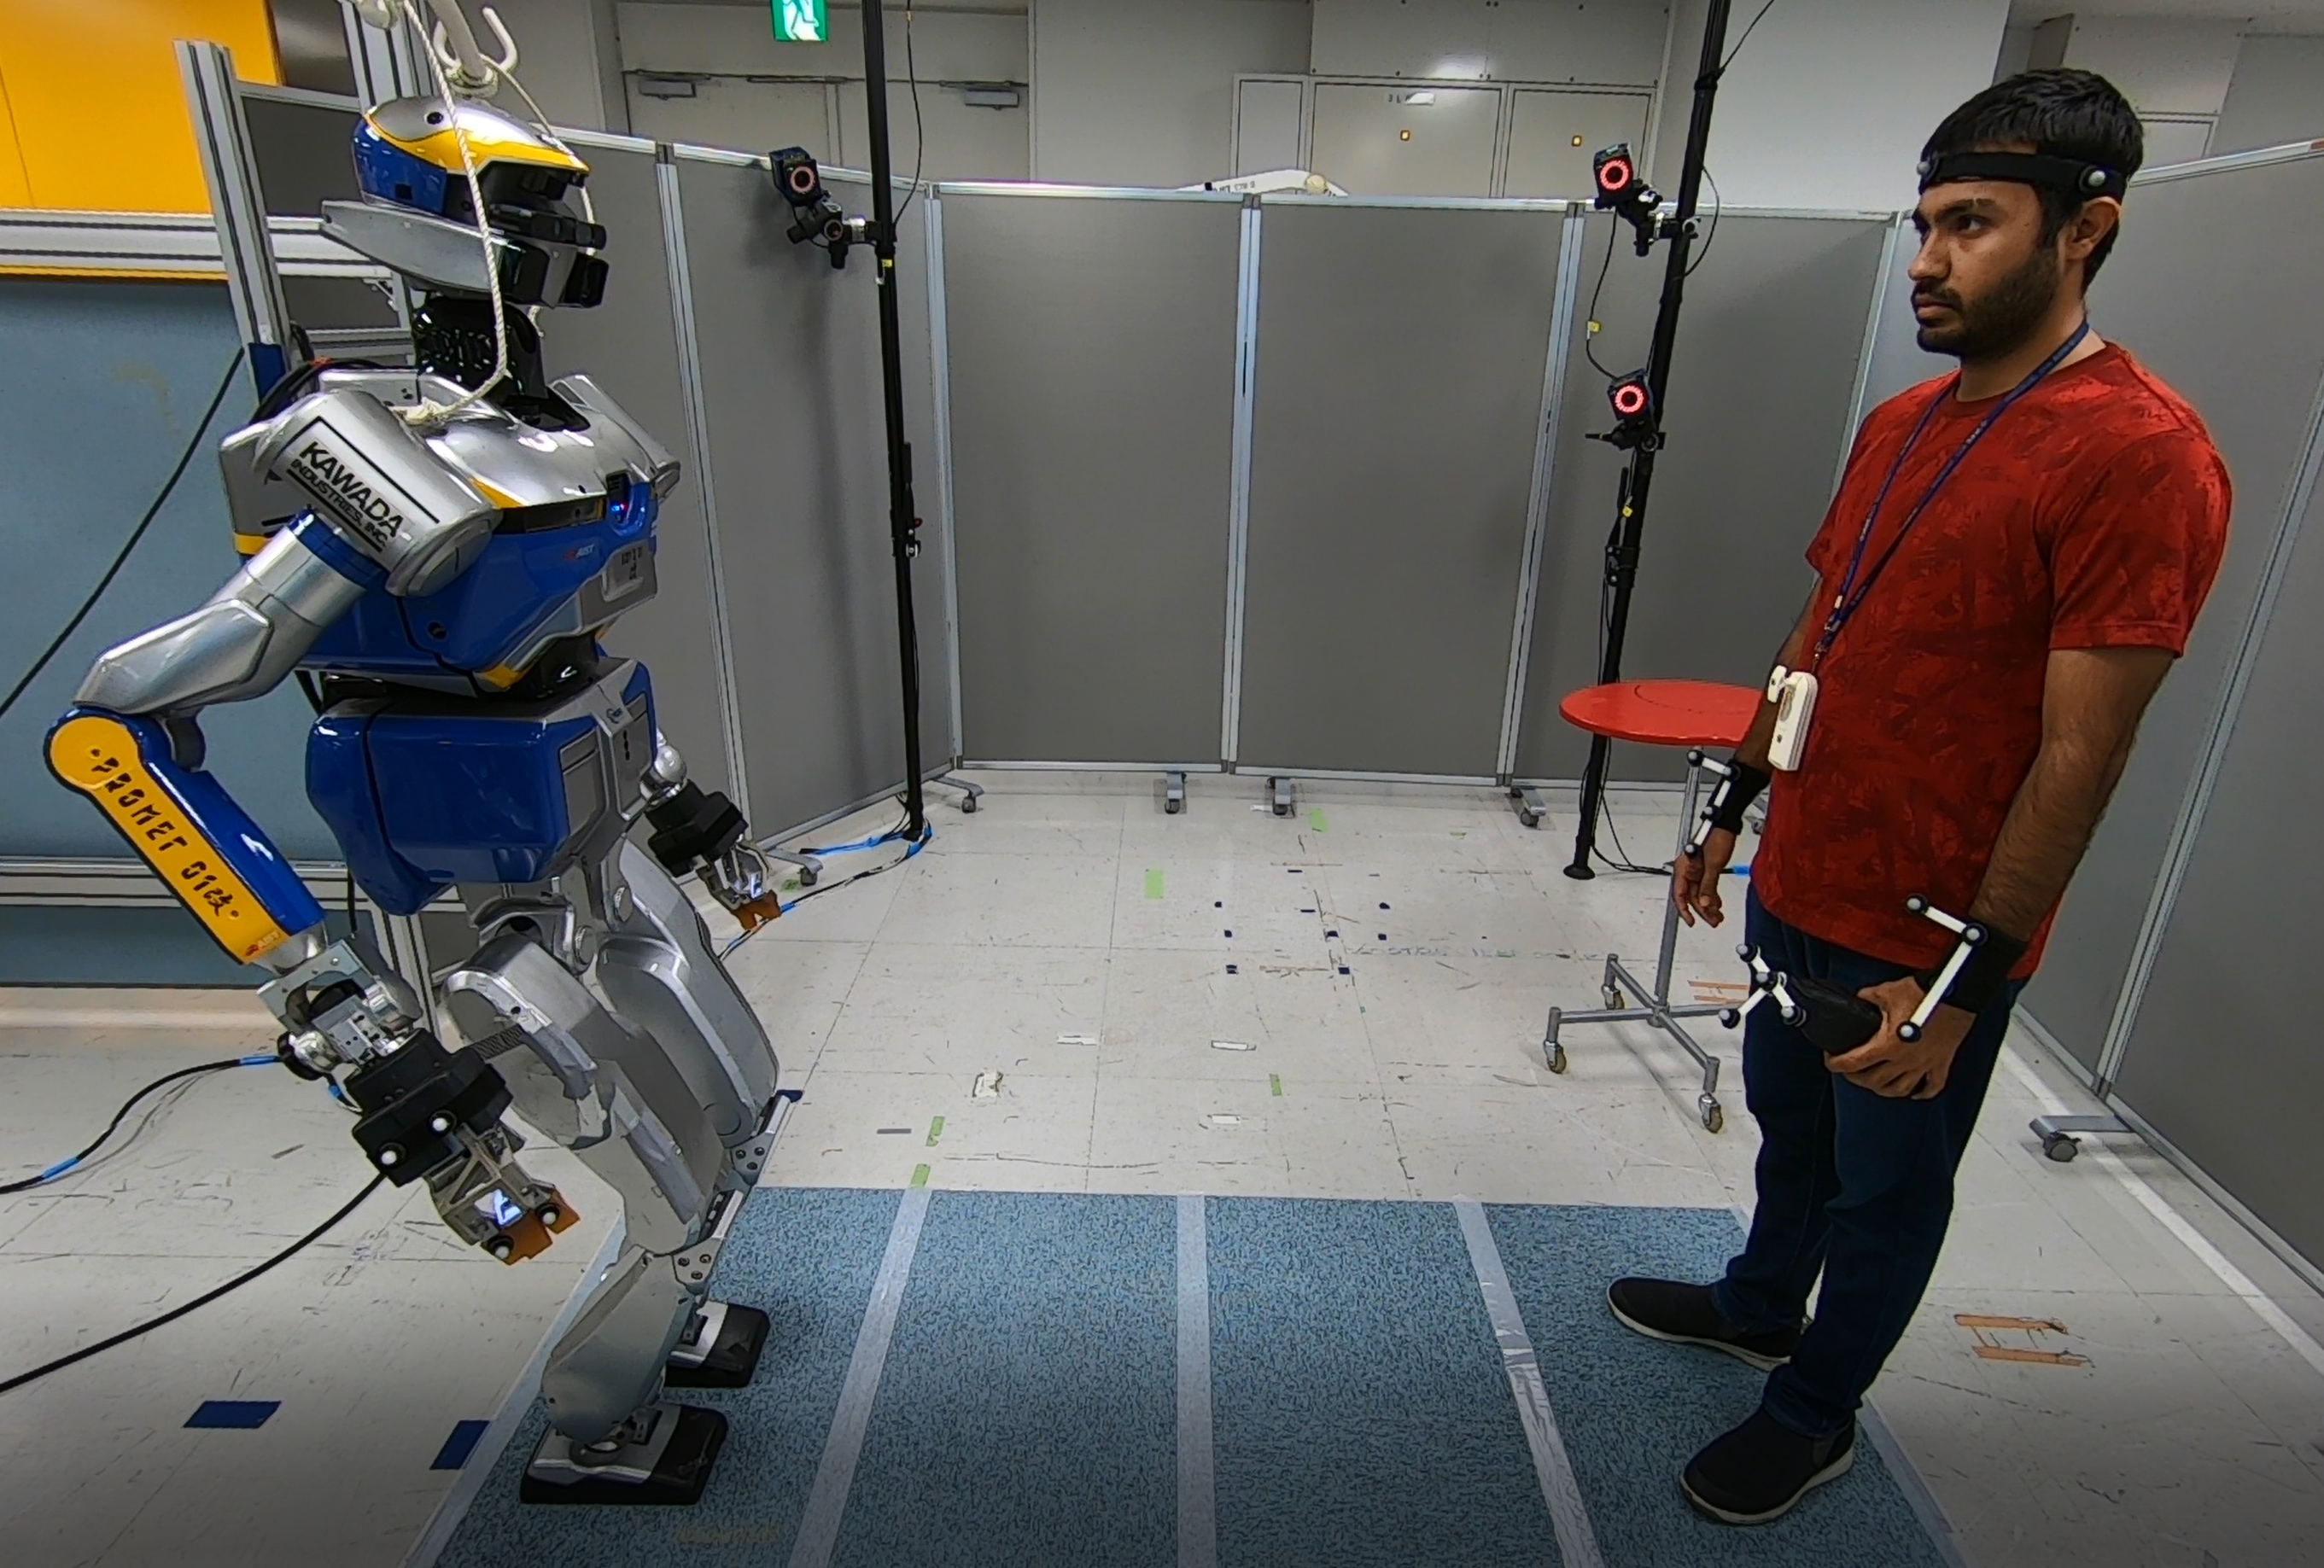
\includegraphics[width=0.8\columnwidth]{plots/c4-plots/halfsit}}
	\caption{Human and humanoid starting posture.}
	\label{fig:halfsit}
\end{figure}


Within the handover routine, both human and robot always start from a standing posture (see Fig.~\ref{fig:halfsit}). The robot standing posture has a Center of Mass CoM(z) height $0.87$ meters. We assume that human is ready with the intention to handover the object if he/she is holding the object in his/her hand. The only predefined condition is that human must seriously exchange the object with a robot in one continuous shot. The human can choose his/her hand configuration, speed, trajectory and the handover location but within the robot's reachable workspace.

During 1$^\text{st}$ \textit{sequence} of handover \textit{routine}, the human carries the object to different handover locations with distinguishable orientations of the object carrying hand and tries to give the object to the robot. Similarly, during 2$^\text{nd}$ \textit{sequence} of handover, human approaches somewhere in the robot reachable workspace to receive the object from robot using his/her choice of hand orientation and preferred handover location. The robot end-effectors reachable workspace is given by equation (\ref{reachable}), object handover can occur as long as estimated handover location is within this region.

\begin{equation}\label{reachable}
\centering
1 = 
\begin{cases}
X_{\min} <= {}^{h}\mathcal{P}_{\text{ef}}(x) <= X_{\max} \quad  \\
Y_{\min} < {}^{h}\mathcal{P}_{\text{ef}}(y) <= Y_{\max} \quad  \\
{}^{h}\mathcal{P}_{\text{ef}}(z) >= CoM(z)

\end{cases}
\end{equation}

where, $ {}^{h}\mathcal{P}_{\text{ef}} $ is the relative 3D position of active human hand \texttt{w.r.t} robot end-effector. The default values of $ X_{\min} $ and $ X_{\max} $ are $ 0.1 $ and $ 0.8 $ meters respectively, for robot left end-effector $ Y_{\min} $ and $ Y_{\max} $ are $ 0.15 $ and $ 0.75 $ meters respectively, while for robot right end-effector $ Y_{\min} $ and $ Y_{\max} $ are $ -0.75 $ and $ 0.15 $ meters respectively.

Just like during human-human object handover, another thing that we incorporated in our handover \textit{routine} is to give visual tracking like behaviour to HRP-2Kai by following an object or active human hand using robot's head, depending on the handover \textit{sequence}. Using a \texttt{gaze} task (\nameref{QPTasks}), HRP-2Kai follows object during 1$^\text{st}$ \textit{sequence} of handover and follows active human hand which is approaching to retrieve the object during 2$^\text{nd}$ \textit{sequence}.

Hereafter and until section (\nameref{both hands individual}) we will formulate the handover \textit{routine} using human right hand and robot left end-effector; afterwards we will generalize our one-handed handover \textit{routine} for four possible handover combination scenarios:

\begin{itemize}
	\item \textbf{human right hand $\longleftrightarrow$ robot left end-effector}
	\item human left hand $\longleftrightarrow$ robot left end-effector 
	\item human left hand $\longleftrightarrow$  robot right end-effector
	\item human right hand $\longleftrightarrow$ robot right end-effector
\end{itemize}


\begin{figure}[pt]
	\centering
	\tikzstyle{line} = [draw, -latex']
	
	\tikzstyle{cloud} = [draw, ellipse,fill=blue!20, text width=6em, text centered, node distance=4cm,  inner sep=0pt, minimum height=2em]
	
	\tikzstyle{startstop} = [rectangle, text centered, rounded corners, minimum width=3cm, minimum height=1cm, draw=black, node distance=4cm, fill=red!30]
	
	\tikzstyle{io} = [trapezium, trapezium left angle=70, trapezium right angle=-70,text centered, text width = 1cm,minimum height=1cm, minimum width=2cm, node distance=4cm, draw=black, fill=red!30]
	
	\tikzstyle{process} = [rectangle, text centered, minimum width=1cm, minimum height=1cm, draw=black, fill=orange!30]
	
	\tikzstyle{block} = [rectangle, draw, fill=green!20, text width=10em, text centered, node distance=4cm, minimum height=4em]
	
	\tikzstyle{decision} = [diamond, draw, fill=yellow!20, text width=6em, text badly centered, node distance=4cm, inner sep=0pt]
	
	\begin{tikzpicture}[node distance = 3cm, auto]
	
	\node [process] (or) {1$^\text{st}$ or 2$^\text{st}$ \textit{sequence}};
	
	\node [startstop, above of=or, node distance = 2cm, auto] (start) {start handover routine};	
	
%	\node [cloud, left of=or] (subj) {human has object};
%	\node [cloud, right of=or] (robot) {robot has object};
	
	\node [block, below of=or, node distance=2cm] (init) {initialize prediction model};
	\node [io, right of=init] (in1) {robot Ef pose};
	\node [io, left of=init] (in2) {human hand pose};
	
	\node [block, below of=init, node distance = 3cm, auto] (relativePos) {observe and track active human hand pose relative to robot Ef pose};
	
	\node [decision, below of=relativePos] (within) {has human hand arrived within robot's reachable workspace?};
	
%	\node [block, left of=within, node distance=5cm, text width=5em] (wait) {wait \& head-track human hand};
	
	\node [decision, right of=within, node distance=5cm, text width=5em] (walk) {did human moved backward?};
	
	\node [block, below of=walk, node distance=3cm, text width=5em] (trigger) {trigger walk};
	
	\node [block, below of=within, node distance=4cm] (moveEf) {start moving robot Ef to predicted position};
	
	\node [decision, below of=moveEf, node distance = 4cm] (ifClose) {is human hand close enough to robot?};
	
	\node [block, right of=ifClose, node distance = 5.5cm] (keep moving) {keep moving Ef towards predicted position};
	
	
	\node [startstop, below of=ifClose, node distance=3cm] (event) {handover object};
	
	% Draw edges
%	\path [line] (subj) -- (or);
%	\path [line] (robot) -- (or);
	\path [line] (start) -- (or);
	\path [line] (or) -- (init);
	
	\path [line,dashed] (in1) -- (init);
	\path [line,dashed] (in2) -- (init);
	\path [line] (init) --  node {FSM} (relativePos);
	\path [line] (relativePos) -- (within);
	
%	\path [line] (wait) |- (relativePos);
%	\path [line] (within) -- node [near start] {no} (wait);
	\path [line] (within) -- node {yes} (moveEf);
	
	\path [line] (within) -- node [near start] {no} (walk);
	\path [line] (walk) -- node [near start] {yes} (trigger);
	\path [line] (walk) |- node [near start] {no} (relativePos);
	
	\path[line] (moveEf) -- (ifClose);
	\path [line] (ifClose) -- node [near start] {no} (keep moving);
	\path [line] (ifClose) -- node [near start] {yes} (event);
	
	\end{tikzpicture}
	
	\caption{General overview of human humanoid handover \textit{sequence}. 1$^\text{st}$ (human has object) or 2$^\text{nd}$ (robot has object).}
	\label{fig:handover routine}
\end{figure}


\section{Experimental setup}

Our experiment setup is shown in (Fig.~\ref{fig:halfsit}). Initially, we started by having a human co-worker and robot co-worker standing comfortably in front of each other at a distance of $1.2$ meters from each other. This distance is known to be the social distance in human proxemics~\cite{hall1966proxemic}. Movable panels partially enclosed the whole setup.

\subsection{Robot}

We used an HRP-2Kai robot~\cite{Kaneko:RAS_ICHR:2015} as the co-worker. The human and humanoid are free to use their both hands, end-effectors respectively in handing over the objects.

\subsection{Mocap}

We used motion capture (in short \textit{mocap}) system manufactured by ({\it Motion Analysis Co.,}), to track and get the position data of the passive reflective markers. We used twenty passive reflective markers in several handover scenarios. We placed four markers on each end-effectors, three markers were placed on the head of the human co-worker to get his/her position in mocap frame, three markers were placed on each of the hands of a human co-worker and also on the object itself. The markers on the human hands and object were utilized to get their respective position, and orientation in the mocap frame and we used makers on the robot end-effectors during object handover and release-return of object from the robot grippers to human co-worker as a substitute to lack of haptic feedback, see section (\nameref{interaction model}) for more details. These passive markers were tracked using ten kestrel infra-red cameras, each at 200 Hz. These mocap markers position data was utilized using a real-time interface between mocap system (\texttt{cortex}) and \texttt{ROS} called \textit{ros-cortex-bridge}, which was designed to transmit this position data to the robot controller in real-time.

\subsection{Handover object(s)}

As shown in (Fig.~\ref{fig:objects}), we used three easily distinguishable objects during the one-handed handover between the human-humanoid dyad. The mass of objects varies from $0.22$ kg to $1.1$ kg.


\begin{figure}[H]
	\centering{\includegraphics[width=0.4\columnwidth]{plots/c4-plots/objects}}
	\caption{Distinguishable shape and mass objects used during one-handed handover between human and humanoid co-worker.}
	\label{fig:objects}
\end{figure}

\section{Robot QP controller}\label{QPController}

We used our research group's native multi-objective Quadratic Programming (QP)~\cite{ladder-HRP-2Kai} based low-level Whole-Body Control (WBC) to govern and optimize the motion of HRP-2Kai. ``WBC exploits the full potential of the entire floating based robot body and allows interaction with the environment using multi-contact strategies''. It also allows concurrent execution of several tasks at once, for example using WBC, the humanoid can utilize one or both of its end-effector(s) to grasp and manipulate the object while at the same time takes a step forward or backward, allowing itself to reach the handover location. 

To realize human, humanoid bi-directional object/tool handover, we introduced several tasks and formulated them in a quadratic fashion, so it conforms with QP based controller. The QP enables whole-body control of our HRP2-Kai while respecting both internal and external constraints. Few such constraints encompass joints limits, force and torque limits, contact constraints, stability constraints such as keeping the centre of mass (CoM) inside the support polygon along with self-collision constraints with the environment and itself while generating optimal joint trajectories. Below we mentioned some significant constraints that a robot must satisfy at each time step during human-robot object handover.


\subsection{QP constraints}\label{QPConstraints}

The QP controller's objective is to compute an acceleration of $\ddot{q}$, where $q$ is the robot configuration vector at each time step ($dt$)  to achieve a set of targets or tasks. At each $dt$, the QP is formulated and solved by the LSSOL solver~\cite{gill1986fortran}. The tasks are formulated either linear constraints or quadratic costs~\cite{ladder-HRP-2Kai}. However, we want to solve these tasks in a best possible manner as a linearization of some tasks may not be feasible or maybe conflicting, therefore using least-square approximation, the quadratic cost $c$ corresponding to a task $\mathscr{T}_i =0$ is given by:


\begin{equation}
c_i(q,\dot{q}, \ddot{q})  = \frac{1}{2}{\norm{ J_i\ddot{q} + \dot{J}_i\dot{q} -\ddot{\mathscr{T}}_i }^2 }
\end{equation}

where $J_i$ the Jacobian matrix of $\mathscr{T}_i$, and the quadratic objective function of QP controller would be,

\begin{equation}\label{qp equation}
\min_{\ddot{q},\tau,f} \; \sum_{i\in O} \omega_i c_i(q,\dot{q},\ddot{q}) + \omega_{f}\lVert f\rVert^2
\end{equation}

which is subject to constraint on equation of motion, as well as other below mentioned constraints,

\begin{equation}
	M(q)\ddot{q} + N(q,\dot{q}) =  J_c^T f
\end{equation}

where $f$ is the set of contact forces, $M$ denotes the inertial matrix of the robot, $N$ accounts for Coriolis and gravity effects, $J_c$ is the Jacobian matrix of all points of contact. 

The QP objective function in equation (\ref{qp equation}) is made of two terms and the tasks $\mathscr{T}_i$ mentioned in next subsection (\nameref{QPTasks}) are weighted against each other by weight $w_i$ based on their relative importance and priority. While the damping weight $w_f$ ensures the smoothness and uniqueness of solution by keeping Hessian matrix positive definite.

\begin{enumerate}	
	\item Static equilibrium:

	$\underline{\tau} \leq J^i(q_i)^Tf_i - g^i(q_i) \leq \overline{\tau}$
	
	where sub-script or super-script $i$ is the $i$-th robot, $q_i$ is the $i$-th robot configuration vector, $f_i$ is the set of contact forces vector of $i$-th robot, $J$ is the Jacobian matrix of all points of contact forces, and $\overline{\tau}$ and $\underline{\tau}$ are the maximum and minimum steady state torque limits respectively, and g be the gravity constant.
	
	\item Joint limits:
	
	$\underline{q_i} \leq q_i \leq \overline{q_i}$
	
	$\underline{q_i}$ and $\overline{q_i}$ are the lower and upper limits for robot joints.
	
	\item Self collisions:
	
	$\delta(X^i_j(q_i), X^i_k(q_i)) > \epsilon_{jk} \qquad \forall(j,k)\in {\mathscr{I}}^i_{\text{self\;collision}}$

	$\delta$ is the function of distance, $X^i_j(q_i)$ is the occupied volume by $j$-th body of robot in configuration $q_i$, $\epsilon_{jk}$ is the pair of user select minimum distances ($j$,$k$) and ${\mathscr{I}}^i_{\text{self\;collision}}$ is the robot sets of self collision pairs.
	
	\item Environment collision:
	
	$\delta(X^i_j(q_i), X_k) > \epsilon_{jk} \qquad \forall(j,k)\in {\mathscr{I}}^i_{\text{robot\;environment}}$
	
	${\mathscr{I}}^i_{\text{robot\;environment}}$ is the set of robot environment (object) collision pairs.
	
	\item Contact Constraint: $\mathscr{I}_\text{contact} = J_i(q) (\dot{q}_{s(k)} - \dot{q}_{p(k)}) = 0$\\
	The objective of this constraint is to maintain a null velocity~\cite{ohwovoriole1980externsion} between the joints of bodies in contact, where $p(k)$ and $s(k)$ are the predecessor and successor bodies of a robot(s) in contact that imposes a constraint~\cite{featherstone2014rigid}.
\end{enumerate}

%%%	\item acceleration Constraint: $\mathscr{I}_{contact} = J_i(q)\ddot{q}_{s(k)} + \dot{J}(q)_i\dot{q}_{p(k)} = 0$\\


\subsection{QP tasks}\label{QPTasks}

As mentioned earlier, below, we introduced the following outlined tasks to the multi-objective QP controller to achieve safe and reliable human-robot object handover. Let function $\mathscr{T}_i(q)$ denote the geometric objectives (task error) that we require to regulate to zero or maintain above zero, i.e. $\mathscr{T}_i(q) = 0$ and $\mathscr{T}_i(q) \geq 0$.  

\begin{enumerate}[start=1,label={\arabic*.}]

\item Posture task: $\mathscr{T}_\text{posture} = q_d - q = 0$\\
Posture task is the first task that is added to the QP controller, it allows the robot to maintain an initial posture.

\item Com task: $\mathscr{T}_\text{CoM} = \text{CoM}_d - \text{CoM}(q) = 0$\\
Com task is used in conjunction with the stability constraint to all time maintain the CoM position inside the support polygon. 

\item Joint limit task: $\mathscr{T}_\text{jlim} = \underline{q_i} \leq q_i \leq \overline{q_i}$\\
This task is used occasionally whenever there is a need to limit certain joint movements.  

\item Position task at body $k$: $\mathscr{T}_\text{pos} = r^d_k - r_k(q) = 0$\\
Where, $r_k$ and $r^d_k$ are the current and desired position of $i$-th robot $k$-th body. Robot end-effector position task is used to reach the desired handover location~\cite{ladder-HRP-2Kai}.

\item Orientation task at body $k$: $\mathscr{T}_\text{ori} = Err((E^d_k),  E_k(q))$\\
Where, $E_k$ is the orientation of $i$-th robot body to world. Robot end-effector orientation task is used to compute orientation relative to human hand orientation.

\item Gaze task : $\mathscr{T}_\text{gaze} =u_\text{target} - u = 0$\\
Where, $u_\text{target}$  and $u$ are the target vector in world and body vector that needs to be oriented respectively. We used gaze task to orient the head joints of HRP-2Kai towards the active human hand position in the world; more details can be found in~\cite{samy2017VecOriTask}. Note that by active human hand we meant by either object carrying human hand during human-to-robot handover trial or by the hand which is approaching to grasp the object during robot-to-human handover trial.

\end{enumerate}


%\clearpage

\section{Notations}

Let $\mathcal{M}$ (Mocap) and $\mathcal{R}$ (Robot) be the two fixed frames with the same orientation that represent both Cartesian coordinate systems and Pl\"ucker coordinate systems denoted by $X$ in the Euclidean space. Both $\mathcal{M}$ and $\mathcal{R}$ are defined by their position and orientation of a Cartesian frame, such that ${}^MX_R$ denotes the Pl\"ucker coordinate transform which depends only on the position and orientation of frame $\mathcal{M}$ relative to frame $\mathcal{R}$ (see Fig~\ref{fig:frames}).

\begin{figure}[ht]
	\centering{\includegraphics[width=0.5\columnwidth]{plots/c4-plots/frame}}
	\caption{$\mathcal{M}$ and $\mathcal{R}$ Cartesian coordinate systems.}
	\label{fig:frames}
\end{figure}


\begin{itemize}	
	\item  We used 6D spatial vectors to express the pose of human hands and robot end-effectors as well as objects. We, therefore, adopt a 6D notation based on spatial vectors, which was explained in Chapter 2 of~\cite{featherstone2014rigid}.
		
	\item One can receive and control the robot end-effector current orientation ${{}^{\text{ef}}\mathcal{O}_R} \in \mathbb{R}^{3\times3}$ and current position ${{}^{\text{ef}}\mathcal{P}_R} \in \mathbb{R}^{3}$ respectively in the $\mathcal{R}$ frame, by using QP's \texttt{Orientation} task and \texttt{Position} task (see subsection~\nameref{QPTasks}), therefore,
	\begin{gather}\label{X_R_ef}
	{}^{\text{ef}}{X}_R =
	\left[\begin{array}{cc}
	{}^{\text{ef}}\mathcal{O}_R & {}^{\text{ef}}\mathcal{P}_R
	\end{array}\right]
	\end{gather}
	
	\item Likewise, ${{}^{h}\mathcal{O}_M} \in \mathbb{R}^{3\times3}$ and ${{}^{h}\mathcal{P}_M} \in \mathbb{R}^{3}$, denotes the human hand $h$ orientation and position respectively in the $\mathcal{M}$ frame, obtained from the ${\bf L}$ shape body (see Fig.~\ref{fig:lshapes}), which is later further explained in section (\nameref{orientation_model}),
	\begin{gather}\label{X_M_h}
	{}^{h}{X}_M =
	\left[\begin{array}{cc}
	{}^{h}\mathcal{O}_M & {}^{h}\mathcal{P}_M \\
	\end{array}\right]
	\end{gather}
	
	\item ${{}^{h}\mathcal{O}_{\text{ef}}} \in \mathbb{R}^{3\times3}$ and ${{}^{h}\mathcal{P}_{\text{ef}}} \in \mathbb{R}^{3}$ respectively, denotes the human hand $h$ orientation and position relative to robot end-effector,
	\begin{gather}\label{X_ef_h}
	{}^{h}{X}_{\text{ef}} =
	\left[\begin{array}{cc}
	{}^{h}\mathcal{O}_{\text{ef}} & {}^{h}\mathcal{P}_{\text{ef}} \\
	\end{array}\right]
	\end{gather}
	
	\item Let ${{}^{o}\mathcal{O}_M} \in \mathbb{R}^{3\times3}$ and ${{}^{o}\mathcal{P}_M} \in \mathbb{R}^{3}$, denotes the object orientation and position respectively in the $\mathcal{M}$ frame, obtained from another ${\bf L}$ shape body (see Fig.~\ref{fig:lshapes}) attached on the object.
	\begin{gather}\label{X_M_o}
	{}^{o}{X}_M =
	\left[\begin{array}{cc}
	{}^{o}\mathcal{O}_M & {}^{o}\mathcal{P}_M \\
	\end{array}\right]
	\end{gather}
	
	\item For convenience, we formulated the problem with a common origin {\it O}, such that $\mathcal R \equiv M$ (both frames are located between the feet of robot HRP-2Kai), therefore, we can get human hand pose \texttt{w.r.t.} or relative to robot end-effector
	\begin{equation}\label{X_ef_h1}
	{}^{h}{X}_{\text{ef}} = {}^{h}{X}_{M}  {}^{\text{ef}}{X_{R}}^{-1}
	\end{equation}
	\item otherwise, when $\mathcal R \neq M$, using Pl\"ucker transform ${}^MX_R$,
	
	\begin{equation}\label{X_ef_h2}
	{}^{h}{X}_{\text{ef}} = {}^{h}{X}_{M}  {\bf{}^{M}{X}_R}  {}^{\text{ef}}{X_{R}}^{-1}
	\end{equation}

\end{itemize}


\begin{figure}[htpb]
	\centering{\includegraphics[width=.9\columnwidth]{plots/c4-plots/lshpe-lt-rt}}
	\caption{${\bf L}$ shape rigid body on the human hand(s)}
	\label{fig:lshapes}
\end{figure}

Note that, the mathematical notations in the following sections follow ISO guidelines. The Euclidean distance is represented in meters. The time unit is set in seconds or mentioned otherwise.


\section{Position prediction model}\label{prediction_model}

In case of object handover and when the human co-worker is ready with the intention to handover the object, instead of merely waiting for the object to be presented by the human at the handover location, the robot must proactively plan its own movements by observing past and predicting near-future human hand movements so that it could arrive at the human chosen handover location approximately at same time ---either to receive or return the object. Therefore, the estimation of handover time, as well as the approximation of handover location, must be realized early during the handover \textit{sequence}. Note that this proactive nature of the robot co-worker should also be available when the human co-worker requests for the object.

Here we designed a prediction model, with robot left end-effector pose $\mathcal{}^{\text{ef}}{X}_R$ (\ref{X_R_ef}) and human hand mocap marker position ${}^{h}\mathcal{P}_M$ (\ref{X_M_h}) as inputs. Note that for simplicity, we formulated the problem with a common origin {\it O}, such that frame $\mathcal R \equiv M$. To get the position and orientation of the human hand, we placed a rigid body with a shape similar to an alphabet ${\bf L}$ on the wrist of a human hand(s) and on the object as shown in (Fig.~\ref{fig:lshapes}). The three mocap markers $A, B$ and $C$ make up the three vertices of ${\bf L}$ shape body. Note that from onward by ${}^{h}\mathcal{P}_M$ we would mean the position of point $A$ on the ${\bf L}$ shape body as the human hand marker position (Fig.~\ref{fig:lshapes}).

The prediction model behaviour can be tuned by two initially required constant sample size, $i_\text{observe}$ ---a predefined sample size required to observe the motion of the human hand and $i_\text{predict}$ ---required to predict the human hand position in advance.

In order for the handover between human and humanoid to be smooth and intuitive, the robot needs to proactively estimate the near future position of human hand in advance, during both \textit{sequence}s when robot act as receiver (1$^\text{st}$ \textit{sequence}) or when robot acts as giver (2$^\text{nd}$ \textit{sequence}) of a handover \textit{routine}. Therefore we formulate the movements of the human hand as a constant velocity based linear motion model to predict his/her hand (hence handover) position continuously. The robot observes human hand movements for a predefined sample size $i_\text{observe}$ along with the average velocity of his/her hand during that time and then predicts the near future human hand movement direction and position using equations (\ref{predictVel}) and (\ref{predict}) for the predefined  $i_\text{predict}$ sample size.

\begin{equation} \label{predictVel}
{}^{h}\mathcal{\bar{V}}_{M} = \frac{1}{i_\text{observe}}{\sum_{j=1}^{j=i_\text{observe}} ({}^{h}\mathcal{P}_{M}(j)-{}^{h}\mathcal{P}_{M}(j-1))/dt }
\end{equation}

\begin{equation} \label{predict}
{}^{h}\mathcal{P}_M(i_\text{predict}) = {}^{h}\mathcal{\bar{V}}_{M} \cdot (i_\text{predict}  - i_\text{observe})  \cdot dt + {}^{h}\mathcal{P}_{M}(i_\text{observe})
\end{equation}


where $dt$ is controller run-time, in our case it is 5ms as mentioned earlier in the section (\nameref{QPController}). $j$ in equation (\ref{predictVel}) is sample index. ${}^{h}\mathcal{\bar{V}}_{M}$ is the average human hand movement velocity during $i_\text{observe}$ sample size. ${}^{h}\mathcal{P}_M(i_\text{predict})$ is the predicted position of human hand at $i_\text{predict}$. The prediction model updates and converges itself over time and in doing so updates the robot end-effector position towards the active human hand, upon condition if predicted position is within the robot end-effector's reachable workspace. 

Recalling equation (\ref{X_ef_h1}) or (\ref{X_ef_h2}), the updated translation component of pl\"ucker transformation ${}^{h}{X}_{\text{ef}}$, which provides the predicted position of human hand with respect to robot end-effector in the robot coordinate system is given by (\ref{X_ef_ht}).

\begin{equation}\label{X_ef_ht}
{}^{h}{X}_{\text{ef}}(i_\text{predict}) =  {}^{h}{X}_M  {}^{M}{X}_R {{}^{\text{ef}}{X}_R}^{-1}
\end{equation}

where, ${}^{M}{X}_R$ is the Pl\"ucker coordinate transform frame $\mathcal{M}$ relative to frame $\mathcal{R}$, if $\mathcal R \neq M$.


Finally, the handover location is estimated based on the human hand predicted position when the following conditions satisfy (\ref{min_posErr_vel}), that is when the human hand velocity is minimum and robot end-effector is closest to the human hand.

\begin{equation}\label{min_posErr_vel}
\begin{cases}
	\norm{{}^{h}\mathcal{\bar{V}}_{M}}& <= 1e^{-2} \\
	\norm{({}^{h}\mathcal{P}_{M}(i_\text{predict}) - {}^{\text{ef}}\mathcal{P}_{R})} & <= 2e^{-2}
\end{cases}
\end{equation}

where, ${}^{h}\mathcal{P}_{M}(i_\text{predict})$ is the desired position for robot end-effector to reach and ${}^{\text{ef}}\mathcal{P}_{R}$ is the actual current position of robot end-effector and also both positions are in same frame or transformed otherwise. We have also explained the procedure of predicting human hand position and estimating handover location in Algorithm (\ref{positionalgo}) of (\nameref{handoverAppendix}).

In this section, we presented how to predict and estimate the handover location, though just by knowing the handover location in space is not enough for an optimal smooth handover of an object. Therefore in next section (\nameref{orientation_model}), we will present the orientation component of ${}^{h}{X}_{\text{ef}}$ which gives the graspable relative orientation of robot end-effector \texttt{w.r.t} human hand or object orientation during handover.


\section{Grasp configuration model}\label{orientation_model}

To take into account comfort and requirement of the human co-worker, it is pivotal for the robot to be able to find the most appropriate configuration to grasp (as \textit{receiver}) or release (as \textit{giver}) the object~\cite{cakmak2011human, aleotti2012comfortable}. Therefore for an intuitive and smooth handover of an object, the robot should relatively orient it's end-effector and configure according to the orientation of either object (1$^\text{st}$ \textit{sequence}) or human hand (2$^\text{nd}$ \textit{sequence}) during the handover \textit{routine}. Though there are several possible configurations to handover an object, the robot must determine the correct configuration of its end-effector during the handover which is suitable and comfortable enough for the human and could be perceived natural in the eyes of a human co-worker. Note that in this study, we mainly chose to handover the object in which it is most commonly being grasped (default configuration) hence natural to the eyes of the human, one example would be holding an object such as a water bottle when its cap is in the upright position during the handover. 

We propose a simple method to get the desired object grasping orientation of robot end-effector either by considering the relative orientation of the active human hand or the object itself. This handover grasp configuration model consists of two sub-models, in first sub-model, we determine the orientation of the active human hand or object itself. In the second sub-model, we utilize the first sub-model to continuously get the desired relative orientation of the robot end-effector during the handover \textit{routine}. 


%%% 1st sub-model

To determine the object or active human hand orientation, as  mentioned in previous section we placed an ${\bf L}$ shape rigid body on the wrist of the human hand(s) and a similar one on the object as well such that during the object handover scenario, vector $\vec{AB}^{\,}$ along the longer side and vector $\vec{BC}^{\,}$ along the shorter side of the ${\bf L}$ shape are set to be parallel with the $X$-axis and $Y$-axis of the mocap frame $\mathcal{M}$ respectively, as well as orthogonal to each other (as shown in Fig.~\ref{fig:lshapes}). For simplicity, let us consider $\hat{x}$ be the unit vector, which is parallel and along the $X$-axis and likewise a unit vector $\hat{y}$ is parallel and along the $Y$-axis of the mocap frame $\mathcal{M}$, such that

\begin{equation*}
\hat{x} = \frac{\vec{AB}^{\,}}{\norm{\vec{AB}^{\,}}}
\end{equation*}

\begin{equation*}
\hat{y} = \frac{\vec{BC}^{\,}}{\norm{\vec{BC}^{\,}}}
\end{equation*}

Let ${}^{h}\mathcal{O}_{M}$ in equation (\ref{X_M_h}) be the rotation matrix representing the orientation of human hand (or object) in the mocap frame $\mathcal{M}$ and since $\hat{x} \in \mathbb{R}^{3}$ and $\hat{y} \in \mathbb{R}^{3}$ are the two orthogonal unit vectors of an ${\bf L}$ shape body on each human hand (Fig.~\ref{fig:lshapes}), therefore a cross product of them would result in another unit vector $\hat{z} \in \mathbb{R}^{3}$ which is also orthogonal to both $\hat{x}$ and $\hat{y}$. Also using right-hand rule, one can easily get the direction of the unit vector $\hat{z}$ by given equation (\ref{cross}).

\begin{equation}\label{cross}
\hat{z} = \hat{x} \times \hat{y}
\end{equation}

Furthermore, to represent the orientation of human hand in $\mathbb{R}^{3\times3}$, we used these unit vectors $\hat{x}, \hat{y}$ and $\hat{z}$ as columns of the rotation matrix ${}^{h}\mathcal{O}_{M}$~\cite{evans2001rotations, altmann2005rotations, jia2017rotation} in equation (\ref{rotationmatrix}), such that these unit vectors $\hat{x}, \hat{y}$ and $\hat{z}$ represent human hand (or object) orientation around the $roll-pitch-yaw$ axes, respectively.

\begin{equation}\label{rotationmatrix}
{}^{h}\mathcal{O}_{M} = 
\left\{\begin{array}{cccc}
\hat{x.x} & \hat{y.x} & \hat{z.x} \\
\hat{x.y} & \hat{y.y} & \hat{z.y} \\
\hat{x.z} & \hat{y.z} & \hat{z.z}
\end{array}\right\}_{3\times 3}
\end{equation}

Therefore, the pose (\ref{X_M_h}) of active human hand or object can be determined using equations (\ref{predict}, translation) and (\ref{rotationmatrix}, orientation). Recalling again that active human hand is the one that carries the object during 1$^\text{st}$ \textit{sequence} or the hand which is approaching to grasp the object during 2$^\text{nd}$ \textit{sequence} of a handover \textit{routine}.

\begin{figure}[htpb]
	\centering{\includegraphics[width=.7\linewidth]{plots/c4-plots/rviz_robot_lt_hand_obj-2layer-empty}}
	\caption{Some possible fixed orientation of HRP-2Kai (left end-effector) during the handover trials in the robot frame $\mathcal{R}$}
	\label{fig:robot_lt_hand_2layers}
\end{figure} 


\begin{figure}[htpb]
	\centering{\includegraphics[width=.7\linewidth]{plots/c4-plots/rviz_robot_lt_hand_obj_frame}}
%	\centering{\includegraphics[width=.7\linewidth]{plots/c4-plots/relaxPos}}
	\caption{HRP-2Kai (left end-effector) holding object with fixed orientation during handover in the robot frame $\mathcal{R}$}
	\label{fig:robot_lt_hand_obj}
\end{figure} 

%%% 2nd sub-model

HRP-2Kai lacks conventional anthropomorphic hands, but instead it has gripper (Fig.~\ref{fig:robot_lt_hand_2layers}) alike hands~\cite{kaneko2015humanoid, stasse2019overview} mainly to increase the manipulability. In this second sub-model, to continuously determine the desired grasping configuration of robot end-effector during the handover, we were first required to know the fixed initial orientation (default) of the robot end-effector and active human hand, in which object handover is feasible between human and robot co-workers. 

Consequently we considered a initial possible scenario where the robot end-effector and active human hand orientations are fixed throughout the handover \textit{routine}, irrespective of the handover \textit{sequence} where robot is a giver or receiver. Let ${{}^\text{efInit}\mathcal{O}_R}$ denote the initial and fixed orientation of the robot end-effector in the robot frame $\mathcal{R}$ as shown in (Fig.~\ref{fig:robot_lt_hand_2layers}, and Fig.~\ref{fig:robot_lt_hand_obj}). Whereas, let ${{}^\text{hInit}\mathcal{O}_M}$ be the fixed grasping configuration of human hand determine by the equation (\ref{rotationmatrix}), such that both,

\begin{equation}\label{fixedOri}
\begin{cases}
{{}^\text{efInit}\mathcal{O}_R}$ $\subset$ ${{}^{\text{ef}}\mathcal{O}_R} \\
{{}^\text{hInit}\mathcal{O}_R}$ $\subset$ ${{}^{h}\mathcal{O}_M}
\end{cases}
\end{equation}

%${{}^\text{efInit}{O}_R}$ $\subset$ ${{}^{\text{ef}}{O}_R}$

Note that both of these fixed subsets in equation (\ref{fixedOri}) of handover grasping configuration for human and robot co-workers are selected before the handover \textit{routine} based on the known physical, structural properties of the object. Since by knowing the object shape, it is possible to determine how a human co-worker would initially grasp the object in its default configuration, assuming that particular grasp is what seemed natural and comfortable to the human co-worker. Also as the active human hand (which grasps the object) has ${\bf L}$ shape body on the wrist, therefore prior to initiating the handover \textit{routine} when human co-worker grasps the object, one can find the ${{}^\text{efInit}\mathcal{O}_R}$ by aligning the vector $\vec{AB}^{\,}$ and $\vec{BC}^{\,}$ of active human hand ${\bf L}$ shape with the global $X$-axis and $Y$-axis respectively.

Now, during the handover \textit{routine} to correctly transform desired human hand orientation into robot end-effector frame, we further utilize the equation (\ref{X_ef_ht}). Using QP's \texttt{Orientation} task~\cite{murray2017mathematical, ladder-HRP-2Kai} (see subsection~\nameref{QPTasks}) and compute the task error $Err$ between \textit{current} human hand orientation ${{}^{h}\mathcal{O}_M}$ obtained using equation (\ref{rotationmatrix}) and \textit{fixed} robot end-effector orientation ${{}^\text{efInit}\mathcal{O}_R}$, the resulting orientation from the \texttt{Orientation} task is the desired robot end-effector orientation relative to the human hand orientation (see Fig.~\ref{fig:robot_lt_orientations}, for few of many possible orientations).

Therefore using fixed orientation component  ${{}^\text{efInit}\mathcal{O}_R}$ and current human hand orientation ${}^{h}\mathcal{O}_M$ from equation (\ref{rotationmatrix}) derived in first sub-model, we further modify equation (\ref{X_ef_ht}) to get the desired orientation $ {}^{h}\mathcal{O}_{\text{ef}} $ of robot end-effector during the handover \textit{routine}.

\begin{gather}\label{X_efinit_hori}
\left[\begin{array}{cc}
\bf{{}^{h}\mathcal{O}_{\text{ef}}} & {}^{h}\mathcal{P}_{\text{ef}}
\end{array}\right] =
\left[\begin{array}{cc}
\bf{{}^{h}\mathcal{O}_M} & {}^{h}\mathcal{P}_M
\end{array}\right]
\left[\begin{array}{cc}
{}^{M}\mathcal{O}_R & {}^{M}\mathcal{P}_R
\end{array}\right]
\left[\begin{array}{cc}
\bf{{}^\text{efInit}\mathcal{O}_{R}} & {}^{\text{ef}}\mathcal{P}_{R}
\end{array}\right]^{-1}
\end{gather}

\begin{figure}[ht]
	\centering{\includegraphics[width=1\columnwidth]{plots/c4-plots/robot_lt_orientations}}
	\caption{Robot HRP-2Kai (left end-effector) multiple possible object grasping configurations during the handover trials in the robot frame $\mathcal{R}$.}
	\label{fig:robot_lt_orientations}
\end{figure} 

Finally, one can get the pose of the handover location by using the translation component of ${}^{h}{X}_{\text{ef}} $ in the equation (\ref{X_ef_h}) which is updated based on the predicted position of active human hand (see section~\nameref{prediction_model}) while the orientation component is updated based on the relative orientation of object during 1$^\text{st}$ \textit{sequence} and active human hand during 2$^\text{nd}$ \textit{sequence} of a handover \textit{routine}.

%\clearpage

\section{Interaction forces model}\label{interaction model}

Another problem that we focused here is related to the \textit{timing} of grasping and releasing the object and minimizing the forces during such interactions. The \textit{timing} at which the robot should close its gripper(s) to grasp the object, if robot tries to close too early to grasp the object when a human co-worker is not ready it can lead to a collision resulting in an accident or if robot waits too long then it may lead to unreliable behaviour. Along with the previously mentioned problem we also address here another issue related with the \textit{magnitude} of interaction forces between human co-worker hand(s) and robot co-worker end-effector(s) holding the object during the release of object in the 2$^\text{nd}$ \textit{sequence} of handover i.e. when robot returns the object to the human.


We had to find the equilibrium for the robot to know the appropriate \textit{timing} at which the handover should occur, which would be intuitive and can be perceived natural to the eyes of human (keeping in mind that HRP-2Kai does not have anthropomorphic hands but rather manipulative grippers). At the same time, we needed to come up with a solution to keep the \textit{magnitude} of interaction forces at a minimum. We came up with two methods to tackle this problem, one highlights the simplicity and other highlights efficiency, but when used together, we get a reliable and safest solution possible under such a scenario.


HRP-2Kai is equipped with 6-axis \textit{wrist} force sensor on both hands, capable of precisely sensing interaction forces and torques with the environment along $x, y, z$ axes of the sensor local coordinate frame (let us call it $s$). We designed a model of interaction forces which enable the robot end-effector to interact with the object independent of the knowledge of the object's mass in advance.


\subsection{Method 1: mocap markers}

Without actual haptic sensor feedback information from the robot end-effector, we had to rely on the wrist force sensor and mocap markers data of the robot end-effector (see Fig.~\ref{fig:markerEf}), therefore we used mocap makers in conjunction with the force feedback from the wrist sensor of HRP-2Kai to know whether the object is within its vicinity to grasp or not. Mocap makers on the robot end-effector were crucial to know the relative position of the object from the active human hand holding it and the robot end-effector. We placed four passive infra-red markers on the robot end-effector(s) in rectangular-shaped configuration as shown in (Fig.~\ref{fig:markerEf}, \ref{fig:markerEf2} and \ref{fig:markerEf1}). Two of the markers were placed parallel and along the local $x$-axis of force sensor on the wrist of robot end-effector and rest two markers were placed on the gripper tips as shown in (Fig.~\ref{fig:markerEf}).

\begin{figure}[ht]
	\centering{\includegraphics[width=.5\linewidth]{plots/c4-plots/markerEf.jpg}}
	\caption{Passive IR markers on the robot HRP-2Kai right end-effector.}
	\label{fig:markerEf}
\end{figure} 


Let \{${}^\text{wa}\vec P, {}^\text{wb}\vec P, {}^\text{ga}\vec P, {}^\text{gb}\vec P$\} $\in \mathbb{R}^{3}$ be the four position vectors of the mocap markers that are placed on the robot end-effector wrist and gripper tips respectively, also let ${}^\text{obj}\vec P\in \mathbb{R}^{3}$ be the position vector of mocap marker that placed on the object as shown in the (Fig.~\ref{fig:robot_lt_hand_obj} and Fig.~\ref{fig:robot_lt_orientations}). To get the relative position of object and active human hand with respect to robot end-effector, assuming human has the object and is ready with the intent to handover the object. We utilized basic linear algebra and vector products~\cite{brand1947vector, crowe1994history, artin2016geometric} to get the area of triangles $\triangle{{}^\text{wa}P {}^\text{wb}P {}^\text{ga}P}$, $\triangle{{}^\text{wa}P {}^\text{wb}P {}^\text{gb}P}$ and $\triangle{{}^\text{wa}P {}^\text{wb}P {}^\text{obj}P}$ using equation (\ref{area general}) such that upon the satisfaction of following conditions in equation (\ref{area bool}) would give us the relative position of object. Basically we were interested in the output of function $f({}^\text{obj}\vec{P})$, this function measures the area of triangles formed by the markers on robot end-effector and the object marker. The positive output means that object is within the graspable reach of robot end-effector and that the robot now is ready to close the gripper.


\begin{equation}\label{area general}
        \triangle{ABC} = \frac{\norm{ \vec{AB} \times \vec{AC} }} {2} \\
\end{equation}
where $\vec{A}$, $\vec{B}$, $\vec{C}$ are the three coordinate vectors of a triangle $\triangle{ABC}$,


\begin{equation}\label{area}
    \centering
    f({}^\text{obj}\vec{P}) = 
    \begin{cases}
     (\triangle{{}^\text{wa}P {}^\text{wb}P {}^\text{ga}P} - \triangle{{}^\text{wa}P {}^\text{wb}P {}^\text{obj}P}) > 0 \\
     (\triangle{{}^\text{wa}P {}^\text{wb}P {}^\text{gb}P} - \triangle{{}^\text{wa}P {}^\text{wb}P {}^\text{obj}P}) > 0
   \end{cases}         
\end{equation}

\begin{equation}\label{area bool}
    \centering
    if
    \begin{cases}
     f({}^\text{obj}\vec{P})==1, & \text{within graspable reach}  \\
     f({}^\text{obj}\vec{P})==0, & \text{object outside gripper}
   \end{cases}         
\end{equation}



\begin{figure}[ht]
	\centering{\includegraphics[width=.8\linewidth]{plots/c4-plots/efmarkers}}
	\caption{Passive IR markers on the robot HRP-2Kai right end-effector, human right hand and object during handover.}
	\label{fig:markerEf2}
\end{figure} 

\begin{figure}[ht]
	\centering{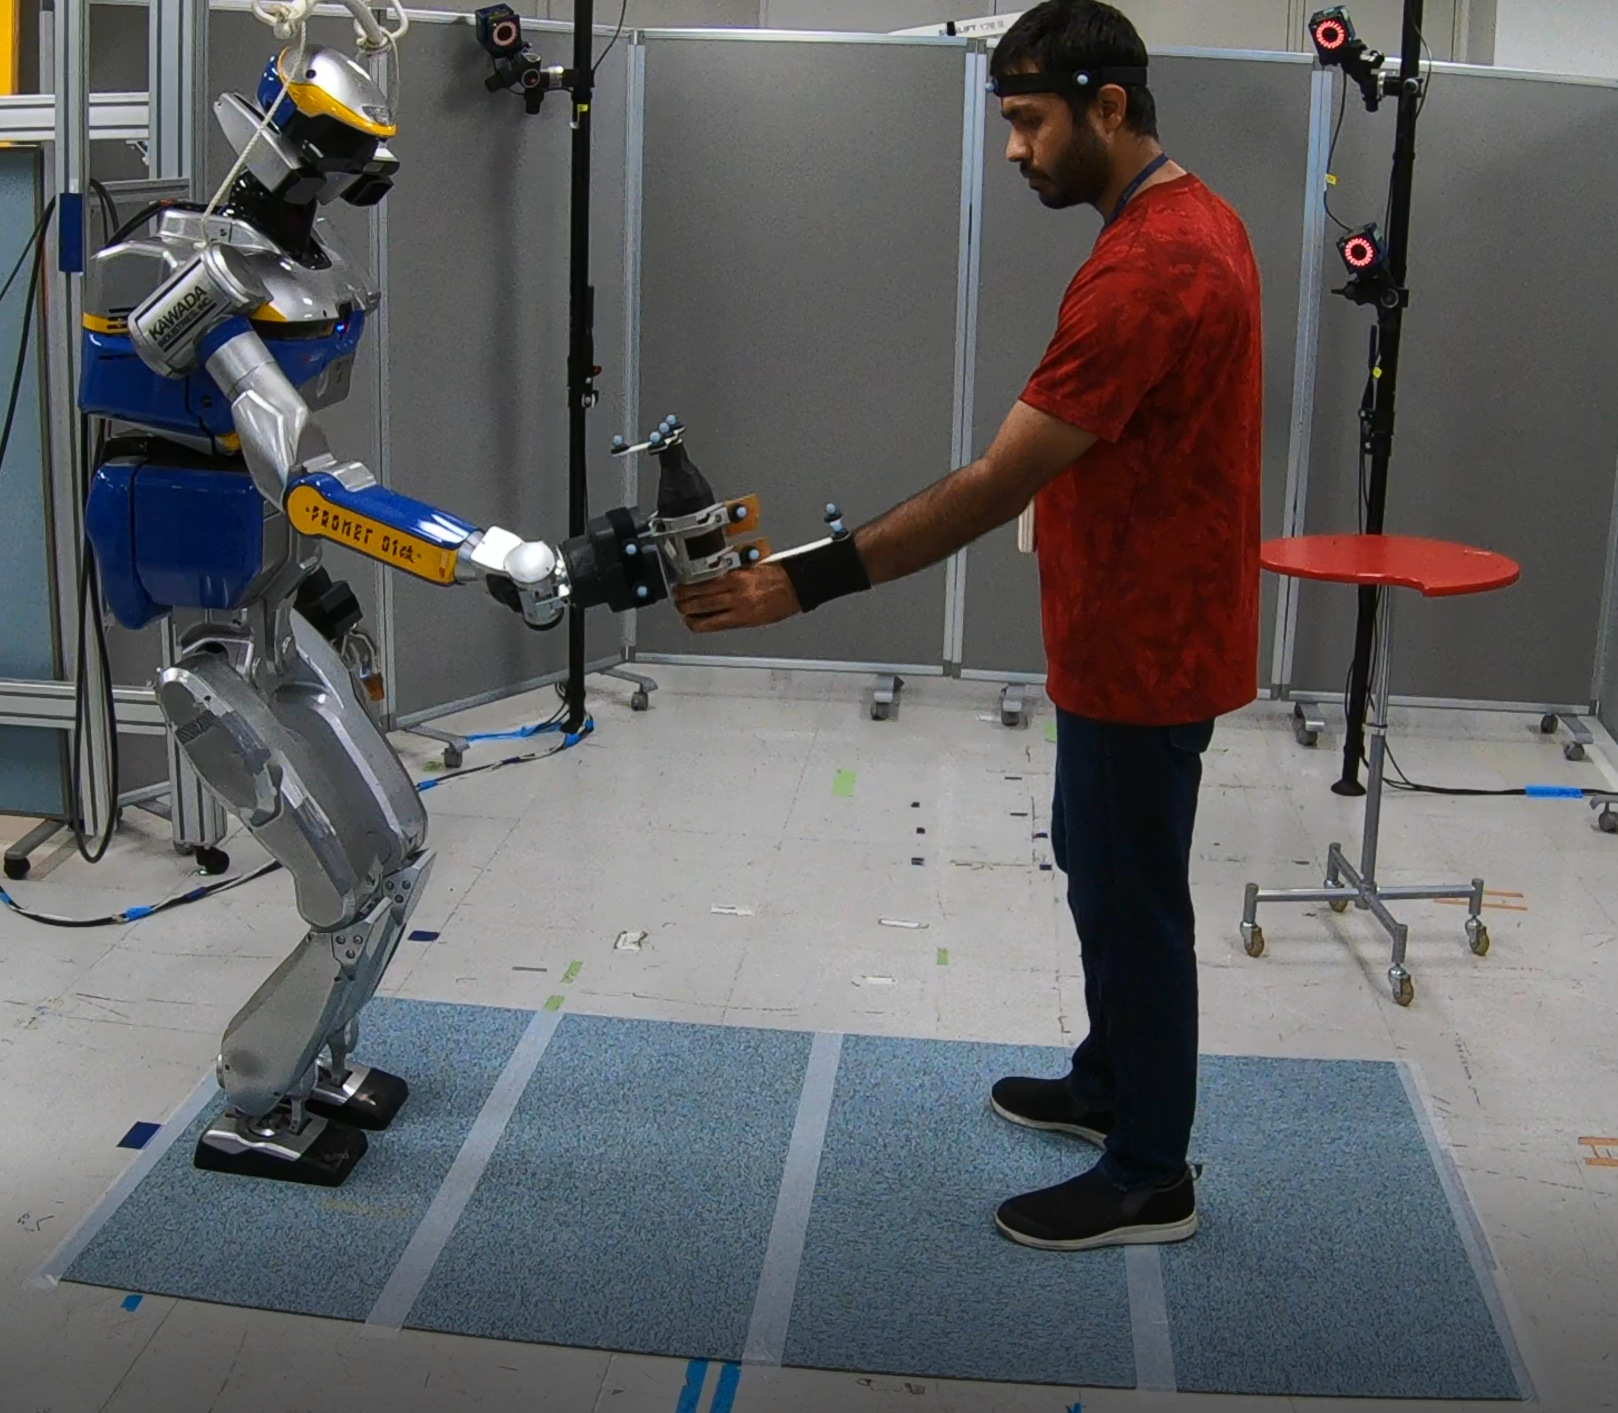
\includegraphics[width=.8\linewidth]{plots/c4-plots/hl-rr}}
	\caption{HRP-2Kai trying to grasp object using right end-effector.}
	\label{fig:markerEf1}
\end{figure} 

We explained further in detail in the subsection (\nameref{FSM}), but before that, we mention another (\nameref{surface wrench}) that we also utilize for closing gripper when the object is in the vicinity.



\subsection{Method 2: surface wrench}\label{surface wrench}

\begin{figure}[ht]
	\centering{\includegraphics[width=0.7\columnwidth]{plots/c4-plots/wrist-surface2}}
	\caption{Virtual intrinsic surfaces (green) on robot wrists.}
	\label{fig:wrist-surface2}
\end{figure}


Just by knowing the relative position of the object \texttt{w.r.t} the robot, end-effector gripper is not enough for safe and reliable object handover. As the lack of anthropomorphic hands and the visual features of the manipulative gripper can be intimidating to some humans. Therefore in conjunction to the mocap marker-based method mentioned earlier we also computed ${}^\text{surf}\vec{f}$, the \textit{gravity-free} force vector in the intrinsic surface frame $surf$ of the gripper (see Fig.~\ref{fig:wrist-surface2}). Let ${}^s\vec{f}\in F^6$ denote the \textit{gravity-free} spatial force vector in the local sensor frame $s$. Note that ${}^s\vec{f}$ has both force and couple components, but we were only interested in the force component. We can easily get the coordinate transformation between the surface frame and force sensor frame, knowing the body at which the force sensor is attached.

\begin{equation}\label{X_s_surf}
    {}^\text{surf}X_{s} = {}^\text{surf}X_{b} {}^{b}X_s
\end{equation}

where, $b$ denotes the body frame at which the force sensor is attached, in our case force sensor(s) are attached to the wrist(s) of HRP-2Kai.

One can generally obtain the transformation matrix for a force vector as explained in~\cite{featherstone2014rigid} if $X$ is responsible for coordinate transformation on motion vectors then using the equation (\ref{X*}), $X^{*}$ would do the same transformation on force vectors since both are related~\cite{featherstone2014rigid},

%%% check page 17-25
\begin{equation}\label{X*}
    X^{*} = X^{-T}
\end{equation}

therefore, force vector in the surface frame $surf$ can be obtained by utilizing equations (\ref{X*}) and (\ref{X_s_surf}), we get

% Dual Coordinates: page 9~\cite{featherstone2014rigid} $X^{*} f$, check page 246 as well
\begin{equation}\label{force surf}
    {}^\text{surf}\vec{f} = {}^\text{surf}X_{s}^{*} {}^s\vec{f}
\end{equation}

where, ${}^\text{surf}X_{s}^{*}$ is the transformation matrix for transformation of force vector from force sensor frame $s$ to gripper intrinsic surface frame $surf$. Finally we measure $\abs{{}^\text{surf}\vec{f}}$ (after removing initial offset) along the gripper's insertion ($z$)-axis, during the interaction between object and gripper just prior to handover during 1$^\text{st}$ \textit{sequence} and if the measured $\abs{{}^\text{surf}\vec{f}}$ is greater than 5N along with the outcome of equation (\ref{area}) then it is safe for robot to close the gripper and hence grasp the object. We further explained complete handover \textit{routine} utilizing above discussed methods in the next subsection (\nameref{FSM}).

\subsection{Finite state machine}\label{FSM}

\begin{figure}[hpt]
	\centering{\includegraphics[width=1\columnwidth]{plots/c4-plots/h-to-r.jpg}}
	\caption{human to humanoid object handover, t1 to t8 transition states.}
	\label{fig:h-to-r}
\end{figure}

The whole handover \textit{routine} is a continuous process but for clarity we have divided it into several transition steps of Finite State Machine (FSM)~\cite{johnson1968automatic}, also (see Fig.~\ref{fig:fsm}) for graphical implementation and Algorithm (\ref{interaction forces}) of (\nameref{handoverAppendix}) as well, the transitions between states are set to be continuous upon the success of previous transition. To understand the interaction forces model, let $\mathcal{\vec{F}}\in \mathbb{R}^3$ denote the current \textit{gravity-free} force sensor reading in the robot frame $\mathcal{R}$. During 1$^\text{st}$ \textit{sequence} of human to robot handover when human holds the object and starts to approach somewhere with the reachable workspace of robot to handover the object (see Fig.~\ref{fig:h-to-r}), in such a situation due to any acceleration of the robot end-effector while approaching towards the object, a wrist force sensor would only show readings due to the inertial forces~\cite{spong2008robot} that are acting on the robot end-effector, which we termed ${}^\text{zero}\vec{\mathcal{F}}$ as force sensor offset reading (see equation~\ref{Fzero}). Let ${}^\text{obj}\overline{\mathcal{F}}\in \mathbb{R}^3$ be the average of contact forces between the end-effector (gripper) and the environment (object) during the resting (${}^{\text{ef}}v=0$) period of robot end-effector along the $xyz$ axes and let ${}^\text{inert}\vec{\mathcal{F}}$ be the inertial force acting on the object due to the acceleration (lets call it ${}^{\text{ef}}a$) of robot end-effector when moving towards the predicted pose of human hand during the 2$^\text{nd}$ \textit{sequence} of handover as shown in (Fig.~\ref{fig:r-to-h}). Let ${}^\text{pull}\vec{\mathcal{F}}$ be the current \textit{minimum} interaction force exerted on the object by the human co-worker and sensed by the robot wrist force sensor while retreating the object during 2$^\text{nd}$ \textit{sequence} of robot to human handover and let ${}^\text{old}T$, ${}^\text{new}T$ $\in \mathbb{R}^3$ be the respective initial default hand-tuned and updated force thresholds. We now explain each state of FSM as shown in (Fig.~\ref{fig:fsm}).


\begin{figure}[hptb]
	\centering
	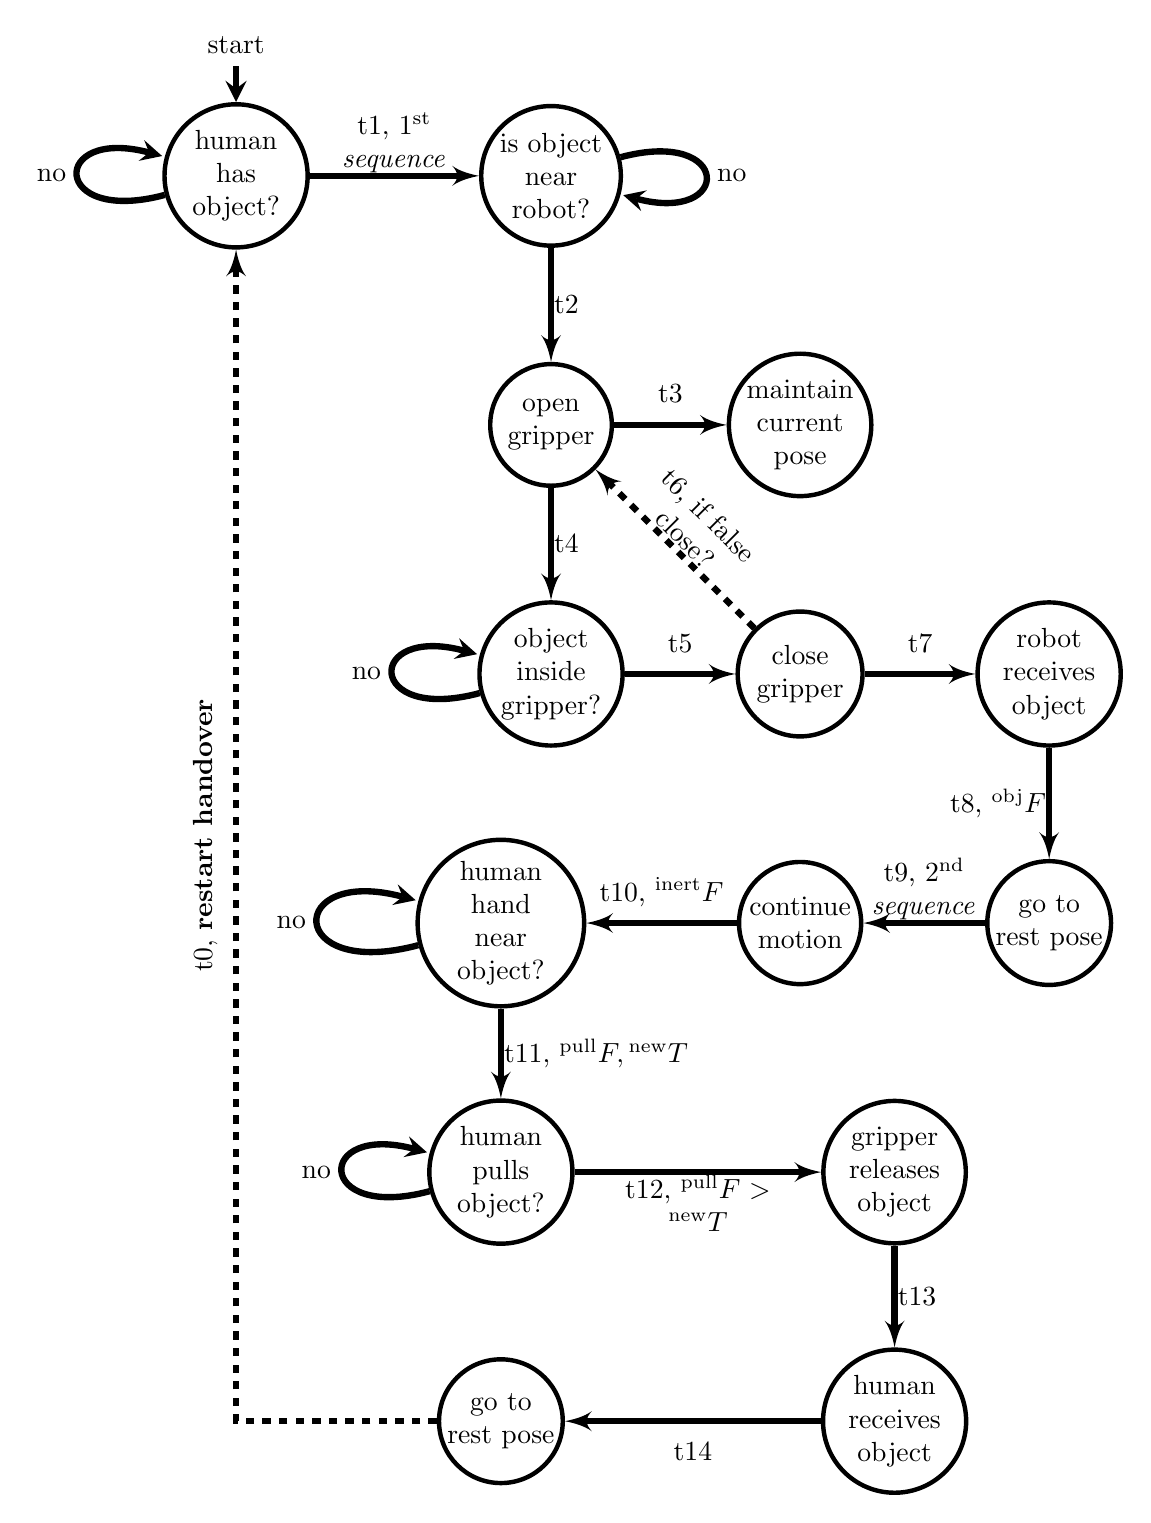
\begin{tikzpicture}[node distance=5cm, auto, scale = 1, ->,>=stealth, line width=2.3pt, kant/.style={text width=2cm, text centered, sloped}]
	\tikzstyle{cloud} = [draw,ultra thick, circle ,fill=white!20, text width=4em, text centered, node distance=9em, auto, inner sep=0pt, minimum height=1em]
	\tikzstyle{blank} = [circle ,fill=white!20, text width=5em, text centered, node distance=5em, auto, inner sep=0pt, minimum height=2em]
	\tikzstyle{line} = [draw, -latex', inner sep=0pt, minimum height=2em]
	
	\node[cloud,initial above] (human has object) {human has object?};
	\node[cloud, node distance=4cm] (human hand is near?) [right of=human has object] {is object near robot?};
	\node[cloud] (open gripper) [below of=human hand is near?] {open gripper};
	\node[cloud] (stop motion) [right of=open gripper] {maintain current pose};
	\node[cloud] (object inside gripper?) [below of=open gripper] {object inside gripper?};
	\node[cloud] (close gripper) [right of=object inside gripper?] {close gripper};
	\node[cloud] (robot has object) [right of=close gripper] {robot receives object};		
	\node[cloud] (go rest pose) [below of=robot has object] {go to rest pose};
	\node[cloud] (start motion) [left of=go rest pose] {continue motion};
	\node[cloud, node distance=3.8cm] (human hand is near again?) [left of=start motion] {human hand near object?};	
	\node[cloud] (pull handover object) [below of=human hand is near again?] {human pulls object?};
	\node[cloud, node distance=5cm] (open gripper release object) [right of=pull handover object] {gripper releases object};
	\node[cloud] (handover occurred) [below of=open gripper release object] {human receives object};
	\node[cloud, node distance=5cm] (go rest pose2) [left of=handover occurred] {go to rest pose};
	\node[blank] (blank)[left of = go rest pose2]{};
	
	\path[->] (human has object)  edge [loop left]   node  {no} ();
	
	\path [line] (human has object) edge     node[above, kant]{t1, 1$^\text{st}$ \textit{sequence}} (human hand is near?);
	
%	\draw[black,thick,->] (human hand is near?.90) node [above ]{no} arc  (0:240:6mm);
	  \path[->] (human hand is near?)  edge [loop right]   node  {no} ();
 
	
	\path [line] (human hand is near?) edge      node {t2} (open gripper);
	\path [line] (open gripper) edge              node {t3} (stop motion);
	\path [line] (open gripper) edge              node {t4} (object inside gripper?);
	
	\path [line] (object inside gripper?) edge   node {t5} (close gripper);
	 \path[->] (object inside gripper?)  edge [loop left]   node  {no} ();
	
	\path [line, dashed] (close gripper) edge          node [above, kant]{t6, if false close?} (open gripper);
	\path [line] (close gripper) edge         node {t7}(robot has object);
	\path [line] (robot has object)edge        node[left]{t8, ${}^\text{obj}F$} (go rest pose);
	\path [line] (go rest pose) edge           node [above, kant]{t9, 2$^\text{nd}$ \textit{sequence}} (start motion);
	\path [line]  (start motion)edge           node [above, kant]{t10, ${}^\text{inert}F$} (human hand is near again?);
	
	\path [line]  (human hand is near again?)edge  node {t11, ${}^\text{pull}F, {}^\text{new}T$}  (pull handover object);
	 \path[->] (human hand is near again?)  edge [loop left]   node  {no} ();
	
	\path [line]  (pull handover object)edge       node [below, kant]{t12, ${}^\text{pull}F >{}^\text{new}T$} (open gripper release object);
	\path[->] (pull handover object)  edge [loop left]   node  {no} ();
	
	\path [line]  (open gripper release object)edge  node {t13}(handover occurred);
	\path [line]  (handover occurred)edge           node {t14}(go rest pose2);
	\path [line, dashed]  (go rest pose2) -|       node [near end, above, rotate=90]{t0, \textbf{restart handover}}(human has object);
	
	\end{tikzpicture}
	\caption{Overview of human humanoid object handover Finite-State-Machine (FSM)}
	\label{fig:fsm}
\end{figure}


\begin{figure}[hpt]
	\centering{\includegraphics[width=1\columnwidth]{plots/c4-plots/r-to-h.jpg}}
	\caption{humanoid to human object handover t9 to t14 transition states.}
	\label{fig:r-to-h}
\end{figure}

\begin{enumerate}[start=0,label={\bf{t}\arabic*:}]

    \item $\norm{{}^h{P} - {}^\text{obj}{P}} < 0.02$\\
    We start FSM under the assumption that the human co-worker is already grasping the object, and he/she is ready with the intention of handover. ${}^h{P}$ is the position of point $A$ on the ${\bf L}$ shape body as the human hand marker position (see Fig.~\ref{fig:lshapes}).
    
    
    \item $\norm{{}^h{P} - {}^{\text{ef}}{P}} < 0.10$\\
    During 1$^\text{st}$ \textit{sequence} of handover \textit{routine}, i.e. human to robot object handover. We measure the relative position of human hand and robot end-effector mocap markers, the state transition is successful if the euclidean distance $d$ is less than 0.1 meters, where $d = \norm{{}^h{P} - {}^{\text{ef}}{P}}$. ${}^{\text{ef}}{P}$ is the average position of gripper tips marker ${}^\text{ga}P, {}^\text{gb}P$. 
    
    \item Open Gripper\\
    The robot opens the gripper and presents with its intention to grasp the object.
    
    \item $\norm{{}^h{P} - {}^{\text{ef}}{P}} \leq 0.05$, maintain current pose\\
    To avoid collision between robot end-effector and human hand we reduce the end-effector velocity (${}^{\text{ef}}v\simeq0$) when the interaction distance $d = \norm{{}^h{P} - {}^{\text{ef}}{P}}$ is less than 0.05 meters. We also measure ${}^\text{zero}\vec{\mathcal{F}}$ as force sensor offset during this time.
    
    \begin{equation}\label{Fzero}
    {}^\text{zero}\vec{\mathcal{F}} = {\vec{\mathcal{F}}}
    \end{equation}
    
    \item (${}^\text{surf}\vec{f}(z) \geq 5N) \quad $ \& $ \quad (f({}^\text{obj}\vec{P})  == 1$)\\
    We declare robot is ready to close the gripper when the object is inside gripper if output of equations (\ref{area bool},~\ref{force surf}) satisfy together.
    
    \item Close Gripper\\
    Let ${}^\text{close}\vec{\mathcal{F}}$ be the measured force reading at the timing of closing gripper.
        
    \begin{equation}\label{Fclose}
	    {}^\text{close}\vec{\mathcal{F}} = \vec{\mathcal{F}}
    \end{equation}
    
    Robot closes gripper; presumably, the object is grasped as well. However, it is easy to check whether the robot grasps the object or if it is a false close. It is safe to say that its a false close if output of equation (\ref{area bool}) is $0$, along with the condition $\norm{{}^\text{zero}\vec{\mathcal{F}}-{}^\text{close}\vec{\mathcal{F}}} \simeq{0}$, since these are same measured force sensor offsets. Therefore, in such scenario next transition state would be \textbf{t6} to open gripper and repeat, otherwise \textbf{t7}, as shown in (Fig.~\ref{fig:fsm}).
   
   \item Open Gripper due to false close, otherwise,
   
   \item This transition confirms that the robot receives the object and now the object \textit{mass} can be calculated based on the forces measured during previous states.
   
   \begin{equation}
   {}^\text{obj}\overline{\mathcal{F}} = \frac{1}{n}\sum_{i=1}^{i=n} \vert{ (\vert{\vec{\mathcal{F}}}\vert - \vert{{}^\text{zero}\vec{\mathcal{F}}}\vert) }\vert
   \end{equation}
   
   ${}^\text{obj}\overline{\mathcal{F}}$, is pure force sensor reading when ${}^{\text{ef}}a=0$ and object is grasped by the robot, $n$ is the low-level controller time-step counter that increments every $5$ ms (see subsection~\nameref{QPController}), before transitioning to next state, we intentionally stay on this state for 1 second i.e. until $i==200$ to measure the average of ${}^\text{obj}\vec{\mathcal{F}}$ over 200 samples. Finally, object $mass$ can be obtained using equation (\ref{obj mass}).
   
   \begin{equation}\label{obj mass}
   objMass = \norm{{}^\text{obj}\overline{\mathcal{F}}}/9.80665
   \end{equation}
   
   \item Go to rest pose \\
   Both human and robot return to their resting posture, with the robot carrying the object. This ends the 1$^\text{st}$ \textit{sequence} of handover.
   
   \item 2$^\text{nd}$ \textit{sequence} begins\\
   Robot to human object handover. The robot continues to predict human hand position and moves towards it when the human co-worker approaches somewhere within the robot's reachable workspace. During this time, we measure the ${}^\text{inert}\vec{\mathcal{F}}$ inertial force acting on the object due to the acceleration of end-effector.
   
   \begin{equation}
   {}^\text{inert}\vec{\mathcal{F}}  = objMass * {}^{\text{ef}}\overline{a}
   \end{equation}
   
   Where, ${}^{\text{ef}}\overline{a}$, is the average acceleration of the robot end-effector.
   
   \item $\norm{{}^h{P} - {}^{\text{ef}}{P}} < 0.05$\\
   Once again, we measure the relative position of human hand and robot end-effector mocap markers, the state transition is successful if the euclidean distance $d = \norm{{}^h{P} - {}^{\text{ef}}{P}}$ is less than 0.05 meters. That means human is ready with the intention to grasp the object.
   
   \item Human attempts to retrieve the object
   
   \begin{equation}
   {}^\text{pull}\vec{\mathcal{F}} = \vert{ (\vert{\vec{\mathcal{F}}\vert} - \vert{{}^\text{inert}\vec{\mathcal{F}}}\vert - \vert{{}^\text{zero}\vec{\mathcal{F}}}\vert) }\vert
   \end{equation}
   
   \begin{equation}
   {}^\text{new}\vec{T} = {}^\text{obj}\overline{\mathcal{F}} + {}^\text{old}\vec{T}
   \end{equation}
   
   where, ${}^\text{old}\vec{T}$ was hand tuned after several attempts with multiple objects. Default ${}^\text{old}\vec{T}$ values were set to $[6, 6, 6]$ N, after some preliminary trials. 
   
   \item Open Gripper, human grasps the object if both below conditions satisfy
   
   \begin{equation}\label{Fpull}
   \begin{cases}
   \norm{{}^h{P} - {}^\text{obj}{P}} < 0.02  \\
   {}^\text{pull}\vec{\mathcal{F}}\geq {}^\text{new}\vec{T}, & \lor x, \lor y, \lor z
   \end{cases}
   \end{equation}
   
   where, $\norm{{}^h{P} - {}^\text{obj}{P}}$ is again euclidean distance between human hand and object mocap markers.
   
   \item Object returns to the human co-worker, human retreats.
   
   \item End of 2$^\text{nd}$ \textit{sequence} of handover.\\
   Both human and robot returns to their resting posture, with human carrying the object (see Fig.~\ref{fig:halfsit}).
    
\end{enumerate}

Finally, this ends the object handover \textit{routine} between human and robot co-workers. Afterwards, we again repeat the handover \textit{routine}, starting with 1$^\text{st}$ \textit{sequence} of handover.



\section{Either hand generalized handover}\label{both hands individual}

As mentioned in an earlier section (\nameref{handover routine}), up till now we have discussed human-robot bi-directional object handover under the scenario where robot always uses its left end-effector, and human always uses his/her right hand. However unlike several handover studies in the past~\cite{cakmak2011human, medina2016human, huber2008Indus, kupcsik2016learning}, we can take the benefit of having a humanoid at our disposal; therefore we further generalize our human-humanoid bi-directional object handover \textit{routine} and extend it by exploiting either human left or right hand and similarly left or right end-effector of robot. Basically we extended our one-handed handover \textit{routine} into four possible scenarios (see Fig.~\ref{fig:handover scenarios}) such as,

\begin{enumerate}
	\item robot left end-effector $R_\text{efl}$ $\longleftrightarrow$ human right hand $H_r$
	\item robot left end-effector $R_\text{efl}$ $\longleftrightarrow$ human left hand $H_l$
	\item robot right end-effector $R_\text{efr}$ $\longleftrightarrow$ human left hand $H_l$
	\item robot right end-effector $R_\text{efr}$ $\longleftrightarrow$ human right hand $H_r$
\end{enumerate}


\begin{figure}[hpt]
	\centering
	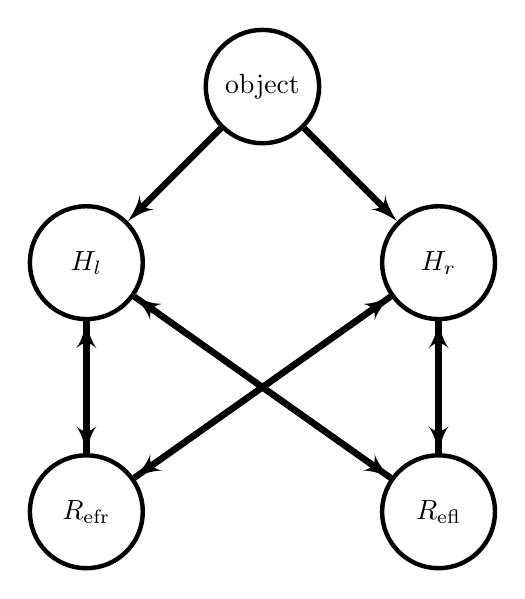
\begin{tikzpicture}[node distance=5cm, auto, scale = 1, ->,>=stealth, line width=2.3pt, kant/.style={text width=2cm, text centered, sloped}]
		\tikzstyle{cloud} = [draw,ultra thick, circle ,fill=white!20, text width=4em, text centered, node distance=9em, auto, inner sep=0pt, minimum height=1em]
		\tikzstyle{line} = [draw, -latex', inner sep=0pt, minimum height=2em]
		
		\node[cloud] (obj) {object};
		\node[cloud] (hl) [below left of = obj] {$H_l$};
		\node[cloud] (hr) [below right of= obj] {$H_r$};

		\node[cloud] (rr) [below of = hl] {$R_\text{efr}$};
		\node[cloud] (rl) [below of= hr] {$R_\text{efl}$};

		\path [line] (obj) edge  node[above, kant]{} (hl);
		\path [line] (obj) edge  node[above, kant]{} (hr);		
		
		\path [line] (hl) edge  node[above, kant]{} (rl);
		\path [line] (rl) edge  node[above, kant]{} (hl);
	
		\path [line] (hl) edge  node[above, kant]{} (rr);
		\path [line] (rr) edge  node[above, kant]{} (hl);
	
		\path [line] (hr) edge  node[above, kant]{} (rl);
		\path [line] (rl) edge  node[above, kant]{} (hr);
		
		\path [line] (hr) edge  node[above, kant]{} (rr);
		\path [line] (rr) edge  node[above, kant]{} (hr);

	\end{tikzpicture}
	\caption{Possible handover scenarios between human and humanoid.}
	\label{fig:handover scenarios}
\end{figure}


In this section we will only mention changes that need to be incorporated into the previous sections for the generalization and extension of previously stated handover \textit{routine} to cover above four possible scenarios (Fig.~\ref{fig:handover scenarios}). We mainly modify here parameters of FSM states during transitions {\bf t0, t1} and {\bf t10}, which are already discussed in detail (see subsection~\nameref{FSM}). Again we assumed a human is ready to handover the object if he/she is holding it in his/her either hand. We have also assumed that just like many humans, our robot also acts like a \textit{right-handed} `person', therefore robot right end-effector would get priority over left in case object is at relatively same distance from both end-effectors or in case where the handover predicted position is at or converging towards the centre of robot body. This hand preference is mainly due to a recent study~\cite{han2013quantifying}, which showed that right-handed people tend to prefer the right over left hand when they have the choice of pointing at a target location that is almost equally distant between both hands.


In this framework, the choice or preference of employing end-effector (either left or right) by the robot co-worker is based on the shortest relative distance of object to either human hand, which can be determined by using equation (\ref{human obj dist}) along with together the direction (mainly along $y$-axis) and shortest relative distance of \textit{that} active human hand with respect to both end-effectors, as per equations (\ref{human hand dir} and~\ref{robot obj dis}) respectively. For example, if human is holding object in his/her right hand ${}^\text{hr}{P}$ and if the estimated predicted position of his/her hand (see section~\nameref{prediction_model}) is converging somewhere in the negative $y$-coordinate space, then robot right end-effector ${}^\text{efr}{P}$ would be utilized to receive the object during handover as shown in (Fig.~\ref{fig:hr-to-rr}).


\begin{figure}[hpt]
	\centering{\includegraphics[width=0.7\columnwidth]{plots/c4-plots/hr-rr}}
	\caption{Object handover between human right hand and HRP-2Kai right end-effector.}
	\label{fig:hr-to-rr}
\end{figure}


\begin{equation}\label{human obj dist}
\centering
\begin{cases}
	\norm{{}^\text{hl}{P} - {}^\text{obj}{P}} < \norm{{}^\text{hr}{P} - {}^\text{obj}{P}}, & \text{human left hand (${}^\text{hl}{P}$)}  \\
	\\
	\norm{{}^\text{hl}{P} - {}^\text{obj}{P}} > \norm{{}^\text{hr}{P} - {}^\text{obj}{P}}, & \text{human right hand (${}^\text{hr}{P}$)}
\end{cases}         
\end{equation}


\begin{equation}\label{human hand dir}
\centering
\begin{cases}
\norm{{}^{h}{P}(y)} > 0.1,  &  \text{robot left end-effector (${}^\text{efl}{P}$)} \\
\\
\norm{{}^{h}{P}(y)} \leq 0.1,  &  \text{robot right end-effector (${}^\text{efr}{P}$)}
\end{cases}         
\end{equation}

\begin{equation}\label{robot obj dis}
\centering
\begin{cases}
\norm{{}^{h}{P} - {}^\text{efl}{P}} < \norm{{}^{h}{P} - {}^\text{efr}{P}}, &  \text{robot left end-effector (${}^\text{efl}{P}$)} \\
\\
\norm{{}^{h}{P} - {}^\text{efl}{P}} > \norm{{}^{h}{P} - {}^\text{efr}{P}}, &  \text{robot right end-effector (${}^\text{efr}{P}$)}
\end{cases}
\end{equation}


Where ${}^{h}{P}$ in equations (\ref{human hand dir} and~\ref{robot obj dis}) could be either of the human hand position depending upon equation (\ref{human obj dist}). However in cases where there is a switching of object in between human hands and within the 1$^\text{st}$ \textit{sequence} of handover, such as in some rare case human co-worker may decide to move the object from his/her left to right hand or vice-versa for any reasons, under those conditions we rely on the effect of \textit{hysteresis} for robot to decide whether it needs to switch end-effector or continue uninterruptedly. But note that we do not consider the problem of object handover in-between robot end-effectors, therefore once the object is being handed over to the robot co-worker, i.e. during 2$^\text{nd}$ \textit{sequence}, then the robot would not be able to switch its end-effector, however the human co-worker is still free to choose either of his/her hand to grasp the object back. Using the earlier example where human co-worker right hand has the object, and his/her position is converging somewhere in the negative $y$-coordinate space. While during the 1$^\text{st}$ \textit{sequence} of handover if human switches the object in-between his/her hand ---say from right to left hand, then by taking recent history (direction) of human hand into account we further utilize the outputs of equations (\ref{human hand dir} and~\ref{robot obj dis}) to measure change in the direction of human hand and its shortest relative distance from the end-effectors, and based on these observations robot decides to act accordingly. By exploiting \textit{hysteresis} effect, we make sure that robot does not respond abruptly to changes made by the human.


%\clearpage

\section{Bi-manual handover}\label{both hands together}

It is very natural between humans to use both hands to manipulate a heavy or large shape object to gain confidence and maintain stability during a physical interaction or even while performing a collaborative task. Using both hands together during handing over such an object to one another is no different. Similarly, in scenarios where the use of the single hand is not enough or feasible to perform safe and reliable handover of a large, heavy object between human and humanoid co-workers, then it should also be an obvious choice for the robot as well to use both hands together whenever necessary. 


Here, we extend the handover \textit{routine} under the scenario of bi-manual large object transfer between human and humanoid co-workers. We formulate this handover \textit{routine} in a manner such that human co-worker is allowed to use either or both hands to handover/receive the object to/from robot co-worker. However, the robot would always use both hands while receiving and returning of such object, given the physical, structural properties of the object.


\subsection{Handover object(s)}


\begin{figure}[hpt]
	\centering{\includegraphics[width=0.8\columnwidth]{plots/c4-plots/handoverPipe}}
	\caption{Hollow cylinder shaft as object for bi-manual handover between human humanoid. Subplot A) shows inner and outer radius of the hollow cylinder and placement of the $\bf L $ body shape with $o$. Subplot B) shows representation of our method to get the offset for safe handover location.}
	\label{fig:pipe_ex}
\end{figure}


The object(s) (two of them) we chose to handover between human-humanoid dyads are cylindrical (see Fig.~\ref{fig:pipe_ex}). We chose these objects purely for simplicity and demonstration purposes in this study. Though our handover model would practically work on several distinguishable objects as long as the object's basic physical, structural properties are known; however, the mass of the object is optional. The cylindrical structures we used are hollow yet quite rigid. The inner $r_i$ and outer $r_o$ radii for those two objects are \textins{$0.055$, $0.065$} m and \textins{$0.07$, $ 0.08$} m respectively, lengths $l$ are \textins{$0.90$, $ 0.12$} m, and the mass of objects are \textins{$0.40$, $1.1$} kg, again we don't need to know mass of object in advance as it can be computed during handover \textit{routine} when robot carries the object as already explained earlier in the subsection (\nameref{FSM}).


\begin{figure}[hpt]
	\centering{\includegraphics[width=0.7\columnwidth]{plots/c4-plots/robot_has_pipe}}
	\caption{HRP-2Kai using both end-effectors to manipulate handover object based on the human hand relative orientation.}
	\label{fig:pipe_ori}
\end{figure}


Here as well we have placed a ${\bf L}$ shape rigid body at the centre of the object as shown in (Fig.~\ref{fig:pipe_ex} and Fig.~\ref{fig:pipe_ori}) with respective $xyz$ local coordinate axes in local frame $o$ and are along the direction of robot frame axes. The object pose (position and orientation) is given by ${}^{o}{X}_M$ (see equation~\ref{X_M_o}). Also object orientation can be formulated similarly to human hand orientation, as explained earlier in section (\nameref{orientation_model}).


\subsection{Constraint motion}

Following is an overview of constraint motion during handover \textit{routine} using both hands and end-effectors.
\begin{compactitem}
	\item Human moves with the intention to handover the object.
	\item Both robot end-effectors approaches towards the object.
	\item Robot receives the object.
	\item Contacts are established between robot grippers and object surfaces.
	\item The contact constraint governs robot end-effectors motion under null velocity.
	\item Robot end-effectors follows the dominant human hand under the contact constraint.
\end{compactitem}

Here we approach differently during the 1${}^\text{st}$ and 2${}^\text{nd}$ \textit{sequence}s of handover. During the 1${}^\text{st}$ \textit{sequence} of object handover from human to humanoid, we predict and estimate both human hands positions individually along with estimating the object orientation. Specifically, we use unique \texttt{position} and \texttt{orientation} tasks (see subsection~\nameref{QPTasks}) to move each of the robot end-effector to the desired handover location. Once the object is handed over to the robot co-worker and after grasping it using both end-effectors, we remove the \texttt{position} and \texttt{orientation} tasks on one of the end-effector at the beginning of 2${}^\text{nd}$ \textit{sequence} because of the kinematic contact constraints (see subsection~\nameref{QPConstraints}) imposed by the object. 

Now we would first introduce contact surfaces and kinematic constraints before explaining the simultaneous motion of the robot end-effectors due to constraints imposed by the object during 2$^\text{nd}$ \textit{sequence} of handover \textit{routine}.

\begin{figure}[hptb]
	\centering{\includegraphics[width=1\columnwidth]{plots/c4-plots/grippers-intern}}
	\caption{Robot grippers with graspable internal surfaces.}
	\label{fig:gripper-intern}
\end{figure}


\paragraph*{Contact surface(s)} 

The contact surfaces or surface patches were initially defined on the palm of each gripper in advance. Grippers local frame are shown in (Fig.~\ref{fig:gripper-intern}). The contacts are established, when during the handover \textit{routine} the robot grasps the object and its grippers internal surface come in contact with the object's graspable surface. These contacts are necessary to move freely or limit the motion of end-effectors in one or more direction (3 \texttt{x} translation or 3 \texttt{x} rotation)~\cite{bouyarmane2018multi}. Thus robot may lose one or more degrees of freedom (DOF) in motion due to the constraints introduced by the object's body.


\paragraph*{Contact kinematics and constraint}

To allow the concurrent motion of the robot end-effectors and the object, contacts are defined as the kinematic constraints in the (\nameref{QPController}), specifically we used the \textit{fixed} contact mode, as defined by the~\cite{balkcom2002computing}, where all six degrees of freedom are constrained (no translation, no rotation at contact) which restricts and prevents any possibility of sliding motion between the robot end-effectors and the object. Lets consider $b_{l}$, $b_{r}$ and $b_o$ be the respective left, right end-effectors and object bodies and let $v_i$ be the $i$-th body velocity. Let $j_l$, and $j_r$ be the two joints under the kinematic constraint between these bodies. Such that, the relative joint velocities $v_\text{jl}$ and $v_\text{jr}$ between these bodies in contact would be given by the set of equations (\ref{joint_vel})~\cite{Featherstone:1987} and therefore the velocity constraints between these bodies would be given by the set of equations (\ref{vel_const}) \cite{ohwovoriole1980externsion} (see also subsection~\nameref{QPConstraints}). We later introduce this velocity constraint to the (\nameref{QPController}).

\begin{equation}\label{joint_vel}
\centering
\begin{cases}
v_\text{jl} = v_\text{bl} - v_\text{bo} \\
v_\text{jr} = v_\text{br} - v_\text{bo} \\
\end{cases}
\end{equation}

\begin{equation}\label{vel_const}
\centering
\begin{cases}
J_\text{lo}(v_\text{bl} - v_\text{bo}) = 0\\
J_\text{ro}(v_\text{br} - v_\text{bo}) = 0\\
\end{cases}
\end{equation}

where, $J_\text{ik}$ is the Jacobian matrix of all points of contact forces between $i$-th body and $k$-th body.


\paragraph*{1$^\text{st}$ \textit{sequence}: before object-robot contacts}

Under the handover \textit{routine} scenarios, we initiate handover 1$^\text{st}$ \textit{sequence} when human holds the object and start approaching somewhere within the reachable workspace of the robot — assuming that he/she is ready with the intention to handover the object to the robot. The human can grasp the object with any possible comfortable orientation using either left/right or both hands simultaneously and any place on the object's surface along its length. The only constraint we put while holding/grasping object was not to occlude the ${\bf L}$ shape body and mocap markers on it (see Fig.~\ref{fig:h-r-pipe-handover} for such possible pose(s)).


\begin{figure}[hptb]
%	\centering{\includegraphics[width=0.7\columnwidth]{plots/c4-plots/h-r-pipe-handover}}
	\centering{\includegraphics[width=0.7\columnwidth]{plots/c4-plots/h-r-pipe-handover1}}
	\caption{Bi-manual object handover between human and humanoid using both human hands and both end-effectors.}
	\label{fig:h-r-pipe-handover}
\end{figure}

Compared to the one-handed handover scenario, which was discussed in previous section (\nameref{both hands individual}), here during human to robot co-worker object handover \textit{sequence} instead of just predicting human hand positions individually like earlier, we also measure the Euclidean distances of each human hand on the object's surface \texttt{w.r.t} the object's centre using the following set of equations (\ref{hand rel pos on obj}). These distances act as an offset correction to the predicted positions of human hands, along the length of the object. These offsets are essential as they allow the robot to find safe and optimum positions on the object's surface to grasp. Also, while making sure end-effectors stay quite away from the human hands occupied the object's surface (see Fig.~\ref{fig:h-r-pipe-handover}). Moreover, it avoids any possible head-on collision between the end-effectors and the human hands when the robot tries to approach and grasp the object.


Initially, we predict and estimate human hand positions by utilizing previously discussed prediction model from section (\nameref{prediction_model}). Given the object shape and its structural properties (in our case length of cylindrical shaft), the offsets along object's length can be calculated using set of equations (\ref{hand rel pos on obj}) in the object local frame $o$ (see Fig.~\ref{fig:pipe_ex} B) from the center in both directions. This offset is then further transformed into the robot frame and finally added to the already predicted position of the human hands \texttt{w.r.t} robot end-effectors using equation (\ref{offset_transform}).



\begin{equation}\label{hand rel pos on obj}
\centering
\begin{cases}
a = \norm{{}^\text{obj}{P} - {}^{h}{P}} & \text{}  \\

b = \abs{l/2 - a}  & \text{} \\
\\
{}^\text{off}{d} = \pm 2*a/3 &  \text{if} \; a \geq b \; $ \& $ \; a\leq l/2\\

{}^\text{off}{d} = \mp 2*b/3 &  \text{if} \; a < b \; $ \& $ \; a\leq l/2\\
\end{cases}
\end{equation}

where, ${}^\text{obj}{P}$ is the centre position given by the mocap marker at its centre, $a$, $b$ and ${}^\text{off}{d}$ are the euclidean distances, which provides grasped location of human hands on the object surface from its centre. Using this crucial information robot can estimate possible points on the object's surface, which are available to be grasped during the handover. Here, $h$ in ${}^{h}{P}$ represents either left $H_l$ or right $H_r$ human hand and the sign of ${}^\text{off}{d}$ depends on the choice of left or right human hand (see Fig.~\ref{fig:pipe_ex} B). Let $\hat{u} = \{0, 1, 0\}$ be the free unit vector along the length of the object, i.e. along the $o_y$-axis of local frame $o$, therefore offset position vector in object frame would be given by


\begin{equation}
	{}^\text{off}{P}_{o} = {}^\text{off}{d} \: \hat{u}  =  \{0, {}^\text{off}{d}, 0\}
\end{equation}


We know for sure that without these offsets, robot end-effectors would inevitably collide with the human hands. Since our prediction model is estimating and predicting the positions of both human hands. Therefore, we need to introduce these offsets in the predicted positions of human hands relative to robot end-effectors. We start by measuring these offsets continuously and from the beginning of handover $\textit{sequence}$. This allowed the robot to adjust while approaching the object, depending on the human hands grasped location on the object's surface. We can obtain the modified predicted positions based on these offsets using Pl\"ucker transformation. We transformed offset position ${}^\text{off}{P}_{o}$ from object frame to mocap frame ${}^\text{off}{P}_{M}$ by below equation (\ref{offset_transform}). Please note, above offset correction method is also valid during the 2$^\text{nd}$ \textit{sequence} of handover when robot holds the object and approaches towards the human decided handover location.


Note here, we considered predicted position of the human hand, but to relatively orient robot end-effectors, we considered the orientation of object but not the human hand(s). In this example of a cylindrical object, the orientation of human hand and object is similar however to generalize this for other possible distinguishable shape objects; it is crucial to consider object's orientation instead of the human hand. As for the other shape objects relative human hand's orientation to grasp the object may not be feasible to perform by the robot. 

%\begin{equation}\label{offset_transform}
%{}^\text{off}{X}_{M} = {}^\text{off}{P}_{o} {}^{o}\mathcal{O}_M
%\end{equation}

\begin{equation}\label{offset_transform}
{}^\text{off}{X}_{M} = 
{}^\text{off}{P}_{o}
 \left[\begin{array}{cc}
{}^{o}\mathcal{O}_M & {}^{h}\mathcal{P}_M(i_\text{predict})
\end{array}\right]
\end{equation}


where, ${}^{o}\mathcal{O}_M$ provides the orientation of object in the mocap frame (see equation~\ref{X_M_o}) and ${}^{h}\mathcal{P}_M$ is the predicted position of human hand(s). Finally, using equation (\ref{offset_transform}), we can replace translation and orientation components of ${}^{h}{X}_M$ in the equation (\ref{X_ef_ht}) with ${}^\text{off}{X}_{M}$, therefore new pose of the handover location relative to the robot end-effectors would be given by

\begin{equation}
	{}^{\text{off}}{X}_{\text{ef}} =  {\bf{}^{\text{\bf off}}{X}_M}  {}^{M}{X}_R {{}^{\text{ef}}{X}_R}^{-1}
\end{equation}
%	{}^{h}{X}_{\text{ef}}(\text{off}) =  {\bf{}^{\text{\bf off}}{X}_M}  {}^{M}{X}_R {{}^{\text{ef}}{X}_R}^{-1}


Finally, at the handover location, we measure the $\abs{{}^\text{surf}\vec{f}}$ (after removing initial offset) forces along the both gripper's insertion ($z$)-axes during the interaction between object and gripper just before handover. Handover occurs when $\abs{{}^\text{surf}\vec{f}}$ exceeds 5N on both end-effectors along with the set of following conditions in equation (\ref{min_posErr_vel}) satisfy for both robot end-effectors.



\paragraph*{2$^\text{nd}$ \textit{sequence}: after object-robot contacts}

So far we have discussed estimating and predicting object handover pose for the robot end-effectors during the 1${}^\text{st}$ \textit{sequence} of handover \textit{routine}. Up till now, each robot end-effector motion was controlled by its own \texttt{position} and \texttt{orientation} task. During the 2$^\text{nd}$ \textit{sequence} of handover \textit{routine} after the contacts have been established between the robot grippers and the object surfaces. Also, because of the introduction of kinematic constraints imposed by the object on the end-effectors, the robot cannot move its end-effectors individually. The successive motion of the end-effectors is therefore now governed by the \texttt{contact constraint} that we introduce to the robot's low-level QP controller. This constraint maintains the contacts between the object and the robot grippers surfaces all the time and the concurrent motion of the end-effectors is made possible by targeting a null velocity constraint with the target objective $\mathscr{I}_\text{contact}=0$ at the contact joints between the object and the end-effectors, see equation (\ref{vel_const}). The \texttt{contact constraint} is already explained at the beginning of this section and also in the subsection (\nameref{QPConstraints}).

As already mentioned earlier, the human co-worker is allowed to use either (both) hand(s) to handover/receive the object to/from robot co-worker. Therefore, when the human starts approaching somewhere within the reachable workspace of the robot to receive the object. We utilized equation (\ref{robot_rel dis}) to select the dominant human hand, mainly by measuring the relative distances between the robot end-effectors and the human hands. We check this condition only once at the beginning of the 2$^\text{nd}$ \textit{sequence} of handover \textit{routine} after the human hand(s) arrive within the reachable workspace of the robot.

\begin{equation}\label{robot_rel dis}
\centering
\begin{cases}
\norm{{}^\text{hr}{P} - {}^\text{efl}{P}} < \norm{{}^\text{hl}{P} - {}^\text{efr}{P}}, &  \text{robot left end-effector (${}^\text{efl}{P}$)} \\
\\
\norm{{}^\text{hr}{P} - {}^\text{efl}{P}} > \norm{{}^\text{hl}{P} - {}^\text{efr}{P}}, &  \text{robot right end-effector (${}^\text{efr}{P}$)} \\
\end{cases}
\end{equation}

Where, ${}^\text{hl}{P}$ and ${}^\text{hr}{P}$ are the position vectors of the respective left and right human hand. Depending on the choice of the dominant human hand, for example, if the left human hand is selected then we remove the \texttt{position}, and \texttt{orientation} tasks of the left end-effector and therefore the motion of this end-effector is now governed using the \texttt{contact constraint} by targeting the null velocity. By doing this, the robot right end-effector would lead the motion by predicting and estimating the pose of the dominant human hand. The problem of predicting and estimating human hand pose can now be treated similarly to the one-handed handover \textit{routine} as mentioned in the section (\nameref{both hands individual}). Please note, set of equations (\ref{hand rel pos on obj}) is also valid to calculate the offset position of end-effector when robot predicts and approaches towards the handover location chosen by the dominant human hand. We just need to replace the human hand position vector ${}^{h}{P}$ with the end-effector position vector ${}^{\text{ef}}{P}$. Where $\text{ef}$ in ${}^{\text{ef}}{P}$ is either left $\text{efl}$ or right $\text{efr}$ end-effector.


Finally, a handover occurs when the set of conditions in the equation (\ref{Fpull}) satisfy for both end-effectors (see~\nameref{FSM}). Note that the conditions in the equation (\ref{Fpull}) are valid only if a human tries to pull the object from the robot. After the robot grippers release the object, we also remove the null velocity \texttt{contact constraint} between the end-effectors and the object surfaces, and add again the previously removed \texttt{position} and \texttt{orientation} tasks to that end-effector. This completes bi-manual handover \textit{routine}.

%\clearpage

\section{Locomotion and handover}\label{locomotion}

A broad general definition of locomotion describes it as an ability to move from one place to another, that could be achieved either by walking, running, jumping and more. Though we are mainly interested in the walking locomotion of a \textit{floating} base robots such as our HRP-2Kai in the context of the object handover between human and robot co-workers. However, after a thorough search of state-of-the-art research in the related field, none of the previous work on the human-robot dyad considered object handover and `walking' in a single framework using a \textit{biped} humanoid platform such as HRP-2Kai. Therefore in order for the robot to be sufficiently proactive, we believe it is essential to consider the possibility of a robot taking a step or two to handover or exchange an object with the human co-worker, in scenarios where short-distance travel is required, to eventually extend robot's reachable workspace. Note that we consider the problem of taking a few steps to handover/receive the object rather than motion planning and navigation.

Some previous studies on human-human dyad object handover have demonstrated that we humans are surprisingly able to predict where our partner would handover an object, often without an explicit communication~\cite{kato2018humans, kato2019handovers}. However we came across one of such study~\cite{hansen2017human}, results of which had shown that we humans often handover an object at the middle of our interpersonal distances~\cite{hall1966proxemic, strabala2013toward}.

Up till now, we formulated our handover problem under the scenario that both human and especially robot co-worker base (feet) are stationary on their respective position in the world frame, such that object handover can happen just by extending their arms. Next in this section, we further extended our handover problem and added another dimension in which robot takes a step(s) (we call it \textit{step-walk}) to handover or receive the object from the human co-worker based on the interpersonal distance between them. We have tested this scenario during both when human-robot dyad uses either one hand or both hands simultaneously.


\subsection{Walking pattern generator}

Though there are many state-of-the-art methods available to generate walking pattern for humanoids, however in this study for step-walk locomotion, we primarily chose to adopt walking pattern generator (WPG) based on the Linear Inverted Pendulum Mode (LIPM) which was designed and tested in our group~\cite{ kajita20013d, caron2016humanoids} along with its native stabilizer~\cite{kajita2010biped, caron2018stair}. 

The goal of WPG is to generate the on-line trajectory $P_G(t)$ of the Center of Mass (CoM) of the robot, while all-time maintaining the Zero Momentum Point (ZMP) $P_Z(t)$ of the robot within the support polygon. This support polygon is usually defined by the contact points between the robot (feet) and the environment (floor). During Double Support Phase (DSP) --- when both feet are in contact with the ground, the contact surface corresponds to the convex hull of all possible (flat) ground contact points. While During the Single Support Phase (SSP) --- when one foot is above the ground (swing state), then this contact surface lies below the robot foot which supports its weight. 

In general, WPG provides CoM trajectory $P_G(t)$ and also the trajectory of an angular-momentum $L_c(t)$, however, when considering $L_c = 0$, this model can be reduced to a single output of CoM, and the resulting model is known as Inverted Pendulum Mode. While if walking is under the assumption of a horizontal flat surface (as in our handover problem) such that CoM height remains constant, then this model can be further simplified to Linear Inverted Pendulum Mode, as given by equation (\ref{wpg}). LIPM establishes a relationship between  ZMP and CoM of the pendulum, resulting in a dynamical system with CoM jerk as an input to the system. The desired ZMP trajectory can, therefore, we obtained by appropriately computing CoM jerk. Moreover, to ensure the balance of biped robot while walking, WPG task is to minimize the error between the CoM velocity and a reference velocity (one angular velocity and two translation velocities), also to minimize CoM jerk while respecting the constraints on the robot ZMP.



\begin{equation}\label{wpg}
P_Z =  P_G - \frac{h}{g} \ddot{P_G}
\end{equation}

where $g$ is gravity, $h$ is the constant height of CoM in equation (\ref{wpg}).

\begin{figure}[hpt]
	\centering
	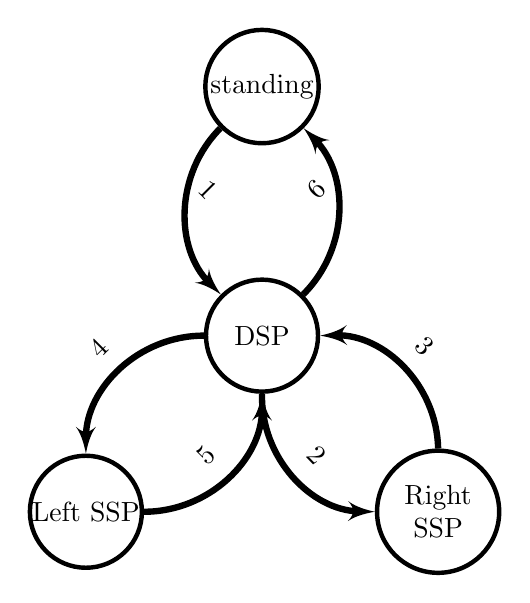
\begin{tikzpicture}[node distance=5cm, auto, scale = 1, ->,>=stealth, line width=2.3pt, kant/.style={text width=2cm, text centered, sloped}]
	\tikzstyle{cloud} = [draw,ultra thick, circle ,fill=white!20, text width=4em, text centered, node distance=9em, auto, inner sep=0pt, minimum height=1em]
	\tikzstyle{line} = [draw, -latex', inner sep=0pt, minimum height=2em]
	
	\node[cloud] (st) {standing};
	\node[cloud] (d) [below of = st] {DSP};
	\node[cloud] (l) [below left of  = d] {Left SSP};
	\node[cloud] (r) [below right of = d] {Right SSP};
		
	\path [line, bend right = 45] (st) edge  node[above, rotate=-45]{1} (d);
	
	\path [line, bend right = 45] (d) edge  node[above, kant]{2} (r);
	\path [line, bend right = 45] (r) edge  node[above, rotate=-45]{3} (d);

	\path [line, bend right = 45] (d) edge  node[above, rotate=45]{4} (l);	
	\path [line, bend right = 45] (l) edge  node[above, kant]{5} (d);
	
	\path [line, bend right = 45] (d) edge   node[above, rotate=45]{6} (st);
	
	\end{tikzpicture}
	\caption{Walking state machine with standing phase, single support phase (SSP) and double support phase (DSP).}
	\label{fig:wpg_FSM}
\end{figure}


In this study, the number of footsteps (two left and two right), length of footsteps, duration of single support, double support phases and swing height in WPG were predefined for robot during forward and backward step-walk. The WPG can be implemented using three phases of FSM (walking state machine) ---standing phase, double support phase and single support phase as illustrated in (Fig. \ref{fig:wpg_FSM} and Fig. \ref{fig:fwdWalk}).  We mentioned the parameters to control WPG in the (Table.~\ref{wpgParam}).


\begin{figure}[hptb]
	\centering{\includegraphics[width=\columnwidth]{plots/c4-plots/fwdbottom.jpg}}
	\caption{Bottom view of forward step-walk (4 footsteps) states of WPG: with starting phase Standing ---> DSP ---> Right SSP ---> DSP ---> Left SSP ---> Standing.}
	\label{fig:fwdWalk}
\end{figure}


\begin{table}[hbt]
	\caption{WPG parameters.}
	\label{wpgParam}
	\begin{center}
		\begin{tabular}{|c | c|}
			\hline
			{\bf Parameters} &  {\bf Values} \\ 
			\hline
			Total footsteps & 4\\
			\hline
			Footstep length & 0.2 meters\\
			\hline
			Swing height & 0.05 meters\\
			\hline
			SSP duration & 0.8 seconds\\
			\hline
			DSP duration & 0.2 seconds\\
			\hline
			Step-walk duration & 4.2 seconds\\
			\hline
		\end{tabular} 
	\end{center}
\end{table}




\subsection{Step-walk}

As said above, the moment at which this step-walk should be triggered depends on the interpersonal distance between human and robot co-worker bodies and along with the height of active human hand ($ {}^{z}H  = {}^{h}\mathcal{P}_M(z)) $ (object carrying/receiving hand). The interpersonal distance $ D $ (\ref{D}) is calculated between the human co-worker body position $ {}^{b}{H} $ and the robot co-worker body position $ {}^{b}{R} $ in the ${\bf X}$-coordinate (walking direction) of world frame. We get the robot body position by using \texttt{CoM} task (see~\nameref{QPTasks}), and as mentioned earlier, three mocap markers were placed on the head of the human co-worker to get his/her body position. These three markers make up a circle in $xy$-plane such that the centre of the circle is considered as the human co-worker body position. We remind again that we formulated the problem with a common origin {\it O}, therefore $\mathcal R \equiv M$ (both frames are located between the feet of robot HRP-2Kai).

\begin{equation}\label{D}
	D = \abs{{}^{b}{H} - {}^{b}{R}}
\end{equation}

Initially, the problem of handover was formulated under the scenario that both human and robot co-worker feet are stationary on their respective position in the world frame; therefore the object handover can happen just by extending their arm(s) and end-effector(s) respectively. However, with an exception that human co-worker is allowed to move nearer to the robot co-worker if needed. The initial interpersonal distance $ {}^{i}D $ between the human and robot co-workers bodies were approximately kept $1.2$ meters, such that object handover is possible as long as equations (\ref{reachable} and \ref{Di_range}) satisfy,

\begin{equation}\label{Di_range}
	0 <= {}^{i}D <= 1.2
\end{equation}

Though, now with the possibility of taking few step(s), our previous handover \textit{routine} can be extended further to some possible scenarios (within and beyond its initially defined reachable workspace) where an object handover could occur between human and humanoid, either using one hand or both hands together, even when human co-worker is out of robot's reachable workspace in the direction of $\bf{X}$-axis. 

The key idea here is to trigger the step-walk when human co-worker goes beyond the robot co-worker's reachable workspace (stepping backwards) and presents its intention to handover/receive the object. The intention of human co-worker is established when the condition (\ref{triggerWalk}) satisfy followed by the condition (\ref{aboveWaist}) i.e.  (\ref{triggerWalk}) $\&$ (\ref{aboveWaist}).


\begin{equation}\label{triggerWalk}
		125\%({}^{i}D) <= D <= 150\%({}^{i}D)
\end{equation}

\begin{equation}\label{aboveWaist}
		{}^{z}H >= waistHeight
\end{equation}

where, $ waistHeight $ is the height of respective human co-worker. Also note that $ {}^{z}H $ is not just any human hand but the active human hand height which either holds the object during 1$ {}^\text{st} $ \textit{sequence} or approaches towards the object to grasp it during 2$ {}^\text{nd} $ \textit{sequence} of a handover \textit{routine} as shown in (Fig. \ref{fig:handoverWalk}).


\begin{figure}[hptb]
	\centering{\includegraphics[width=0.7\columnwidth]{plots/c4-plots/handoverWalkOneHand}}
	\caption{Object handover between human and humanoid co-worker when robot takes a forward step-walk while attempting to grasp the object.}
	\label{fig:handoverWalk}
\end{figure}

%\clearpage

\section{Handover task protocol}

The handover task protocol is an emblem of our bi-directional object handover problem between human and humanoid co-workers. It consists of all the models and methods that we have presented so far. (\nameref{prediction_model}) for predicting and estimating the handover location. (\nameref{orientation_model}) for estimating the orientation of robot end-effector(s), relative to the orientation of an object or active human hand during handover. (\nameref{interaction model}) for minimizing the forces during the handover of an unknown mass object.

Moreover, when considering step-walk, the (\nameref{handover routine}) can be performed under four possible cases (see Table.~\ref{walkTable}) in which an object handover could occur between human and humanoid, either when during (\nameref{both hands individual}) or (\nameref{both hands together}) scenarios.

\begin{table}[hbt]
	\caption{Possible object exchange cases during the \textit{sequence}s of a handover \textit{routine}.}
	{During both \textit{sequence}s, human co-worker can handover the object while staying at their starting position or first take a step backward and then handover the object.}
	\label{walkTable}
	\begin{center}
		\begin{tabular}{| c | c|}
			\hline  
			{\bf 1${}^\text{st}$ \textit{sequence}} & {\bf 2${}^\text{nd}$ \textit{sequence}} \\ 
			\hline			
			stays &  stays  \\ 
			\hline			
			stays &  steps backward  \\
			\hline			
			steps backward & stays  \\ 
			\hline			
			steps backward & steps backward  \\ 
			\hline 			
		\end{tabular} 
	\end{center}
\end{table}

Within the handover task protocol, each trial of handover \textit{routine} starts from an initial posture, standing still with both hands down as shown earlier in (Fig.~\ref{fig:halfsit}), such that it must satisfy the condition (\ref{safezone}). 

\begin{equation}\label{safezone}
D > 150\% ({}^{i}D) 
\end{equation}


Afterwards, the trial begins when the human co-worker moves to a `starting position' (\ref{D_range}), from there it is up to human co-worker, whether he/she chooses to exchange (handover/receive) object from that stationary position or take a step backward, while at the same time raise his/her active hand, which results in signaling the robot to trigger the step-walk and eventually exchange the object with the human co-worker as per the conditions (\ref{triggerWalk}) $\&$ (\ref{aboveWaist}). Note that we utilize the fundamentals of hysteresis such that robot would trigger forward step-walk only when the conditions are valid in following mentioned order (\ref{safezone}) $\&$ (\ref{D_range}).


\begin{equation}\label{D_range}
0 <= D <= 1.2
\end{equation}


The step-walk is triggered when $ 125\%({}^{i}D) <= D <= 150\%({}^{i}D) $, where $ \max({}^{i}D)  == 1.2 $, while at the same time $ {}^{z}H $ is above human co-worker's waist. This basically agrees with our assumption that human co-worker is ready with the intention to handover/receive the object.

Finally, once the object handover has occurred, the robot co-worker needs to go back to its initial starting position, such that it requires to take backward step-walk to complete the handover \textit{sequence}. For simplicity, we have coupled the backward step-walk with the forward step-walk; therefore, backward step-walk is triggered only when the robot had taken forward step-walk. We trigger the backward step-walk, once the object is fully grasped by the robot co-worker (1$ {}^\text{st} $ \textit{sequence}), as stated by the transition states \textbf{t7} and \textbf{t8} of (\nameref{FSM}) or by the human co-worker at the end of (2$ {}^\text{nd} $ \textit{sequence}), as stated by the transition states \textbf{t12} and \textbf{t13}, then the robot safely return its end-effector(s) to a relax/initial posture and walks back to where it started. This lets completion of one trial of a handover \textit{routine}.


\section{Discussion}

To summarize this chapter, we introduced a framework to solve the problem of intuitive and proactive bi-directional object handover between a human and a biped humanoid co-worker dyad using whole-body control and locomotion. This handover framework has been implemented and tested on a real HRP-2Kai. Here we designed models to answer three important questions ---when (\textit{timing}), where (\textit{position in space}) and how (\textit{orientation and interaction forces}) of the handover \textit{routine}. By addressing the common key features of object handover between human and robot dyad ---the \textit{timing}(s) and overall duration of handover, the \textit{pose} of handover and the \textit{magnitude} of the interaction forces between human hand(s) and robot end-effector(s).


During the trials of a handover \textit{routine}, we found that our (\nameref{prediction_model}) is able to predict the human hand position such that robot is able to proactively plan its end-effector's motion and arrive at the human chosen handover location approximately at same time as human co-worker, both during the 1$ {}^\text{st} $ \textit{sequence}s and 2$ {}^\text{nd} $ \textit{sequence}s. This lead to an overall reduction in handover trial duration, thanks to the approximate prediction and estimation of handover location in advance. The behaviour of our prediction model can be tuned by two initially required constant time periods, $i_\text{observe}$ and $i_\text{predict}$, though at the moment we did not test its performance thoroughly. The values of  $i_\text{observe}$ and $i_\text{predict}$ were set to $ 20 $ ms and $ 200 $ ms respectively in the preliminary tests.

However, predicting handover location alone is not enough when robot co-worker is unaware of the grasp configuration that is required to handover the object. Also to keep in mind the comfort and requirement of the human co-worker~\cite{aleotti2012comfortable}, it is pivotal for the robot to be able to find the most appropriate configuration to grasp (as \textit{receiver}) or release (as \textit{giver}) the object. Moreover, according to \cite{cakmak2011human}, we humans prefer the handover of an object in its default orientation. Therefore, we mainly chose to handover the object in which it is most commonly being grasped hence the default orientation. We proposed a method to get the desired object grasping orientation of robot end-effector either by considering the relative orientation of the active human hand or the object itself in (\nameref{orientation_model}). The only limitation of this model is its dependency on the position of $ {\bf L} $ shape mocap markers, that is attached to the object (1$ {}^\text{st} $ \textit{sequence}) and active human hand wrist (2$ {}^\text{nd} $ \textit{sequence}). Another thing to note, in this study, we only considered class of rigid basic straight shape objects (bottle or pipe); however, it is possible to further generalize this method to other classes (compound shapes) of objects given the object physical, structural properties in advance. Because by knowing the object shape, $ {\bf L} $ body can be placed accordingly and offsets can be created for safer handover between human and robot co-workers as discussed in section (\nameref{both hands together}). The model is adaptable to objects of different mass within consecutive trials.


Another solution that we proposed here using (\nameref{interaction model}) is related to the \textit{timing} of grasping and releasing the object while at the same time minimizing the \textit{magnitude} of forces during the release of the object in such interactions. We designed a model of interaction forces using (\nameref{FSM}) which enables the robot end-effector to interact with the object independent of the knowledge of its mass in advance. We proposed two methods within this model, in first method we made sure that robot grasps/releases the object only when active human hand is within its gripper's graspable space using the mocap markers position and in second method we established the intention of the human co-worker to handover/receive the object by measuring the offset free-acting force on the intrinsic surface of the gripper along its insertion ($z$)-axis at the time of contact. Moreover, during the 2$ {}^\text{nd} $ \textit{sequence}, prior to handover the object from robot to human co-worker, the object mass has been calculated in the transition state ($ \bf{t7} $) of FSM, which was later utilized to set the optimal threshold ($ \bf{t11} $) to minimize the interaction force during the release of object. Though this optimal threshold is dependent on the object mass, but it was calculated within this model. We have tested this interaction forces model using a variety of objects with mass ranging from [$ 0.17 $ to $ 1.1 $] kg.


Initially we asked three important questions and we answered them now by utilizing (\nameref{prediction_model}) to answer \textbf{where}, we answered \textbf{when} by utilizing (\nameref{prediction_model}) and (\nameref{interaction model}) and finally answered \textbf{how} by using both (\nameref{orientation_model}) and (\nameref{interaction model}), during a handover \textit{routine}.


We started the problem of human-robot bi-directional object handover under the scenario where robot always uses its left end-effector, and human always uses his/her right hand. Later based on above discussed models, we further generalize our bi-directional handover \textit{routine} and extend it into four possible scenarios, robot left end-effector $\longleftrightarrow$ human right hand, robot left end-effector $\longleftrightarrow$ human left hand, robot right end-effector $\longleftrightarrow$ human left hand, robot right end-effector  $\longleftrightarrow$ human right hand. In this framework, the choice or preference of employing end-effector (either left or right) by the robot co-worker was based on the shortest relative distance of object to either human hand along with together the direction (mainly along $y$-axis) and shortest relative distance of active human hand with respect to both end-effectors. During our preliminary tests with HRP-2Kai and based on above-defined conditions, we found that the robot was able to choose its left or right end-effector properly.


Except for a study by~\cite{kim2004advanced} which solely focused on grasp planning, we did not find studies on handover which had involved human co-worker during dual-arm object manipulation and handover. Therefore we further extended our handover framework to allow robot co-worker to use both of its end-effectors during object manipulation and handover with a human co-worker using whole-body control configuration. We chose two hollow cylindrical pipes of slightly distinguishable physical properties for demonstration, however knowing the mass of the object in advance was again optional. Compared to (\nameref{both hands individual}) scenario, here during 1$ {}^\text{st} $ \textit{sequence} instead of just predicting human hand positions individually like earlier, we also measured the Euclidean distances of each human hand on the object's surface \texttt{w.r.t} the object's centre. These distances acted as an offset correction to the predicted positions of human hands along the length of the object. These offsets were important as they allowed the robot to find safe and optimum positions on the object's surface to grasp. Also, while making sure end-effectors stay quite away from the human hands occupied object's surface. During the 2$ {}^\text{nd} $ \textit{sequence} after the robot co-worker grasped the object, the successive motion of end-effectors was governed by the kinematic constraint (\nameref{QPConstraints}), that was imposed by the object. This constraint maintained the contacts between the object, and the robot grippers surface all the time, and the concurrent motions of the end-effectors were made possible by targeting a null velocity constraint.


Though some studies~\cite{vahrenkamp2009humanoid, vezzani2017novel} have adapted object handover and manipulation using dual-arm motion planning but did not consider robot locomotion. Also, in these studies, dual-arm manipulation was limited between robot arms. Therefore in order for the robot to be sufficiently proactive, we believed it was crucial to consider the possibility of the robot taking a step to handover or exchange an object with the human co-worker, in scenarios where short-distance travel is required. Hence we added one final dimension to our handover framework in which we utilized robot's whole-body control along with step-walk locomotion (\nameref{locomotion}). During the preliminary tests in both (\nameref{both hands individual} and \nameref{both hands together}) scenarios, we confirmed that the robot was able to take a step-walk forward while at the same time being able to predict the position of the active human hand to handover the object. In this method, the step-walk was triggered only when the human co-worker moved away (backwards) from the robot and still presented his/her intention to handover the object.


 % Handover

% ======================================================================= %
% ======================================================================= %

{\color{blue}\chapter*{Conclusion \textit{incomplete**}}}
\addcontentsline{toc}{chapter}{Conclusion \textit{incomplete**}}

\textbf{THE 1st part/chapter of this thesis}


\textit{In this study we wanted to choose a task that is simple, yet rich, and is representative of many industrial co-worker scenarios. We found that (repetitive) pick and place tasks to be the most common industrial tasks in which robots are employed. We therefore chose to start with a cyclic touch task in this experiment.}

roman::\textit{ Our findings suggest that on-line contagions affect participant's movement frequency while the \textit{off-line} contagions mainly affect their movement velocity. Moreover, on-line contagions were equally effective with either a human or a humanoid robot co-worker, and the \textit{off-line} contagions were notable after observing another human. Finally these results suggest that the actions by a humanoid robot co-worker can induce distinct effects on human behaviors, during and after observation.}


plosone:: \textit{Our results show that human task frequency, but not task accuracy, is affected by the observation of a humanoid robot co-worker, provided the robot's head and torso are visible.
}




\textit{Studies in motor control have exhibited that human movements are constrained by motor noise, which increases with the magnitude of motor commands in the muscles~\cite{Harris:Nature:1998}. In the case of `regular' and automatic movements in daily life, this leads to a trade-off between the speed and accuracy of the movement~\cite{Fitts:JEP:1954}. However, the accuracy of movements is also modulated by the regulation of arm impedance by muscle co-contraction~\cite{Burdet:nature:2001, Franklin:JoN:2008, Ganesh:RAS:2013}. As mentioned earlier, to comment on the task performance of the human co-worker, we next analyzed whether and how the touch accuracy of the participants changed alongside the contagions in their {\it htp}. 
}

to address these issues, we further explored our findings from Chapter~\ref{distinct motor contagion} and  ------
\textit{we examined an empirical repetitive industrial task in which a human participant and a humanoid robot work near each other. We systematically varied the behavior, specifically frequency of robot movements and examined whether and how the frequency of movements by the human participants, and their task accuracy, is affected by the presence of the robot. To investigate the effect of physical form, we added conditions where the robot co-worker torso and head were covered, and only the moving arm was visible to the human participants. Finally, in order to compare the humanoid co-worker to a human co-worker, we also checked how the effects on the participants changed with a human co-worker, with and without his/her torso and head visible. To anticipate our results, we found that the presence of a humanoid co-worker can affect human performance, but only when it's humanoid form is visible. Furthermore, the effect was observed to increase with prior robot experience by the humans.}



\textbf{the 2nd part/final chapter of this thesis}

\clearpage % end of Conclusion
 %  Conclusion Discussion/future possibilities


%% ----------------------------------------------------------------
%% Appendices, including them as separate files

\appendix
\chapter{Appendix: Motor contagion}



\begin{figure}[hpt]
	\centering{\includegraphics[width=\textwidth]{plots/c3-supp/S2_Fig}}
	\caption{All participants regression fits in the human co-worker condition. Examples of linear regression fits obtained between the participant's {\it htp} change between the together and alone conditions (ordinates), as a function of co-worker's {\it htp}s (abscissa). The positive slopes show that the human co-worker's performance {\it htp} (hence frequency) influenced the human participants.}
	\label{S2_Fig}
\end{figure}


\begin{sidewaysfigure}[hpt]
	\centering{\includegraphics[width=\textwidth]{plots/c3-supp/S1_Fig}}
	\caption{All participants regression fits in the robot co-worker condition. Note that most participant plots show a positive slope indicating that the robot co-worker's performance {\it htp} (hence frequency) influenced the human participants.}
	\label{S1_Fig}
\end{sidewaysfigure}


\begin{sidewaysfigure}[hpt]
	\centering{\includegraphics[width=\textwidth]{plots/c3-supp/S3_Fig}}
	\caption{All participants regression fits in the robot covered co-worker condition. Note that there is no trend in slopes across participant ---the slopes were in fact observed to be zero across participants (Fig.~\ref{fig:slope_allcond}), indicating that the participant's {\it htp}s were not affected in the robot covered co-worker condition.}
\label{S3_Fig}
\end{sidewaysfigure}


\begin{figure}[hpt]
	\centering{\includegraphics[width=\textwidth]{plots/c3-supp/S4_Fig}}
	\caption{All participants regression fits in the human covered co-worker condition. Like in~\ref{S3_Fig}, the slopes were observed to be zero across participants (Fig.~\ref{fig:slope_allcond}), indicating that  the participant's {\it htp}s were not affected in the human covered co-worker condition}
	\label{S4_Fig}
\end{figure}


\begin{sidewaysfigure}[hpt]
	\centering{\includegraphics[width=\textwidth]{plots/c3-supp/S5_Fig}}
	\caption{All participants regression fits in the robot non-biol co-worker condition. The plots again show that the participant's {\it htp}s were not affected in the robot non-biol co-worker condition.}
\label{S5_Fig}
\end{sidewaysfigure}


\begin{sidewaysfigure}[hpt]
	\centering{\includegraphics[width=\textwidth]{plots/c3-supp/S6_Fig}}
	\caption{All participants regression fits in the robot indus co-worker condition. Like in ~\ref{S3_Fig} to ~\ref{S5_Fig}, we observed no effect in the participants in the robot indus co-worker condition.}
	\label{S6_Fig}
\end{sidewaysfigure}



\clearpage  % end of appendix\label{contagion appendix}
%\chapter{Appendix: Handover}

%%\subsection{Algorithm: position prediction model}

\begin{algorithm}[H] \label{positionalgo}
	\DontPrintSemicolon
	\SetNoFillComment
	
	\KwInput{$\mathcal{}^{M}{X}_R, {}^{ef}{X}_R, mocapData$}
	\KwOutput{${}^{h}wp_{ef}$ \tcp*{predicted waypoints}  }
	\KwData{Initial require: $t_{observe}=20ms, t_{predict}=200ms, i=dt=5ms$}
	
	
	\textit{$\textbf{i+=dt}$} \tcp*{increments as per controller run-time (dt)}
	
	\If{$(i\%t_{observe})==0$}
	{
		\For{$j = 1 \textrm{ to } t_{observe} $}
		{
			${}^{h}\mathcal{P}_M= \textit{mocapData}.handMarker(i-t_{observe})+j)$	
		}
		
		${}^{h}\mathcal{\bar{V}}_{M} = \frac{1}{t_{observe}}{\sum_{j=1}^{j=t_{observe}} ({}^{h}\mathcal{P}_{M}(j)-{}^{h}\mathcal{P}_{M}(j-1))/dt }$\newline 
		
		\tcc{predict human hand handover position at $t_{predict}$}
		${}^{h}\mathcal{P}_M(t_{predict}) = {}^{h}\mathcal{\bar{V}}_{M} \cdot t_{predict}  + {}^{h}\mathcal{P}_{M}(t_{observe})$ %\newline % \times 0.005
		
		
		${}^{h}{X}_M= \begin{bmatrix} {}^{h}\mathcal{O}_{M} &  {}^{h}\mathcal{P}_M	\end{bmatrix}$ \newline
		
		\tcc{transform handover position relative to robot end-effector}	
		${}^{h}{X}_{ef}(t_{predict}) =  {}^{h}{X}_M  {}^{M}{X}_R {{}^{ef}{X}_R}^{-1}$ \newline
		
		
		\tcc{\textit{way points between human hand and robot end-effector handover location}}
		\SetKwFunction{FMain}{generateWp}
		\SetKwProg{Fn}{Function}{:}{}
		\Fn{\FMain{$ {}^{ef}\mathcal{P}_{R}, {}^{h}\mathcal{P}_{ef}(t_{predict}), t_{predict} $}}
		{
			\For{$k = 0 \textrm{ to } t_{predict} $}
			{
				${}^{h}wp_{ef}(k) = [{}^{h}\mathcal{P}_{ef}(t_{predict}) - {}^{ef}\mathcal{P}_{R}] . (\frac{k}{t_{predict}})  + {}^{ef}\mathcal{P}_{R} $ 
			}	
			\textbf{return} $ {}^{h}wp_{ef} $
		}
	}
	\caption{linear position prediction model}
\end{algorithm}

\clearpage


%%\subsection{Algorithm: interaction forces}


\begin{algorithm}[H]\label{interaction forces}
	\DontPrintSemicolon
	\SetNoFillComment
	
	\KwInput{$\mathcal{F}$\tcp*{EF wrist worldWrenchWithoutGravity}}
	\KwOutput{${}^{pull}\mathcal{F}, {}^{new}T$ \tcp*{Pull force, new threshold based on object mass\newline} }
	% 	\textit{$\textbf{dt++}$} \tcp*{increments as per controller run-time (5ms)}
	
	\If{\text{human hand is near robot}}
	{
		\tcc{when human holds the object}
		\If{$\norm{{}^h{P} - {}^{ef}{P}} < 0.05$ \tcp*{gripper is empty}}
		{
			Open Gripper\\
			$\mathcal{}^{zero}{F}= \mathcal{F}$ \tcp*{wrench offset}
		}
		\tcc{when robot holds the object}
		${}^{obj}\overline{\mathcal{F}} = \frac{1}{n}\sum_{i=1}^{i=n} \vert{ (\vert{\mathcal{F}} - \vert{{}^{zero}\mathcal{F}}) }$
		
		$objectMass = \norm{{}^{obj}\overline{\mathcal{F}}}/9.80665 $ \tcp*{get object mass}
		
		${}^{inert}\mathcal{F} = objectMass * efAce$ \tcp*{$efAce$ - avg end-effector acceleration}
		
		${}^{new}T = {}^{obj}\overline{\mathcal{F}} + {}^{old}T$ \tcp*{$T_{old}$ set to [5,5,5]}
		
		\SetKwFunction{FMain}{CheckPullForce}
		\SetKwProg{Fn}{Function}{:}{}
		\Fn{\FMain{$\lor x, \lor y, \lor z$}}
		{	
			${}^{pull}\mathcal{F} = \vert{(\vert\mathcal{{F}} - \vert{}^{inert}\mathcal{{F}} - \vert{}^{zero}\mathcal{{F}}) }$
			
			\If{${}^{pull}\mathcal{F} > {}^{new}T \lor x, \lor y, \lor z$}
			{
				\textrm{release object}\tcp*{release object}
			}
		}
	}
	\caption{Interaction Forces}
\end{algorithm}































\clearpage % end of appendix


%\begin{lstlisting}[language=C++,basicstyle=\footnotesize, caption={wrench}]
%const sva::ForceVecd 
%ForceSensor::wrenchWithoutGravity(const mc_rbdyn::Robot & robot) const
%{
%sva::PTransformd X_0_p = 
%robot.mbc().bodyPosW[robot.bodyIndexByName(parentBody_)];
%auto w = wrench_ - calibration_->wfToSensor(X_0_p, X_p_f_);
%return w;
%}
%
%sva::ForceVecd 
%ForceSensor::worldWrench(const mc_rbdyn::Robot & robot) const
%{
%sva::ForceVecd w_fsactual = wrench();
%sva::PTransformd X_parent_0 = 
%robot.mbc().bodyPosW[robot.bodyIndexByName(parentBody_)].inv();
%sva::PTransformd X_fsactual_0 = X_parent_0 * X_fsactual_parent();
%return X_fsactual_0.dualMul(w_fsactual);
%}
%
%sva::ForceVecd 
%ForceSensor::worldWrenchWithoutGravity(const mc_rbdyn::Robot & robot) const
%{
%sva::ForceVecd w_fsactual = wrenchWithoutGravity(robot);
%sva::PTransformd X_parent_0 = 
%robot.mbc().bodyPosW[robot.bodyIndexByName(parentBody_)].inv();
%sva::PTransformd X_fsactual_0 = X_parent_0 * X_fsactual_parent();
%return X_fsactual_0.dualMul(w_fsactual);
%}
%\end{lstlisting}
%
%
%
%
%\begin{lstlisting}[language=C++,basicstyle=\footnotesize, caption={QPContactConstr}]
%
%void ContactSpeedConstr::update(const std::vector<rbd::MultiBody>& mbs,
%const std::vector<rbd::MultiBodyConfig>& mbcs,
%const SolverData& data)
%{
%using namespace Eigen;
%
%A_.block(0, 0, nrEq_, totalAlphaD_).setZero();
%b_.head(nrEq_).setZero();
%// J_i*alphaD + JD_i*alpha = 0
%
%int index = 0;
%for(std::size_t i = 0; i < cont_.size(); ++i)
%{
%ContactData& cd = cont_[i];
%int rows = int(cd.dof.rows());
%
%for(std::size_t j = 0; j < cd.contacts.size(); ++j)
%{
%ContactSideData& csd = cd.contacts[j];
%const rbd::MultiBody& mb = mbs[csd.robotIndex];
%const rbd::MultiBodyConfig& mbc = mbcs[csd.robotIndex];
%
%// AEq = J_i
%sva::PTransformd X_0_p = csd.X_b_p*mbc.bodyPosW[csd.bodyIndex];
%const MatrixXd& jacMat = csd.jac.jacobian(mb, mbc, X_0_p);
%dofJac_.block(0, 0, rows, csd.jac.dof()).noalias() =
%csd.sign*cd.dof*jacMat;
%csd.jac.fullJacobian(mb, dofJac_.block(0, 0, rows, csd.jac.dof()),
%fullJac_);
%A_.block(index, csd.alphaDBegin, rows, mb.nrDof()).noalias() +=
%fullJac_.block(0, 0, rows, mb.nrDof());
%
%// BEq = -JD_i*alpha
%Vector6d normalAcc = csd.jac.normalAcceleration(
%mb, mbc, data.normalAccB(csd.robotIndex), csd.X_b_p,
%sva::MotionVecd(Vector6d::Zero())).vector();
%Vector6d velocity = csd.jac.velocity(mb, mbc, csd.X_b_p).vector();
%b_.segment(index, rows).noalias() -= csd.sign*cd.dof*(normalAcc +
%velocity/timeStep_);
%}
%index += rows;
%}
%}
%\end{lstlisting}
\label{handover appendix}

%\addtocontents{toc}{\vspace{2em}}  % Add a gap in the Contents, for aesthetics
\backmatter

%% ----------------------------------------------------------------
\label{Bibliography}
\lhead{\emph{Bibliography}}
\bibliographystyle{plainnat}
\bibliography{bib}

\end{document}  % The End
%% ----------------------------------------------------------------